%\chapter{Fusão de evidências na detecção de bordas em Imagens PolSAR}
\chapter{Introdução}
\label{cap_acf}

\section{Aspectos gerais}

Neste trabalho estudaremos as imagens \textit{Synthetic Aperture Radar} (SAR) e as imagens \textit{Polarimetric Synthetic Aperture Radar} (PolSAR) estas requerem uma base de dados com múltiplos valores complexos que exigem modelos e algoritmos adequados.

No estudo de imagens PolSAR podemos citar diferentes técnicas, por exemplo, no trabalho de \citet{slf_2008} é usado modelagem eletromagnética para propor uma abordagem de detecção de borda nas simulações de imagens PolSAR. 
Nos trabalhos de \citet{tlb, obw, flmc, fyf} podemos encontrar técnicas de detecção de bordas baseadas em métodos que estimam o gradiente, que funcionam usando uma janela deslizante, destacando através do cálculo do gradiente as bordas das imagens. Em \citet{obw} foi proposto o método de máxima verossimilhança para detectar a presença de bordas, em uma janela pré-definida de pixeis com a tarefa de encontrar bordas acuradas. O estudo de detecção de bordas, usando propriedades físicas das áreas estudadas, pode ser encontrado na referência \citep{bf}, as quais utilizam cadeias de Markov. Em \citep{gfn} é descrito a comparação entre vários detectores de bordas que seguem a ideia deste trabalho. Técnicas baseadas nas modelagens estatísticas têm sido usadas na detecção de bordas em imagens SAR, podemos citar as referências \citep{gmbf, fbgm, horrit, gfn}. 
%%% ACF A revisão da literatura precisa ser mais informativa. São mencionadas abordagens completamente diferentes, sem que o leitor saiba as suas diferentes hipóteses de partida, nem os seus resultados. Essa parte é central para dar valor ao trabalho de doutorado.
Atualmente as pesquisas em \textit{Deep Learning} são muito importantes na área de sensoriamento remoto, aplicações são encontradas nas referências \citep{bac, ztmxzxf, tabmm, xstz}. As técnicas de \textit{Deep Learning} são usadas para segmentar ou classificar imagens, podendo auxiliar no processo de detecção de bordas. 

A área de fusão de imagens também é explorada neste trabalho. Um recente e interessante artigo, cujo autores são \citet{sglmla}, usa ideias do método \textit{random forest} aplicado em fusão de imagens PolSAR, adicionalmente, o artigo de \citet{sg} mostra outras técnicas de fusão de informação.  

O presente trabalho seguirá a abordagem de modelagem estatística, principalmente as técnicas descritas em \citep{fbgm, nhfc} usando a distribuição Wishart. Para realizar a fusão de informações temos como base as referências \citep{mit, sglmla, sg}. 

O objetivo deste trabalho é detectar bordas em cada polarização (canal) de uma imagem PolSAR e realizar a fusão das evidências de bordas, com a tarefa de melhorar a acurácia em relação a borda detectada, em cada polarização. A sequência de procedimentos pode ser descrita por:
\begin{itemize}
	\item[(i)] em cada polarização;
	\item[(ii)] especificar manualmente ou automaticamente a região de interesse (\textbf{ROI});
	\item[(iii)] em cada (\textbf{ROI}) calcular o centro de massa e a partir desse ponto traçar retas na direção radial de forma que garanta a existência de uma borda em cada reta;
	\item[(iv)] para todas as retas devemos analisar a variação das amostras, usando o método da máxima verossimilhança com o intuito de descobrir uma evidência de borda ou ponto de transição;
	\item[(v)] obtendo as evidências de bordas em todas as reta impostas, e repetindo o método em cada polarização, é realizado a média aritmética ou ponderada das evidências de bordas, para obter a fusão das mesmas;
	%%% ACF Aqui você se compromete com uma única técnica de fusão. É pouco para uma tese de doutorado.
	\item[(vi)] realizado a fusão das evidências de borda, teremos uma nuvem de pontos onde podemos aplicar métodos de regressão, usando para isso, o método dos quadrados mínimos para obter os resultados numéricos do presente trabalho.
\end{itemize}

Os itens (i) até (iv) tratam da detecção de borda que foram propostos nas seguintes referências bibliográficas \citep{gmbf, gmbf_sc, fbgm}, esses artigos usam a distribuição $G^{0}$ proposta por \citet{fmcs}. Neste trabalho usaremos a distribuição Wishart como na referência \citep{nhfc}. 

No item (v) a principal referência usada para fusão de evidências foi \citet{mit}, no item (vi) para o método dos quadrados mínimos foi usado a referência \citep{demmel}.

No presente trabalho o procedimento acima foi testado em imagens simuladas ou \textit{Phantons}. O resultado comparativo em relação as detecções de bordas nas polarizações nos mostrou uma estratégia de detecção de borda mais acurada. Os resultados alcançados devem ser testados em imagens PolSAR reais para verificar o desempenho e acurácia. 
\section{ Formação das imagens SAR}
O radar de abertura sintética (SAR) é o desenvolvimento tecnológico do radar de abertura real (RAR), o qual, de maneira geral trabalha com sensores ativos que transmitem micro-ondas e depois registram os ecos recebidos. Os radares usam plataformas tanto móveis como satélites, balões, veículos aéreos tripulados ou não quanto fixas, por exemplo, radares em aeroportos. Esses radares viajam em uma rota conhecida, transmitindo micro-ondas em direção ao alvo e recebendo micro-ondas ou ecos depois da interação com o alvo. 

Podemos afirmar que os radares têm fontes próprias de energia, ou seja, as micro-ondas são emitidas no próprio radar, por esse motivo são definidos como radares ativos, e adicionalmente, se possuirem uma antena para transmitir e receber os impulsos, são denominadas mono-estáticos. Importantes informações sobre radares podem ser encontradas na referência \citep{lp}, seus desenvolvimentos são norteados pelos princípios definidos a seguir:
\begin{itemize}
\item[(i)] possibilidade de uma antena transmitir um certo impulso eletromagnético (micro-ondas) em uma direção precisa; 
\item[(ii)] possibilidade de detectar com grande precisão o eco, depois da interação com o alvo, é atenuando com um processo que podemos chamar de espalhamento, onde a onda encontra o material do alvo induzindo uma corrente que gera uma energia eletromagnética irradiada em todas as direções, a maior parte dessa energia irradiada distancia-se do radar causando o espalhamento, não sendo possível detectar;
\item[(iii)] capacidade de medir o tempo entre a transmissão  e a recepção do impulso eletromagnético e, consequentemente, a distância entre o alvo e a antena;
\item[(iv)] habilidade de detectar vários alvos em grandes áreas a serem varridas.
\end{itemize}

A onda eletromagnética pode variar em comprimento e amplitude, dependendo da construção dos sensores para o radar em operação, uma característica importante dessas ondas é a capacidade de penetração no material analisado, dependendo do comprimento de onda, por exemplo, quanto maior o comprimento de onda, maior será a penetração no material analisado. 

Os radares podem produz imagens bidimensionais (2D) com resoluções distintas, dependendo do tipo de radar e da tecnologia empregada. As dimensões das imagens dependem respectivamente da resoluções nas direções de azimute e distância (\textit{range}). A direção de azimute é a mesma direção da rota do radar sendo perpendicular à direção da distância. A resolução na direção de azimute depende do comprimento $l$ da abertura antena de radar.  

Os radares que dependem diretamente dos comprimentos $l$ são os radares de abertura real (RAR), os quais têm uma grande restrição de uso em sensoriamento remoto, pois o comprimento da antena limita a resolução na direção de azimute, ou seja, para aumentar a resolução nesta direção, precisamos aumentar o comprimento da antena, o que pode ser inviável em satélites ou até mesmo em aviões, configurando-se em grande problema para essa área de pesquisa até os anos 50.  

Nos anos 50, pesquisadores fizeram avanços significativos para resolver a limitação tecnológica e desenvolveram uma técnica apta a sintetizar o efeito de uma antena muito longa, em uma antena de tamanho real. Para esse fim utilizaram o conhecimento na área de  processamentos de sinais em uma antena real para tornar possível a simulação de uma antena muito longa e, portanto, aumentar a resolução na direção do azimute. Essa descoberta é atribuída a Carl Wiley por volta de 1951.

O tipo de radar que utiliza a técnica, na qual uma antena real sintetiza uma antena longa, tornou-se conhecida como radar de abertura sintética (SAR), em 1954, Wiley registrou a patente do sistema SAR. O principal conceito físico para gerar a tecnologia dos sistema SAR, foi o efeito Doppler aplicados aos ecos dos radares. Devido ao avanço tecnológico no início da década de 50, um sistema SAR foi operacionalizado em torno de 1958. Consequentemente esse fato impulsionou fortemente a área de pesquisa relacionada com os sistemas SAR. 

Os dados provenientes do método de sintetização da antena real (SAR) são gravados de maneira única como uma faixa de posições para cada tempo avançado na direção da rota (azimute). No início do desenvolvimento dos sistemas SAR o armazenamento de dados foi um grande problema, para contorná-lo foi acoplado um sistema ótico nos radares para armazenar dados em filmes fotográficos. Atualmente devido ao desenvolvimento da eletrônica, o armazenamento de dados deixou de ser um problema nos sistemas SAR.

Nos sistemas SAR as ondas eletromagnéticas são representadas como imagens, que chamaremos de imagens SAR, geradas de forma que em cada ponto da direção azimute, o radar envia um impulso e recebe o sinal (eco), com o devido espalhamento. Esse sinal é armazenado ao longo da distância. Portanto, para cada tempo na direção do azimute geramos informações que serão armazenadas em uma linha de dados, tendo como resultado um mapeamento azimute \textit{versus} distância da energia recebida pelo radar, durante o tempo de aquisição de dados. Essas informações são típicas de armazenamentos em matrizes com as dimensões dependente da resolução inerente do radar.

Uma imagem SAR é visualizada em tons de cinza dependendo de como o alvo espalha a onda eletromagnética, sendo assim um alvo mais rugoso dá origem a pixeis mais claros, enquanto um alvo menos rugoso dá origem a pixeis mais escuros. 

Uma importante propriedade das imagens SAR é a transmissão e o recebimento de ondas eletromagnéticas em única direção, isto é, a onda pode ser transmitida e recebida tanto na direção horizontal como na vertical, configurando a polarização em uma das direções.

A generalização do processo SAR é conhecido como sistema polarimétrico SAR (PolSAR) definido como sendo a ciência de adquirir, processar e analisar o estado da polarização nas imagens de radar de abertura sintética, podemos dizer que é um sistema SAR capaz de medir mais de um estado de polarização. Em sistemas PolSAR as imagens de radares são formadas por ondas eletromagnéticas com várias combinações para as polarizações, tanto na transmissão como no recebimento das ondas, revelando uma melhor descrição do alvo em relação as imagens SAR. As imagens PolSAR têm o intuito de melhorar o entendimento do efeito do espalhamento de ondas pelos alvos levando, em conta as diferentes polarizações.

Os radares são usados de forma massiva desde os anos 40, principalmente para uso militar. Nos anos 50 houve a descoberta da tecnologia SAR, o que impulsionou um grande desenvolvimento na área levando a construção do primeiro radar de abertura sintética (SAR) comercial. O SEASAT foi o primeiro satélite orbital, operacional  e comercial projetado, seu lançamento foi em junho de 1978, a tabela (\ref{cap_acf_tab01}) mostra algumas características do SEASAT. 

\begin{table}[hbt]
	\centering
	\caption{Características do satélite SEASAT(SAR).}\label{cap_acf_tab01}
\begin{tabular}{@{}llr@{}} \toprule
	Características específicas& Valores operacionais  \\ \midrule
	Frequência           & \SI{1.275}{\GHz}  \\ 
	Altitude             & \SI{780}{\km}   \\
	Peso                 & \SI{2300}{\kilogram}   \\
	Ângulo de inclinação & \SI{\sim 23}{\degree}   \\
	Distância {\it range}& \SI{100}{\km}  \\
	Largura de banda     & \SI{19}{\MHz}   \\
	Banda - $L$          & \SI{23.5}{\cm} de comprimento de onda\\
	Polarização          & $HH$, onda emitida e recebida na direção horizontal \\
	Resolução            & $25 \times 25$  \\ \bottomrule

\end{tabular}
\end{table}
  
O projeto do SEASAT foi muito bem sucedido e estabeleceu definitivamente os sistemas SAR como área de pesquisa. Outros projetos de sistema SAR e PolSAR foram lançados e podem ser vistos na tabela (\ref{cap_acf_tab02}).

\begin{sidewaystable}
	\centering
	\caption{Características operacionais dos satélites SAR ou PolSAR.}\label{cap_acf_tab02}
\begin{tabular}{@{}llllllllr@{}} \toprule
Satélites      & 	SEASAT  &AIRSAR &SIR-C& Almaz&ERS-2& JERS-1& RADSAT-1&RADSAT-2 \\ \midrule
Nacionalidade       &EUA    &EUA&Alamanha-Itália&Rússia&Europa&Japão&Canadá&Canadá  \\ 
Lançamento          &1978   &1988        &1990  &1992  &1995 &1998  &1995  & 2003\\
C. de onda (\si{\cm}) (Banda) & 23.5 ($L$)&67 ($P$)/23.5 ($L$)/5.7 ($C$)&23.5 ($L$)/5.7 ($C$)/3.2 ($X$)&10 ($S$)&5.7 ($C$)&23.5 ($L$)&5.6 ($C$)&5.6 ($C$)\\
Polarização         &$HH$&$HH/HV/VV$&$HH/HV/VV$&$HH$&$VV$&$HH$&$HH$&$HH/HV/VV$\\
Ângulo de incidência&23&20-60&15-55&30-60&23&35&20-59&20-60\\
Distância (\si{\km})           &100&10-17&15-90&350&100&75&50-500&10-500\\
Resolução (\si{\m})         &25&2-8&10-60&10-30&30&18&10-100&3-100\\ \bottomrule
\end{tabular}
\end{sidewaystable}

Os símbolos $HH$, $HV$ e $VV$ representam as polarizações disponíveis nos radares, onde a primeira letra é a maneira como a onda é emitida e, a segunda letra é a maneira como a onda é recebida. Desta forma, quando aparece todas as combinações juntas temos um satélite com tecnologia PolSAR.

Os radares SAR e PolSAR possuem algumas características operacionais que podem ser resumidas nos seguintes itens:
\begin{itemize}
\item podem estar em plataformas elevadas, aeronaves tripuladas ou não, satélites orbitando a terra ou outros planetas;
\item é uma técnica de produção de imagem viável e prática;
\item possui alta resolução;
\item sintetiza longas aberturas de antenas;
\item os radares produzem imagens dia e noite;
\item o clima não interfere na captação de imagens;
\item os sistema de imagem SAR operam na região de micro-ondas do espectro eletromagnético, usualmente entre a banda $P-$ e a banda $K-$, a tabela (\ref{cap_acf_tab03}) mostra o espectro eletromagnético usado nas imagens SAR.
\end{itemize}
%%% ACF O texto está desordenado. As propriedades gerais do SAR/PolSAR deveriam estar antes das suas propriedades específicas
As aplicações das imagens SAR e PolSAR são intensas na área militar, porém existe um espectro de aplicações amplo, principalmente na iniciativa privada.  Devido a consolidação do satélite SEASAT podemos usar as imagens para o estudo de diversas áreas, como:
\begin{itemize}
\item sensoriamento remoto;
\item topografia;
\item oceanografia;
\item glaciologia;
\item agricultura;
\item geologia;
\item florestas;
\item alvos fixos ou em movimento;
\item monitoramento ambiental;
\item controle de derramamento de petróleo;
\item e no auxílio de sistemas óticos.
\end{itemize}
\begin{table}[hbt]
	\centering
	\caption{Espectro eletromagnético para a faixa de micro-ondas.}\label{cap_acf_tab03}
\begin{tabular}{@{}llc@{}} \toprule
	banda & Frequência $f$(\si{Ghz}) & Freq.$\times$C. de onda $\lambda(cm)$. \\\midrule
	$P$&$(<0.39, 0.39)$  & $0.3\times 100.0$  \\ 
	$L$&$(0.39-1.55)$  &  $1.0\times 30.0$\\ 
	$S$&$(1.55-3.90)$  &  $3.0\times 10.0$\\ 
	$C$&$(3.90-5.75)$  & $\sim(4.0\times 7.0)$ \\ 
	$X$&$(5.75-10.9)$  & $10.0\times 3.0$ \\ 
	$K$&$(10.9-36.0)$  & $30.0\times 1.0$ \\ 
	$Q$&$(36.0-46.0)$  & $\sim(40.0\times 0.8 )$ \\ 
	$V$&$(46.0-56.0)$  & $\sim(50.0\times 0.6)$ \\ 
	$W$&$(56.0- >56.0)$  & $100.0\times 0.3$ \\ \bottomrule 
\end{tabular}
\end{table}
%

Uma imagem PolSAR pode ser gerada considerando a existência de uma matriz de covariância $\Sigma_{3\times3}$ hermitiana, proveniente do processo de modelagem do sistema PolSAR. A matriz de covariância tem nas entradas da diagonal principal, valores reais adquiridos respectivamente nas polarizações $HH$, $HV$ e $VV$, as outras entradas são números complexos dispostos de maneira que respeite o fato da matriz ser hermitiana. A maneira como a matriz hermitiana é distribuída pode ser analisada na tabela (\ref{cap_acf_tab04}).
\begin{table}[hbt]
	\centering
	\caption{Parâmetros estatísticos da matriz de variância.}\label{cap_acf_tab04}
\begin{tabular}{@{}lccc@{}} \toprule
	Polarização & $HH$  & $HV$ & $VV$ \\ \midrule
	$HH$ & $\sigma_{hh}$ & $\sigma_{hhhv} + \bar{\sigma}_{hhhv}\vec{\jmath}$  & $\sigma_{hhvv} + \bar{\sigma}_{hhvv}\vec{\jmath}$\\ 
	$HV$ & &$\sigma_{HV}$ & $\sigma_{hvvv} + \bar{\sigma}_{hvvv}\vec{\jmath}$\\ 
	$VV$ & & &$\sigma_{VV}$ \\ \bottomrule 
\end{tabular}
\end{table}

Para gerar a imagem PolSAR é usado uma matriz tridimensional, onde as primeiras duas indexações da matriz armazenam os valores para o azimute e a distância, de acordo com a resolução do sistema PolSAR. Na terceira indexação, a qual podemos chamar de canal, é armazenado os valores aproximados da  matriz de variância, fixando arbitrariamente um pixel. Os canais estão dispostos conforma tabela (\ref{cap_acf_tab05}),
\begin{table}[hbt]
	\footnotesize
	\centering
	\caption{Ordem de armazenamento para os canais com um pixel fixo.}\label{cap_acf_tab05}
\begin{tabular}{@{}lcccccccc@{}} \toprule
	 $HH$ &$HV$&$VV$ &$HHHV(\mathbf{Re})$ &$HHHV(\mathbf{Im})$&$HHVV(\mathbf{Re})$&$HHVV(\mathbf{Im})$ &$HVVV(\mathbf{Re})$&  $HVVV(\mathbf{Im})$ \\ \midrule
	$\overline{\sigma_{hh}}$&$\overline{\sigma_{hv}}$&$\overline{\sigma_{vv}}$&$\overline{\sigma_{hhhv}}$&$\overline{\bar{\sigma}_{hhhv}}$&$\overline{\sigma_{hhvv}}$&$\overline{\bar{\sigma}_{hhvv}}$&$\overline{\sigma_{hvvv}}$&$\overline{\bar{\sigma}_{hvvv}}$\\ \bottomrule
\end{tabular}
\end{table}

Em imagens sintéticas podemos encontrar a aproximação $\overline{\sigma_{ij}}$, com $i$, $j$ $\in \{HH,HV,VV\}$ usando o método de monte carlo com o auxílio da matriz de covariância $\Sigma$. Em imagens reais teremos que analisar $\overline{\sigma_{ij}}$, dependendo da técnica utilizada para definição dos parâmetros estatísticos nas regiões de interesse, podemos citar os artigos \citep{gmbf} e \citep{nhfc} para analisar os diferentes métodos, reforçando que a descrição do método proposto no segundo artigo será aplicado ao longo deste trabalho.

Um exemplo clássico de imagem PolSAR é da baía de São Francisco (EUA), com suas respectivas polarizações em tons de cinza, mostradas na figura (\ref{cap_acf_sf_hh_hv_vv}), 
\begin{figure}[hbt]
\minipage{0.35\textwidth}
  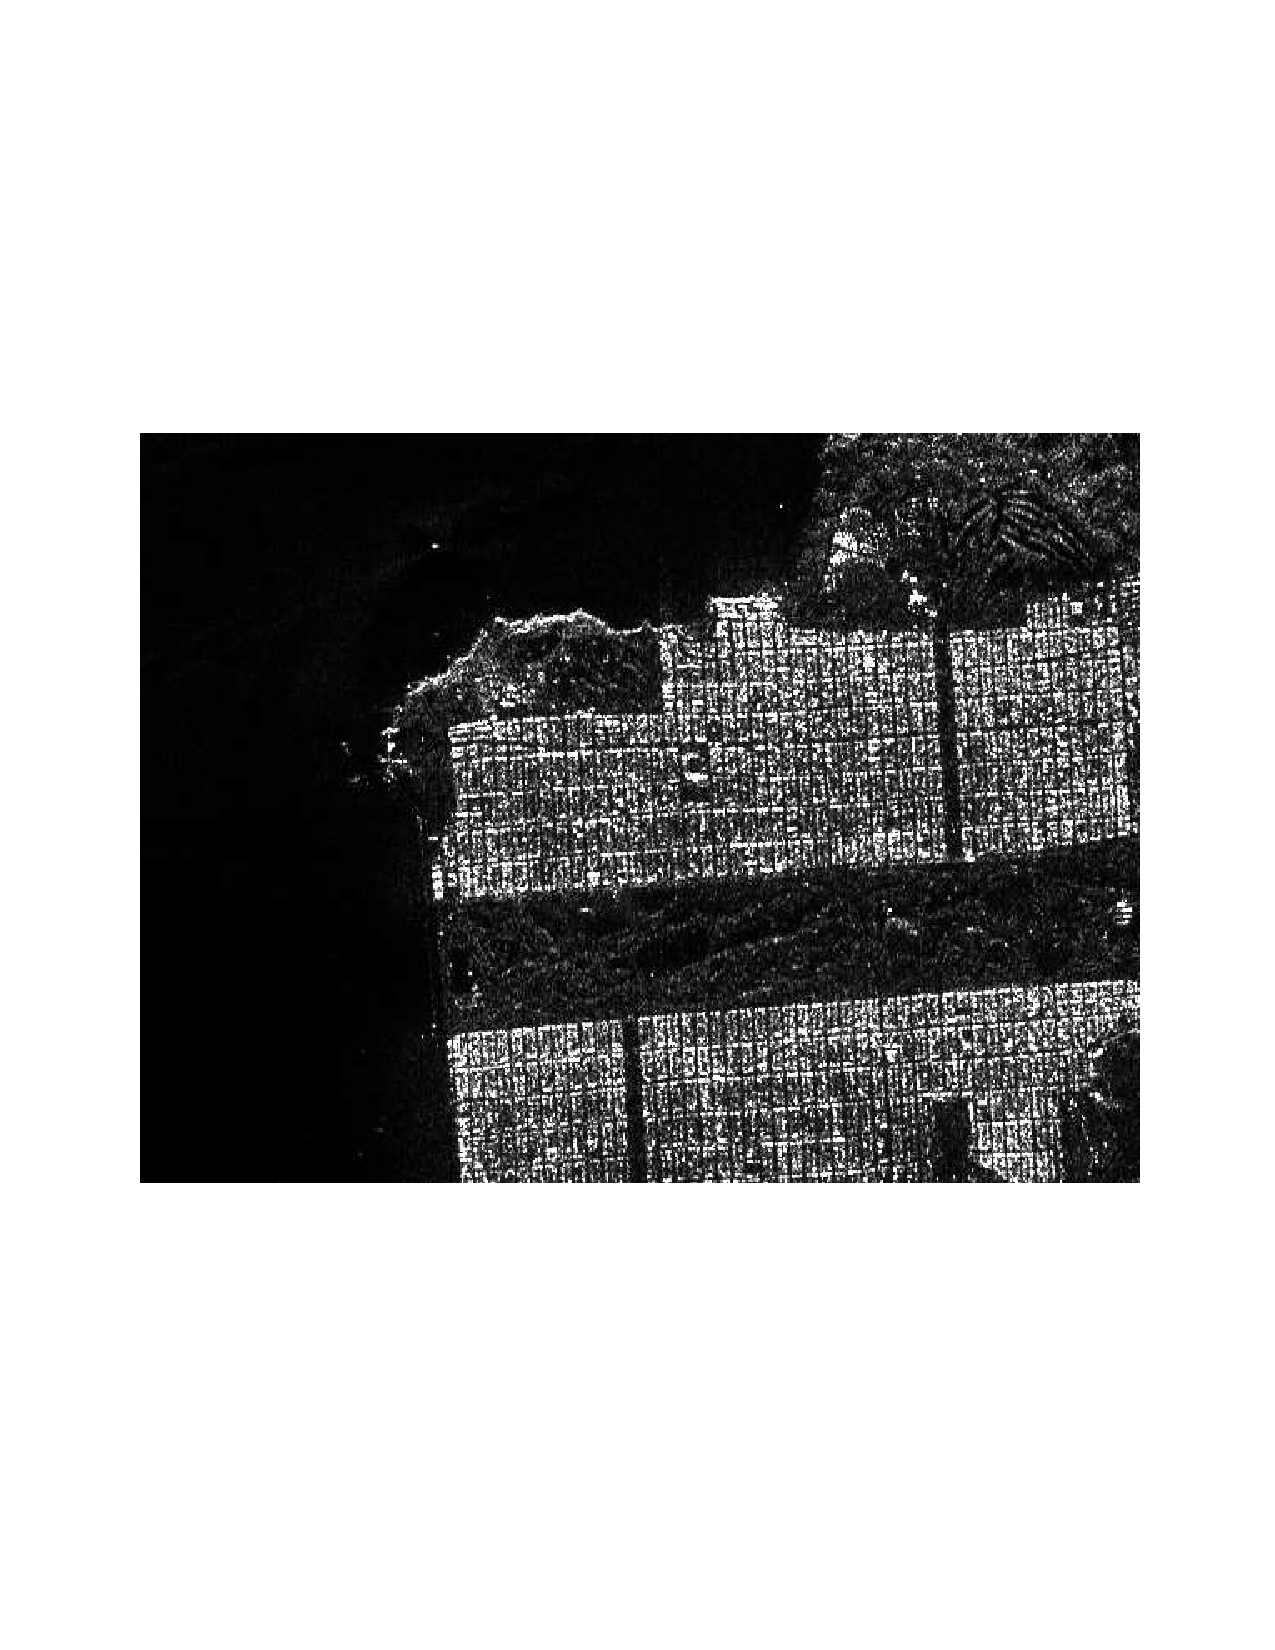
\includegraphics[width=\linewidth]{sf_hh.pdf}
\endminipage
\minipage{0.35\textwidth}
	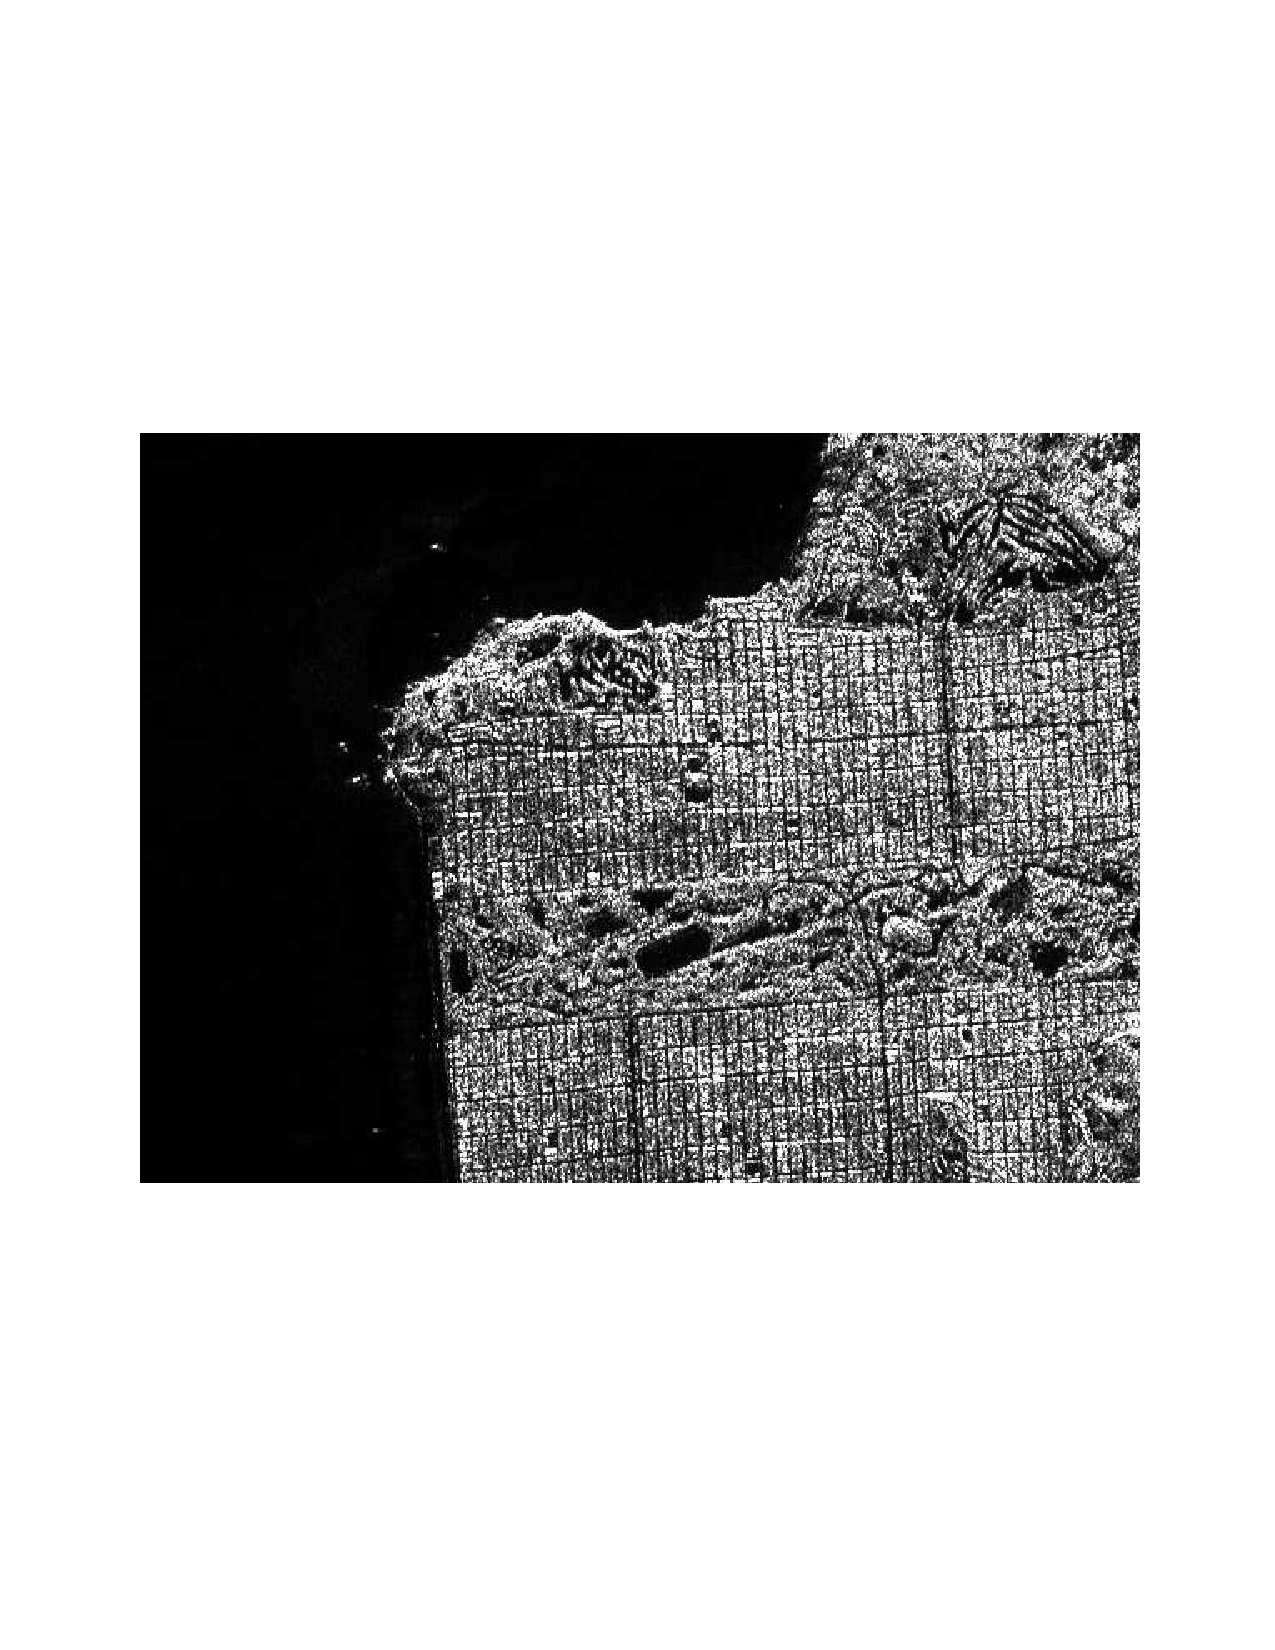
\includegraphics[width=\linewidth]{sf_vh.pdf}
\endminipage
\centering
\minipage{0.35\textwidth}
	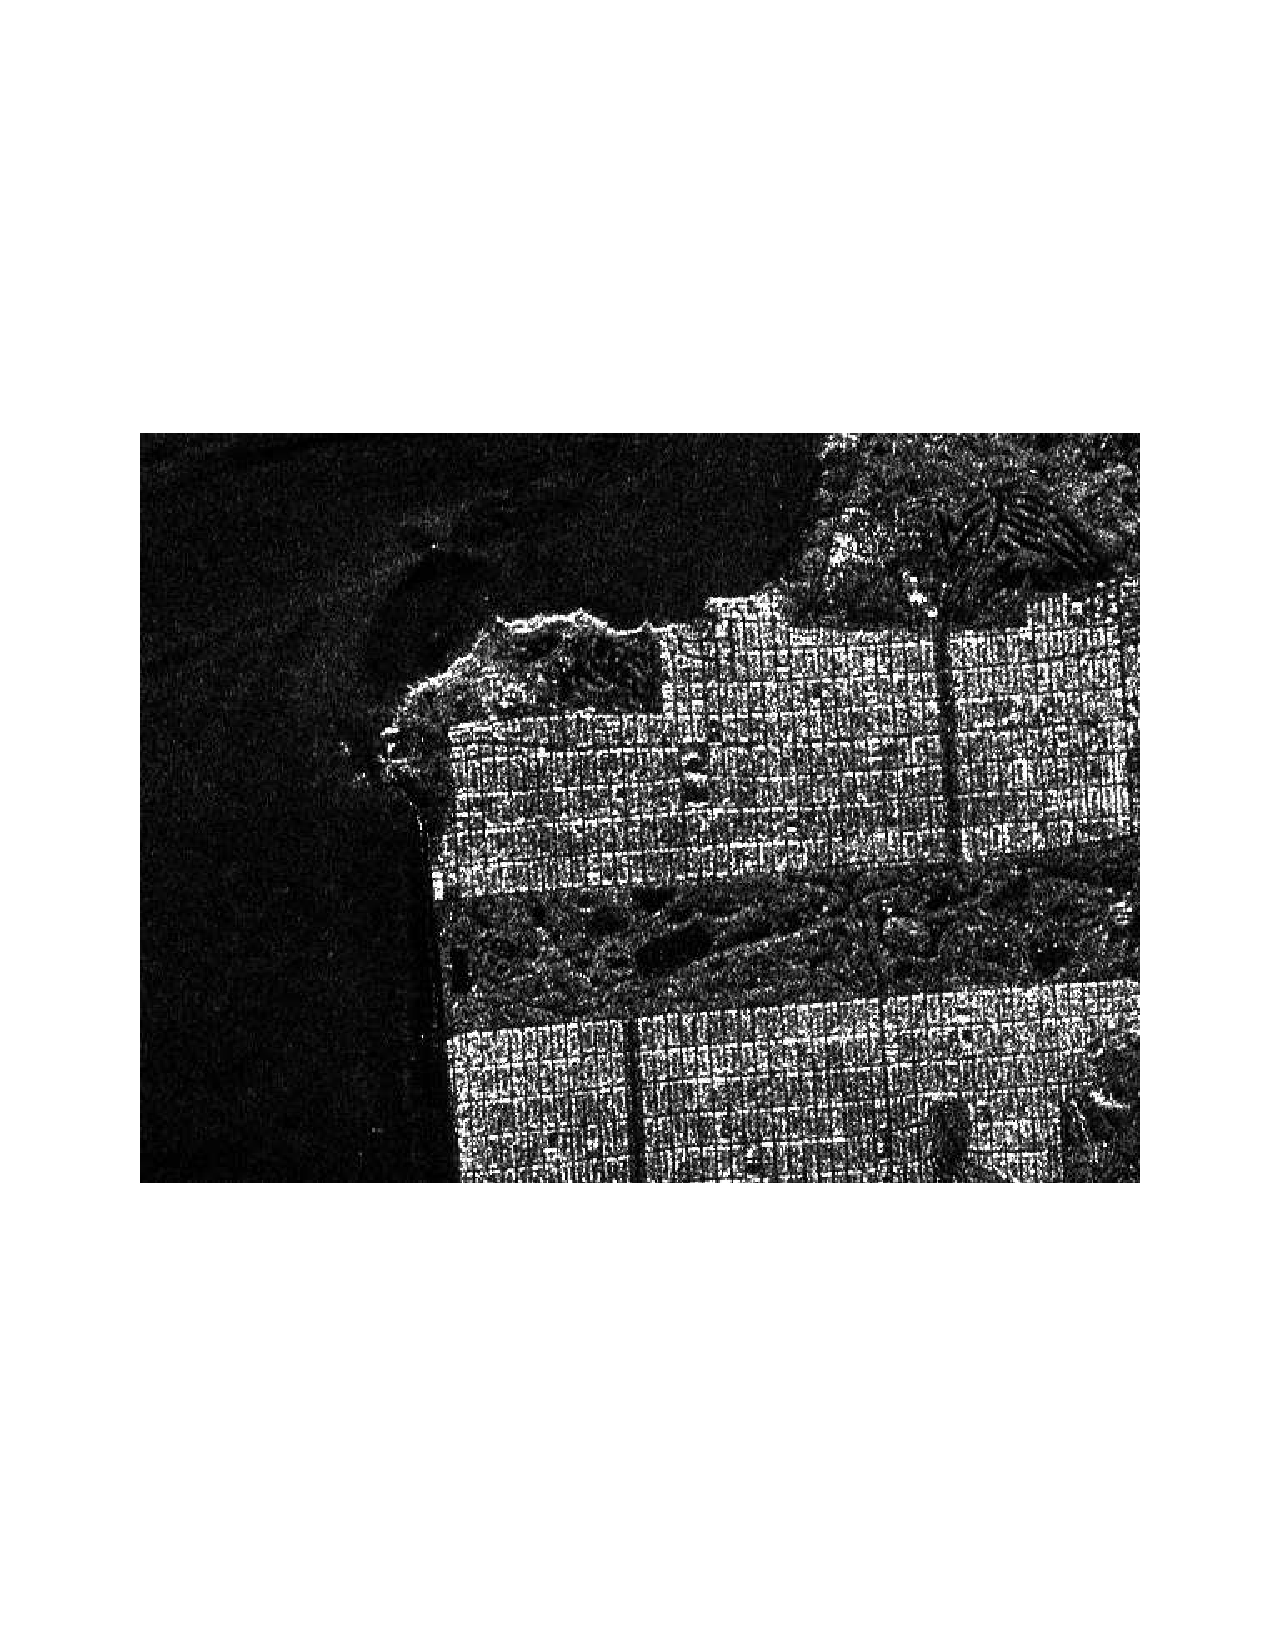
\includegraphics[width=\linewidth]{sf_vv.pdf}
\endminipage
        \vspace{-2.0cm}
	\caption{Imagem PolSAR com polarizações $HH$, $HV$ e $VV$.}\label{cap_acf_sf_hh_hv_vv}
\end{figure}

A visualização usando a decomposição RBG é mostrado na figura (\ref{cap_acf_sf_pauli}), sendo a maneira clássica como é conhecida a imagem da baía de São Franscisco. As figuras (\ref{cap_acf_sf_hh_blue}), (\ref{cap_acf_sf_hv_green}) e (\ref{cap_acf_sf_vv_red}) são respectivamente a decomposição RBG para cada canal $HH$ (azul), $HV$ (verde) e $VV$ (vermelho) das imagens PolSAR. 

\begin{figure}[hbt]
\begin{minipage}[b]{0.450\linewidth}
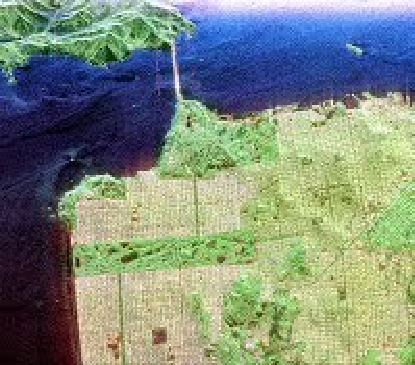
\includegraphics[width=\linewidth]{polsar_teste.pdf}
\caption{Baía de São Francisco.}
\label{cap_acf_sf_pauli}
\end{minipage}\hfill
\begin{minipage}[b]{0.450\linewidth}
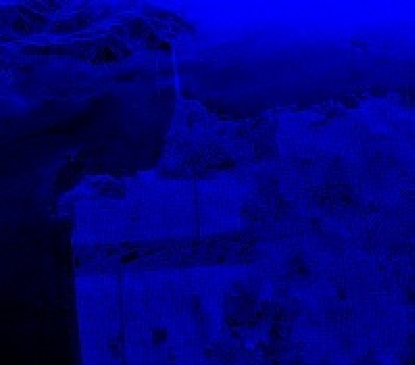
\includegraphics[width=\linewidth]{polsar_blue.pdf}
\caption{Polarização $HH$.}
\label{cap_acf_sf_hh_blue}
\end{minipage}
\end{figure}
%
\begin{figure}[hbt]
\begin{minipage}[b]{0.450\linewidth}
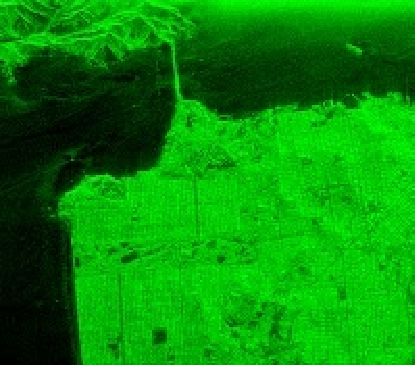
\includegraphics[width=\linewidth]{polsar_green.pdf}
\caption{Polarização $HV$.}
\label{cap_acf_sf_hv_green}
\end{minipage}\hfill
\begin{minipage}[b]{0.450\linewidth}
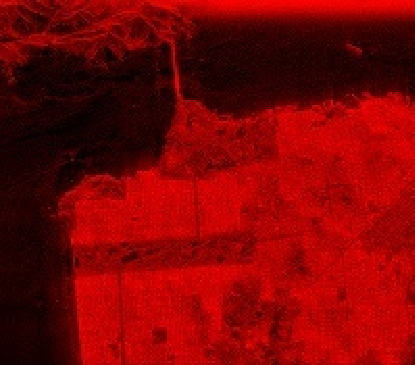
\includegraphics[width=\linewidth]{polsar_red.pdf}
\caption{Polarização $VV$.}
\label{cap_acf_sf_vv_red}
\end{minipage}
\end{figure}

Atualmente, podemos indicar tendências de aplicações de imagens SAR e PolSAR.  Existe interesse em desenvolver um sistema tipo SAR, com comprimentos de ondas óticos que podem ter uma resolução de $10\times 10$ centímetros quadrados, um exemplo é o  sistema Lynx projetado pelo laboratório nacional Sandia, o qual alcança resoluções de $10$ a $30$ centímetros quadrados. Existe ainda o mini-SAR para uso em veículos aéreos não tripulados que focam na evolução da micro-eletrônica para aumentar a eficiência e diminuir o peso. 

As imagens SAR podem ser captadas por satélites orbitando outros planetas como o projeto Magellan SAR orbitando Vênus.  Outra tecnologia usada para a captação  imagens SAR, chamada de interferométrica SAR (InSAR), que usa dois ou mais radares de abertura sintética para obter imagens.   
 
Os sistemas SAR e PolSAR apresentam algumas características inerentes do processo teórico e tecnológico que poderíamos destacar como desvantagens:
\begin{itemize}
\item requer o conhecimento da rota do radar;
\item o sistema SAR é sensível ao movimento do alvo;
\item o processamento para a geração de uma imagem é complexo.
\end{itemize}

Entretanto essas desvantagens nos sistemas SAR e PolSAR não evitam as mesmas de serem largamente empregadas, tornando a área do conhecimento muito ativa, gerando um grande interesse, tanto em nível de aplicação como em pesquisa científica.

\chapter{Metodologia}

\section{Modelagem estatística para dados PolSAR}\label{cap_acf_sec1}
Os sistemas SAR totalmente polarimétricos transmitem pulsos de micro-ondas polarizados ortogonalmente e medem componentes ortogonais do sinal recebido. Para cada pixel, a medida resulta em uma matriz de coeficientes de espalhamento. Esses coeficientes são números complexos que descrevem no sistema SAR a transformação do campo eletromagnético transmitido para o campo eletromagnético recebido.

A transformação pode ser representada como
\begin{equation}\label{cap_acf_1}
 \left[
\begin{array}{c}
	E_{h}^{r}   \\
	E_{v}^{r}    \\
\end{array}
\right]
 = \frac{e^{\hat{\imath} kr}}{r}\left[
\begin{array}{cc}
	S_{hh}   & S_{hv}   \\
	S_{vh}   & S_{vv}   \\
\end{array}
\right]
 \left[
\begin{array}{c}
	E_{h}^{t}   \\
	E_{v}^{t}    \\
\end{array}
\right],
\end{equation}
onde $k$ denota o número de onda, $\hat{\imath}$ é um número complexo e $r$ é a distância entre o radar e o alvo. O campo eletromagnético com componentes $E_{i}^{j}$, o índice subscrito denota polarização horizontal ($h$) ou vertical ($v$),  enquanto o índice sobrescrito indica a onda recebida ($r$) ou transmitida ($t$). Definindo $S_{i,j}$ como os coeficientes de espalhamento complexo, tal que o índice $i$ e $j$ são associados com o recebimento com a transmissão das ondas, por exemplo, o coeficiente de espalhamento $S_{hv}$ está associado a onda transmitida na direção vertical ($v$) e recebida na direção horizontal ($h$).

Sendo conhecido cada um dos coeficientes, a matriz de espalhamento complexa $\mathbf{S}$ é definida por
\begin{equation}\label{cap_acf_2}
\mathbf{S} = \left[
\begin{array}{cc}
	S_{hh}   & S_{hv}   \\
	S_{vh}   & S_{vv}   \\
\end{array}
\right],
\end{equation}
se o meio de propagação das ondas é recíproco, isto é, de uma maneira geral as propriedades de transmissão e recebimento de uma antena são idênticos, então usaremos o teorema da reciprocidade \citet{lp} para definir a matriz de espalhamento como sendo hermitiana, ou seja, a igualdade dos termos complexos $S_{hv}=S_{vh}$. De acordo com o teorema da reciprocidade a matriz de espalhamento pode ser representada pelo vetor
\begin{equation}\label{cap_acf_3}
\mathbf{s} = \left[
\begin{array}{c}
	S_{hh}      \\
        \sqrt{2}S_{vh}     \\
	S_{vv}      \\
\end{array}
\right].
\end{equation}

Podemos definir uma generalização para a representação de dados PolSAR com visada simples como sendo o vetor de espalhamento com polarização $m$, $$\mathbf{s}=[S_1,S_2,\dots,S_m]^H,$$ onde $H$ sobrescrito na representação vetorial significa o cáculo do número complexo conjugado e a seguida transposição do vetor. Os valores $S_j$ com $j=1,\dots,m$ representam variáveis randômicas complexas associadas com cada canal de polarização. De acordo com \citet{good} a distribuição gaussiana circular complexa multivariada com média zero pode modelar adequadamente o comportamento estatístico de $\mathbf{s}$.  

A função densidade de probabilidade ({\bf pdf}) da distribuição gaussiana complexa $m$-variada é dada por
\begin{equation}\label{cap_acf_4}
    p({\bf s})=\frac{1}{\pi^m|\bf{\Sigma}_{{\bf s}}|}\exp(-{\bf s}^{H}\bf{\Sigma}_{{\bf s}}^{-1}{\bf s}), 
\end{equation}
sendo $|\cdot|$ o determinante de uma matriz ou o valor absoluto de um escalar, e $\mathbf{\Sigma}_{\bf{s}}$ é a matriz de covariância associada a $\mathbf{s}$ definida por
\begin{equation}\label{cap_acf_5}
	{\bf \Sigma_{{\bf s}}} = E[{\mathbf s}{\mathbf s}^H] = \left[
\begin{array}{cccc}
	E[S_1\overline{S_1}]  & E[{S_1}\overline{S_2}] &\hdots & E[S_1\overline{S_m}] \\
	E[S_2\overline{S_1}]  & E[{S_2}\overline{S_2}] &\hdots &E[S_2\overline{S_m}]\\
        \vdots&\vdots &\ddots &\vdots\\
	E[S_m\overline{S_1}]  & E[S_m\overline{S_2}] &\hdots &E[S_m\overline{S_m}]\\
\end{array}
\right]
\end{equation}
talque, $E[\cdot]$ denota o valor esperado e $\overline{\cdot}$ denota o conjugado complexo. A matriz de covariância é hermitiana positiva definida e contém todas as informações necessárias para caracterizar o retroespalhamento, podemos consultar mais informações em \citep{mfp}. 

Nas imagens PolSAR serão consideradas três componentes para o vetor $\mathbf{s}=[S_{hh},S_{vh},S_{vv}]^T$ e a multiplicação de $\mathbf{s}=[S_{hh},S_{vh},S_{vv}]$ pelo seu conjugado transposto $\mathbf{s}=[S_{hh},S_{vh},S_{vv}]^H$, isto é, a hermitiana do vetor, 

\begin{equation}\label{cap_acf_6}
\mathbf{s}\mathbf{s}^H = \left[
\begin{array}{c}
	S_{hh}      \\
        S_{vh}     \\
	S_{vv}      \\
\end{array}
\right]
\left[
\begin{array}{ccc}
	S_{hh}  & S_{vh}  & S_{vv}      \\
\end{array}
\right]^H = 
\left[
\begin{array}{ccc}
	S_{hh}\overline{S_{hh}} & S_{hh} \overline{S_{vh}} & S_{hh}  \overline{S_{vv}}     \\
	S_{vh} \overline{S_{hh}}  & S_{vh} \overline{S_{vh}}  & S_{vh} \overline{S_{vv}}      \\
	S_{vv} \overline{S_{hh}}  & S_{vv} \overline{S_{vh}}  & S_{vv}  \overline{S_{vv}}     \\
\end{array}
\right].
\end{equation}

A  matriz $\mathbf \Sigma_{{\mathbf s}}$ tem dimensão $3\times 3$, e pode ser definida como sendo a matriz de covariância associada a $\mathbf{s}$.
\begin{equation}\label{cap_acf_7}
\mathbf{\Sigma_{{\mathbf s}}} = E[\mathbf{s}\mathbf{s}^H] =
\left[
\begin{array}{ccc}
	E[S_{hh}\overline{S_{hh}}] & E[S_{hh} \overline{S_{vh}}] & E[S_{hh}  \overline{S_{vv}}]     \\
	E[S_{vh} \overline{S_{hh}}]  & E[S_{vh} \overline{S_{vh}}]  & E[S_{vh} \overline{S_{vv}}]      \\
	E[S_{vv} \overline{S_{hh}}]  & E[S_{vv} \overline{S_{vh}}]  & E[S_{vv}  \overline{S_{vv}}]     \\
\end{array}
\right].  
\end{equation}

Dados polarimétricos são usualmente sujeitados a um processo de várias visadas com o intuito de melhorar a razão entre o sinal e o seu ruído. Para esse fim, matrizes positivas definidas hermitianas estimadas são obtidas computando a média de $L$ visadas independentes de uma mesma cena. Resultando na matriz de covariância amostral estimada {\bf Z} conforme \citep{good, ade}
\begin{equation}\label{cap_acf_8}
\begin{array}{ccc}
    \mathbf{Z}&=&\frac{1}{L}\displaystyle{\sum_{i=1}^{L} {\mathbf{s}_i}{\mathbf{s}_i}^H}, \\
\end{array}
\end{equation}
onde $\mathbf{s}_i$ com $i = 1, \dots, L$ é uma amostra de $\mathit{L}$ vetores complexos distribuídos como $\mathbf{s}$, assim a matriz de covariância amostral associada a $\mathbf{s}_i$, com $i=1,\dots,L$ denotam o espalhamento para cada visada $L$ seguindo uma distribuição complexas de Wishart. 

Sendo agora $\mathbf{\Sigma_{s}}$ e $L$ parâmetros conhecidos a função densidade de probabilidade da distribuição Wishart por  
%
\begin{equation}\label{cap_acf_9}
    f_{\mathbf{Z}}(\mathbf{Z};\mathbf{\Sigma_{s}},L)=\frac{L^{mL}|\mathbf{Z}|^{L-m}}{|\mathbf{\Sigma_{s}}|^{L}\Gamma_m(L)} \exp(-L\traco(\mathbf{\Sigma_{s}}^{-1}\mathbf{Z})), \\
\end{equation}
onde, $\traco(\cdot)$ é o operador traço de uma matriz, $\Gamma_m(L)$ é uma função Gamma multivariada definida por
\begin{equation}\label{cap_acf_10}
	\Gamma_m(L)=\pi^{\frac{1}{2}m(m-1)} \prod_{i=0}^{m-1}\Gamma(L-i) \\
\end{equation}
e $\Gamma(\cdot)$ é a função Gamma. Podemos afirmar que $\mathbf{Z}$ é distribuído como uma distribuição Wishart denotando por $\mathbf{Z}\sim W(\mathbf{\Sigma_{s}}, L)$ e satisfazendo $E[\mathbf{Z}]=\mathbf{\Sigma_{s}}$. Sem perda de generalidade para o texto vamos usar o simbolo $\mathbf{\Sigma}$ em detrimento a $\mathbf{\Sigma_{s}}$ para representar a matriz de covariância associada a $\mathbf{s}$.

Seja a função densidade de probabilidade da distribuição complexa Wishart (\ref{cap_acf_9}) na qual vamos aplicar o logaritmo natural e suas propriedades com o intuito de reescrever a função na forma adequada para aplicar o método de estimativa de máxima verossimilhança. Assim,
\begin{equation}\label{cap_acf_11}
\begin{array}{ccc}
    \ln{f_{\mathbf{Z}}(\mathbf{Z};\mathbf{\Sigma},L)}&=&\ln{\left(\frac{L^{mL}|\mathbf{Z}|^{L-m}}{|\mathbf{\Sigma}|^{L}\Gamma_m(L)} \exp(-L\traco(\mathbf{\Sigma}^{-1}\mathbf{Z}))\right)}, \\
        \ln{\left(f_{\mathbf{Z}}(\mathbf{Z};\mathbf{\Sigma},L)\right)}&=&\ln{\left(\frac{L^{mL}|\mathbf{Z}|^{L-m}}{|\mathbf{\Sigma}|^{L}\Gamma_m(L)}\right)}+\ln{\left( \exp(-L\traco(\mathbf{\Sigma}^{-1}\mathbf{Z}))\right)}, \\
        \ln{\left(f_{\mathbf{Z}}(\mathbf{Z};\mathbf{\Sigma},L)\right)}&=&\ln{\left(L^{mL}|\mathbf{Z}|^{L-m}\right)} - \ln{\left(|\mathbf{\Sigma}|^{L}\Gamma_m(L)\right)}-L\traco(\mathbf{\Sigma}^{-1}\mathbf{Z}), \\
        \ln{\left(f_{\mathbf{Z}}(\mathbf{Z};\mathbf{\Sigma},L)\right)}&=&mL\ln{L}+(L-m)\ln{\left(|\mathbf{Z}|\right)} - \ln{\left(|\mathbf{\Sigma}|^{L}\right)}-\ln{\left(\Gamma_m(L)\right)}-L\traco(\mathbf{\Sigma}^{-1}\mathbf {Z}), \\
	\ln{\left(f_{\mathbf{Z}}(\mathbf{Z};\mathbf{\Sigma},L)\right)}&=&mL\ln{L}+L\ln{\left(|\mathbf{Z}|\right)}-m\ln{\left(|\mathbf{Z}|\right)} - L\ln{\left(|\mathbf{\Sigma}|\right)}-\ln{\left(\Gamma_m(L)\right)}-L\traco(\mathbf{\Sigma}^{-1}\mathbf{Z}), \\
\end{array}
\end{equation}
lembrando que a função Gamma multivariada é definida na equação (\ref{cap_acf_10}) então, podemos rescrever a equação da seguinte forma
\begin{equation}\label{cap_acf_12}
\begin{array}{cll}
	\ln{\left(f_{\mathbf{Z}}(\mathbf{Z};\mathbf{\Sigma},L)\right)}&=&mL\ln{L}+L\ln{\left(|\mathbf{Z}|\right)}-m\ln{\left(|\mathbf{Z}|\right)} - L\ln{\left(|\mathbf{\Sigma}|\right)}-\ln{\left(\Gamma_m(L)\right)}-L\traco(\mathbf{\Sigma}^{-1}\mathbf{Z}), \\
	\ln{\left(f_{\mathbf{Z}}(\mathbf{Z};\mathbf{\Sigma},L)\right)}&=&mL\ln{L}+L\ln{\left(|\mathbf{Z}|\right)}-m\ln{\left(|\mathbf{Z}|\right)} - L\ln{\left(|\mathbf{\Sigma}|\right)}\\
	&-&\ln{\left(\pi^{\frac{1}{2}m(m-1)} \prod_{i=0}^{m-1}\Gamma(L-i)\right)}-L\traco(\mathbf{\Sigma}^{-1}\mathbf{Z}),\\
	\ln{\left(f_{\mathbf{Z}}(\mathbf{Z};\mathbf{\Sigma},L)\right)}&=&mL\ln{L}+L\ln{\left(|\mathbf{Z}|\right)}-m\ln{\left(|\mathbf{Z}|\right)} - L\ln{\left(|\mathbf{\Sigma}|\right)}\\
        &-&\ln{\left(\pi^{\frac{1}{2}m(m-1)}\right)}-\ln{\left( \prod_{i=0}^{m-1}\Gamma(L-i)\right)}-L\traco(\mathbf{\Sigma}^{-1}\mathbf{Z}), \\
	\ln{\left(f_{\mathbf{Z}}(\mathbf{Z};\mathbf{\Sigma},L)\right)}&=&mL\ln{L}+L\ln{\left(|\mathbf{Z}|\right)}-m\ln{\left(|\mathbf{Z}|\right)} - L\ln{\left(|\mathbf{\Sigma}|\right)}\\
        &-&\frac{1}{2}m(m-1)\ln{\left(\pi\right)}-\sum_{i=0}^{m-1}\ln{\left(\Gamma(L-i)\right)}-L\traco(\mathbf{\Sigma}^{-1}\mathbf{Z}),\\
\end{array}
\end{equation}
equação equivalente pode ser encontrada em \citep{fnc2011}.

\section{Detecção de bordas em imagens PolSAR}\label{cap_acf_sec2}

Na literatura encontramos uma grande oferta de métodos clássicos para detectar bordas, por exemplo Sobel, Canny, Laplaciano da gaussiana(LoG) e LoG piramidal. Os métodos clássicos de detecção de bordas são construídos assumindo que o ruído é aditivo, tornando esses métodos ineficientes para aplicação em imagens PolSAR, entretanto, nas imagens PolSAR o ruído é multiplicativo. 

Na corrente seção conceitos baseados nos artigos \citet{nhfc, gmbf} serão introduzidos e proporemos modificações para os métodos de detecção de borda em imagens PolSAR com multiplas visadas. A ideia principal é detectar o ponto de transição em uma faixa tão fina quanto possível entre duas regiões da imagem. O ponto de transição é definido como uma evidência de borda. Os ruídos nesse tipo de imagens são do tipo \textit{speckle}, os mesmos têm natureza multiplicativa, tornando a detecção de bordas em imagens SAR uma tarefa desafiadora.

Podemos indicar que o problema de detecção de bordas, pode ser resumido em três importantes aspectos:
\begin{enumerate}
	\item o procedimento para detecção;
	\item a determinação de uma posição mais acurada da posição da borda;
	\item a especificação de tamanho para uma janela (pode ser uma janela quadrada ou em uma faixa de dados). 
\end{enumerate}

O tamanho da janela pode influenciar em alguns aspectos como por exemplo, em uma janela pequena pode não conter informações para identificar a presença de bordas, ou em janelas maiores podem obter informações para mais de uma borda. Assim o tamanho de janela ideal é aquele que contém as informações para detecção de uma borda. Vamos assumir que há uma borda na janela fornecida pela seleção inicial, quando forem realizados os testes computacionais.

Em linhas gerais seguiremos as seguintes afirmações: 
\begin{enumerate}
	\item tentar encontrar finas faixas de dados, idealmente do tamanho de um pixel;
	\item será usado o método de máxima verossimilhança;
	\item de que maneira a detecção trabalha em diferentes canais da imagem PolSAR. 
\end{enumerate}

De uma maneira geral, a ideia se baseia em encontrar um ponto de transição em uma faixa de dados, o qual é considerado uma estimativa de posicionamento da borda, isto é, uma evidência de borda. A evidência de borda é encontrada em um processo de otimização. 

As metodologias de detecção de bordas ocorrem em diversos estágios, abaixo enumeramos os estágios:
\begin{enumerate}
	\item identificar o centroide de uma região de interesse (ROI) de maneira automática, semiautomática ou manual;
	\item construir raios do centroide para fora da área de interesse;
	\item coletar dados em uma vizinhança em torno dos raios;
	\item detectar pontos na faixa de dados os quais fornecem evidências de mudanças de propriedades estatística, ou seja, uma transição que define uma evidência de borda;
	\item definir o contorno usando um método de interpolação entre os pontos de transição, por exemplo, as B-Splines, ou o método dos quadrados mínimos \textbf{MMQ}.
\end{enumerate}

Inicialmente, escolhemos uma região de interesse (ROI) $\mathbf{R}$ com centroide $\mathbf{C}$ e traçamos raios iniciando em $\mathbf{C}$ e indo até um ponto de controle $\mathbf{P}_i$, com $i=1,2,\dots, \mathbf{S}$, estes pontos de controle estão fora da região $\mathbf{R}$. Teremos $\mathbf{S}$ raios resultantes representados por ${\bf s^{(i)}}=\overline{\mathbf{CP}_i}$ com ângulos $\epsilon_{i}=\angle ({\bf s_{(i)}},{\bf s_{(i+1)}})$. 

Os raios serão convertidos sobre pixeis usando o algoritmo {\it Bresenham's midpoint line algorithm}, esse algoritmo fornece uma fina representação digital para os raios. Portanto, em cada raio vamos assumir que os dados seguem uma distribuição complexa Wishart com sua respectiva função de distribuição dada por (\ref{cap_acf_9}) e denotada por $W(\Sigma,L)$.

A faixa de dados coletada no $\mathit{i}$ - ésimo raio $\mathbf{s^{i}}$, com $i$ variando em $i=1,2,\dots, S$, contém $N^{(i)}$ pixeis. Para cada pixel $\mathit{k}$ em uma dada faixa $\mathit{i}$, a mesma pode ser descrita pelo resultado da matriz $Z_{k}^{(i)}$ sendo esta uma distribuição de Wishart, portanto podemos representar cada pixel como uma distribuição,  
\begin{equation}\label{cap_acf_13}
 \left\{
\begin{array}{cl}
	Z_{k}^{(i)}\sim W(\Sigma_{A}^{(i)},L_{A}^{(i)}),& \mbox{para}\quad k=1,\dots,j^{(i)} , \\
	Z_{k}^{(i)}\sim W(\Sigma_{B}^{(i)},L_{B}^{(i)}),& \mbox{para}\quad k=j^{(i)} + 1,\dots,N^{(i)}.  \\
\end{array}
\right.
\end{equation}

Podemos definir cada faixa composta de dois tipos de amostras, e, cada tipo obedece uma lei de Wishart complexa com diferentes parâmetros. Vamos assumir que o número de visadas é constante para todas as faixas. A ideia principal é encontrar uma evidência de borda $j^{(i)}$ em cada faixa, ao longo do raio ${\bf s^{(i)}}$, a evidência de borda ou ponto de transição representa um pixel de transição entre as duas amostras. O modelo proposto em (\ref{cap_acf_13}) assume que existir uma transição ocorrendo ao longo da faixa $\bf s^{(i)}$. Sem perda de generalidade na continuidade do trabalho será omitido o índice $(i)$ focando nossa análise em uma única faixa.
% *******************************************************
\section{Estimativa por Máxima verossimilhança (\textbf{MLE})}\label{cap_acf_sec3}

O conceito de verossimilhança é importante em estatística, pois descreve de maneira precisa as informações sobre os parâmetros do modelo estatístico que representa os dados observados. De maneira geral, a estimativa por máxima verossimilhança (\textbf{MLE}) é um método que, tendo um conjunto de dados e um modelo estatístico, estima os valores dos parâmetros do modelo estatísticos com intuito de maximizar uma função de probabilidade dos dados. 

\section{Função de verossimilhança}

Suponha $\mathbf{X}=(X_1,X_2,\dots,X_n)^T$ um vetor randômico distribuído de acordo com a $\mathbf{p.d.f}$ função densidade de probabilidade $f(\mathbf{x},\mathbf{\theta})$ com parâmetros $\mathbf{\theta}=(\theta_1,\dots,\theta_d)^T$ no espaço dos parâmetros $\Theta$. Definimos  a \textbf{função de verossimilhança} cuja amostra é 
\begin{equation}\label{cap_acf_14}
    L(\theta;\mathbf{X}) = \prod_{i=1}^{n}f(x_i;\theta), \\
\end{equation}
e a função logarítmica de verossimilhança a qual podemos chamar de  \textbf{função de log-verossimilhança} é a soma
\begin{equation}\label{cap_acf_15}
	l(\theta;\mathbf{X})= \ln(L(\theta;\mathbf{X})) = \sum_{i=1}^{n}\ln(f(x_i;\theta)). \\
\end{equation}

Podemos definir o método da \textbf{estimativa de máxima verossimilhança} (\textbf{MLE}) de $\theta$ como sendo o vetor $\widehat{\theta}$ tal que $L(\widehat{\theta};\mathbf{x})\ge L(\theta;\mathbf{x})$ para todo $\theta$ no espaço dos parâmetros $\Theta$. De maneira simplificada a \textbf{estimativa de máxima verossimilhança} pode ser escrita por 
\begin{equation}\label{cap_acf_16}
    \widehat{\theta}= \text{arg}\,\max\limits_{\theta\in\Theta}L(\theta;\mathbf{x}),\\
\end{equation}
ou de maneira similar 
\begin{equation}\label{cap_acf_17}
    \widehat{\theta}= \text{arg}\,\max\limits_{\theta\in\Theta}l(\theta;\mathbf{x}).\\
\end{equation}

\section{Estimativa de máxima verossimilhança aplicada a distribuíção Wishart}

Nesta seção vamos usar o método de máxima verossimilhança aplicado na distribuição Wishart. Suponha $\mathbf{Z}=(\mathbf{Z}_1,\mathbf{Z}_2,\dots,\mathbf{Z}_N)^T$ um vetor randômico distribuído de acordo com a $\mathbf{p.d.f}$ função densidade de probabilidade (\ref{cap_acf_9}) com parâmetros $\Sigma=\{\mathbf{\Sigma_A}, \mathbf{\Sigma_B\}}$ e $L$.

A \textbf{função de verossimilhança} da amostra descrita por (\ref{cap_acf_13}) é dada pela equação produtório das funções de densidade respectivamente associadas a cada amostra
\begin{equation}\label{cap_acf_18}
	L(j)=\prod_{k=1}^{j}f_{\mathbf{Z}}(\mathbf{Z}_{k}^{'};\mathbf{\Sigma_{A}},L) \prod_{k=j+1}^{N}f_{\mathbf{Z}}(\mathbf{Z}_{k}^{'};\mathbf{\Sigma_{B}},L), \\
\end{equation}
onde $\mathbf{Z}_{k}^{'}$ é uma possível aproximação da matriz randômica descrita em (\ref{cap_acf_13}).

Usando a equação (\ref{cap_acf_12}) e propriedades de logaritmos natural teremos para cada termo do produtório (\ref{cap_acf_18}) uma \textbf{função de log-verossimilhança}. Assim, encontramos uma função dependente de $j$
\begin{equation}\label{cap_acf_19}
	l(j)=\ln L(j)=\sum_{k=1}^{j}\ln f_{\mathbf{Z}}(\mathbf{Z}_{k}^{'};\mathbf{\Sigma_{A}},L)+ \sum_{k=j+1}^{N}\ln f_{\mathbf{Z}}(\mathbf{Z}_{k}^{'};\mathbf{\Sigma_{B}},L).
\end{equation}

Nesse momento, podemos realizar  manipulações algébricas na função distribuição em cada termo do somatório conforme (\ref{cap_acf_12}) e substituir nas duas parcelas da equação (\ref{cap_acf_19}) levando em consideração que as duas amostras são diferentes, desta forma
\begin{equation*}
\begin{array}{rcl}
	l(j)&=&\sum_{k=1}^{j}\left[mL\ln{\left(L\right)}+(L-m)\ln{\left(|\mathbf{Z}_{k}^{'}|\right)}- L\ln{\left(|\mathbf{\Sigma_{A}}|\right)}-\ln{\left(\Gamma_m(L)\right)}-L tr(\mathbf{\Sigma_{A}}^{-1}\mathbf{Z}_{k}^{'}))\right], \\
	&+&\sum_{k=j+1}^{N}\left[mL\ln{\left(L\right)}+(L-m)\ln{\left(|\mathbf{Z}_{k}^{'}|\right)}- L\ln{\left(|\mathbf{\Sigma_{B}}|\right)}-\ln{\left(\Gamma_m(L)\right)}-L tr(\mathbf{\Sigma_{B}}^{-1}\mathbf{Z}_{k}^{'})\right], \\
	l(j)&=&\sum_{k=1}^{N}\left[mL\ln{\left(L\right)}-\ln{\left(\Gamma_m(L)\right)}\right]-\sum_{k=1}^{j}\left[ L\ln{\left(|\mathbf{\Sigma_{A}}|\right)}-L tr(\mathbf{\Sigma_{A}}^{-1}\mathbf{Z}_{k}^{'}))\right], \\
	&+&\sum_{k=1}^{N}\left[(L-m)\ln{\left(|\mathbf{Z}_{k}^{'}|\right)}\right]- \sum_{k=j+1}^{N}\left[L\ln{\left(|\mathbf{\Sigma_{B}}|\right)}-L tr(\mathbf{\Sigma_{B}}^{-1}\mathbf{Z}_{k}^{'})\right], \\
	l(j)&=&N\left[mL\ln{\left(L\right)}-\ln{\left(\Gamma_m(L)\right)}\right]-L\left[j\ln{\left(|\mathbf{\Sigma_{A}}|\right)} +\sum_{k=1}^{j}tr(\mathbf{\Sigma_{A}}^{-1}\mathbf{Z}_{k}^{'})\right], \\
	&+&(L-m)\sum_{k=1}^{N}\ln{\left(|\mathbf{Z}_{k}^{'}|\right)}-L\left[(N-j)\ln{\left(|\mathbf{\Sigma_{B}}|\right)}+ \sum_{k=j+1}^{N}tr(\mathbf{\Sigma_{B}}^{-1}\mathbf{Z}_{k}^{'})\right], \\
	l(j)&=&N\left[mL\ln{\left(L\right)}-\ln{\left(\Gamma_m(L)\right)}\right]-L\left[j\ln{\left(|\mathbf{\Sigma_{A}}|\right)} +(N-j)\ln{\left(|\mathbf{\Sigma_{B}}|\right)}\right], \\
	&+&(L-m)\sum_{k=1}^{N}\ln{\left(|\mathbf{Z}_{k}^{'}|\right)}-L\left[\sum_{k=1}^{j}tr(\mathbf{\Sigma_{A}}^{-1}\mathbf{Z}_{k}^{'})+ \sum_{k=j+1}^{N}tr(\mathbf{\Sigma_{B}}^{-1}\mathbf{Z}_{k}^{'})\right]. \\
\end{array}
\end{equation*}

A matriz $\Sigma$ pode ser encontrada usando o estimador de máxima verossimilhança denotado por $\widehat{\Sigma}$ de acordo com a referência \citep{good}. A equação (\ref{cap_acf_20}) representa duas estimativa para a matriz de covariância $\Sigma$ que dependem da posição $j$
\begin{equation}\label{cap_acf_20}
\widehat{\Sigma_{I}}(j) = \left\{
\begin{array}{lc}
	j^{-1}\sum_{k=1}^{j}\mathbf{Z}_{k}  & \mbox{se}\quad I=A,  \\
        (N-j)^{-1}\sum_{k=j+1}^{N}\mathbf{Z}_{k} & \mbox{se}\quad I=B. \\
\end{array}
\right.
\end{equation}

Usando a equação (\ref{cap_acf_20}) podemos substituir na equação acima e continuar a manipulação algébrica
\begin{equation*}
\begin{array}{rcl}
	l(j)&=&N\left[mL\ln{\left(L\right)}-\ln{\left(\Gamma_m(L)\right)}\right]-L\left[j\ln{\left(|\mathbf{\Sigma_{A}}|\right)} +(N-j)\ln{\left(|\mathbf{\Sigma_{B}}|\right)}\right], \\
	&+&(L-m)\sum_{k=1}^{N}\ln{\left(|\mathbf{Z}_{k}^{'}|\right)}-L\left[\sum_{k=1}^{j}tr(\mathbf{\Sigma_{A}}^{-1}\mathbf{Z}_{k}^{'})+ \sum_{k=j+1}^{N}tr(\mathbf{\Sigma_{B}}^{-1}\mathbf{Z}_{k}^{'})\right], \\
	l(j)&=&N\left[mL\ln{\left(L\right)}-\ln{\left(\Gamma_m(L)\right)}\right]-L\left[j\ln{\left(|\mathbf{\Sigma_{A}}|\right)} +(N-j)\ln{\left(|\mathbf{\Sigma_{B}}|\right)}\right], \\
	&+&(L-m)\sum_{k=1}^{N}\ln{\left(|\mathbf{Z}_{k}^{'}|\right)}-L\left[tr\left(\sum_{k=1}^{j}\mathbf{\Sigma_{A}}^{-1}\mathbf{Z}_{k}^{'}\right)+tr\left( \sum_{k=j+1}^{N}\mathbf{\Sigma_{B}}^{-1}\mathbf{Z}_{k}^{'}\right)\right], \\
	l(j)&=&N\left[mL\ln{\left(L\right)}-\ln{\left(\Gamma_m(L)\right)}\right]-L\left[j\ln{\left(|\mathbf{\Sigma_{A}}|\right)} +(N-j)\ln{\left(|\mathbf{\Sigma_{B}}|\right)}\right], \\
	&+&(L-m)\sum_{k=1}^{N}\ln{\left(|\mathbf{Z}_{k}^{'}|\right)}-L\left[tr\left(\mathbf{\Sigma_{A}}^{-1}\sum_{k=1}^{j}\mathbf{Z}_{k}^{'}\right)+tr\left( \mathbf{\Sigma_{B}}^{-1}\sum_{k=j+1}^{N}\mathbf{Z}_{k}^{'}\right)\right], \\
	l(j)&=&N\left[mL\ln{\left(L\right)}-\ln{\left(\Gamma_m(L)\right)}\right]-L\left[j\ln{\left(|\mathbf{\Sigma_{A}}|\right)} +(N-j)\ln{\left(|\mathbf{\Sigma_{B}}|\right)}\right], \\
	&+&(L-m)\sum_{k=1}^{N}\ln{\left(|\mathbf{Z}_{k}^{'}|\right)}-L\left[mj+(N-j)m\right], \\
	l(j)&=&N\left[mL\ln{\left(L\right)}-\ln{\left(\Gamma_m(L)\right)}\right]-L\left[j\ln{\left(|\mathbf{\Sigma_{A}}|\right)} +(N-j)\ln{\left(|\mathbf{\Sigma_{B}}|\right)}\right], \\
	&+&(L-m)\sum_{k=1}^{N}\ln{\left(|\mathbf{Z}_{k}^{'}|\right)}-LNm, \\
	l(j)&=&N\left[-mL(1-\ln{\left(L\right)})-\ln{\left(\Gamma_m(L)\right)}\right]-L\left[j\ln{\left(|\mathbf{\Sigma_{A}}|\right)} +(N-j)\ln{\left(|\mathbf{\Sigma_{B}}|\right)}\right], \\
	&+&(L-m)\sum_{k=1}^{N}\ln{\left(|\mathbf{Z}_{k}^{'}|\right)}, \\
\end{array}
\end{equation*}
portanto, 
\begin{equation}\label{cap_acf_21}
\begin{array}{rcl}
	l(j)&=&N\left[-mL(1-\ln{\left(L\right)})-\ln{\left(\Gamma_m(L)\right)}\right]-L\left[j\ln{\left(|\mathbf{\widehat{\Sigma}}_{A}(j)|\right)} +(N-j)\ln{\left(|\mathbf{\widehat{\Sigma}}_{B}(j)|\right)}\right], \\
	&+&(L-m)\sum_{k=1}^{N}\ln{\left(|\mathbf{Z}_{k}^{'}|\right)}. \\
\end{array}
\end{equation}

O estimador de máxima verossimilhança $\widehat{\jmath}_{ML}$ é uma evidência de borda por representar uma aproximação da transição de região e pode ser calculado pelo método de maximização
\begin{equation}\label{cap_acf_22}
\begin{array}{rcl}
	\widehat{\jmath}_{ML}&=&\text{arg}\max\limits_{j}l(j).  \\
\end{array}
\end{equation}
% ****************************************************************
\chapter{Experimentos numéricos}
\section{Aplicação em imagens sintéticas}\label{cap_acf_sec4}

A metodologia (\textbf{MLE}) desenvolvida na seção anterior será aplicada em uma imagem sintética baseada no artigo \citep{gamf}, as quais são chamadas de \textit{Phantons}. As figuras desta seção serão geradas com auxílio dos códigos na linguagem Matlab, os programas foram disponibilizados pelos autores do artigo e estão localizados em  \url{http://www.ctim.es/polsar/}.

Inicialmente vamos gerar uma imagem sintética de dimensão $400\times400$ com duas amostras ou duas classes para validar as ideias do método (\textbf{MLE}), dessa maneira, vamos descrever como geramos a figura (\ref{cap_acf_fig01}). 

As imagens sintéticas em geral tem o intuito de auxiliar no estudo de diferentes métodos para tratamento de imagens. As imagens sintéticas construídas nesta seção  terão a tarefa de estudar como ocorre a transição entre duas amostras, ou seja, detectar evidências de bordas. 

A imagem PolSAR simulada usa a combinação de  matrizes de covariância $\{\Sigma_{k}\}_{k=1\dots 2}$ extraídas de uma imagem PolSAR real, com auxílio da distribuição complexa de Wishart $W_G(\Sigma, L)$, adicionalmente, na presente seção, os experimentos apresentados usam número de visadas $L=4$.

Para cada par de matrizes de covariância $\Sigma_{k_1}$, $\Sigma_{k_2}$ (com $k_2>k_1$) será gerado uma imagem PolSAR $P_{k_1,k_2,\beta}$ da seguinte maneira, em cada pixel branco da imagem sintética será agregado a amostra proveniente de $W_G(\Sigma_{k_1}, L)$ e de cada pixel preto da imagem sintética será agregado a amostra proveniente de $W_G(\Sigma_{k_2},L)$. Se necessário podemos fazer mistura de duas amostras tomando a combinação linear $W_G(\beta\Sigma_{k_1}+(1-\beta)\Sigma_{k_2}, L)$ com $\beta\in[0,1]$.

O parâmetro $\beta$ é usado para ponderar as informações entre as matrizes de covariância $\Sigma_{k_1}$ e $\Sigma_{k_2}$, modelando a mistura de classes em imagens PolSAR. Quando $\beta=0$ não há mistura e o problema consiste em escolher entre amostras puras de $\Sigma_{k_1}$ e $\Sigma_{k_2}$. Se o parâmetro $\beta$ se aproxima de $1$, teremos uma aproximação com a matriz de covariância $\Sigma_{k_1}$, assim teremos maior dificuldade de escolher classes. 

\begin{figure}[hbt]
\centering
	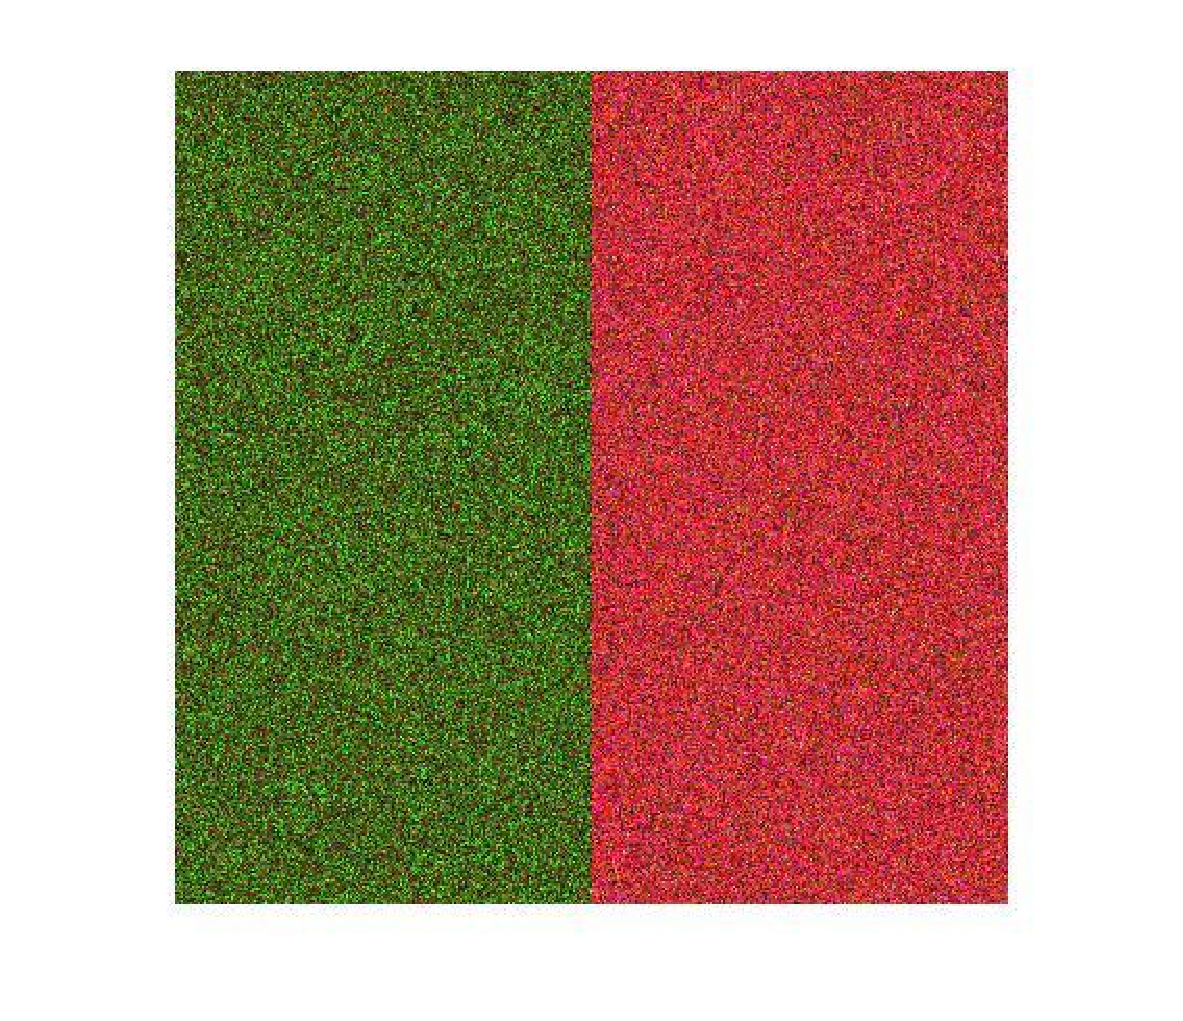
\includegraphics[width=5.0in]{phanton_nhfc_dec_pauli.pdf}
	\caption{Decomposição de Pauli para a phanton proposta no artigo de \citet{nhfc}.}\label{cap_acf_fig01}
\end{figure}
%%% ACF A decomposição de Pauli foi definida?
%%% AAB ver onde é melhor definir a decomposição de Pauli
A decomposição de Pauli foi usada na imagem mostrada na figura (\ref{cap_acf_fig01}), sendo que a mesma usa três canais da imagem \textbf{I} que são $\mathbf{I_{hh}}$, $\mathbf{I_{hv}}$ e $\mathbf{I_{vv}}$. 
	
\section{Aplicação do método \text{MLE} para duas classes definidas}

As informações sobre a imagem PolSAR podem ser obtidas de forma relativa pelos dados polarimétricos com respeito a um canal de dados, com intuito de resolver o problema de detecção bordas. Assumindo que o número de visadas $L$ e a matriz de covariância  $\Sigma$ são parâmetros na distribuição de Wishart, podemos descrever a distribuição gamma em cada canal, com densidade dada por 
\begin{equation}\label{cap_acf_23}
	f_{Z_{i}}(Z_{i};\frac{L}{\sigma_{i}^2},L)=\frac{L^{L}Z_{i}^{L-1}}{\sigma_{i}^{2L}\Gamma(L)} \exp(-L\frac{Z_{i}}{\sigma_{i}^2}), \\
\end{equation}
sendo $i\in \{HH, VH, VV\}$, $\sigma_{i}^2$ a entrada $(i,i)$ da matriz $\Sigma$ e $Z_{i}$ a entrada $(i,i)$ da matriz randômica $\mathbf{Z}$. Podemos verificar essa expressão em \citep{fnc, nhfc, hsbmp}.	 

O primeiro teste numérico será realizado com $\Sigma_u$ e $\Sigma_f$ definidas por
\begin{equation}\label{cap_acf_24}
	\hspace{2.75cm} \Sigma_{u}= \left[
\begin{array}{lll}
	962892             &19171 - 3579i&     -154638 + 191388i \\
	0.1917 + 0.0359i   &56707        &     -5798 + 16812i  \\
	-154638 - 191388i  &-5798 - 16812i&      472251 
\end{array}
\right],
\end{equation}
\begin{equation}\label{cap_acf_25}
 \Sigma_{f}= \left[
\begin{array}{lll}
	360932            & 11050 + 3759i&   63896 + 1581i \\
	0.1105 - 0.0376i  & 98960       &   6593 + 6868i \\
	63896  - 1581i    & 6593  - 6868i&   208843
\end{array}
\right],
\end{equation}
onde os subescritos $u$ e $f$ definem respectivamente área urbana e floresta, extraídas de uma imagem real, podemos encontrar essas informações nos artigos \citep{fbgm, nhfc}.

De acordo com a função densidade de probabilidade (\ref{cap_acf_23}) e usando o canal $(hh)$ em ambas matrizes de covariância com $L=4$, podemos gerar a figura (\ref{cap_acf_fig02}), com a representação gráfica da função de densidade para os respectivos elementos $u$ e $f$ da matriz de covariância, neste caso, $\sigma_{hh}=962892$ e $\sigma_{hh}= 360932$. 

\begin{figure}[hbt]
	\centering
	%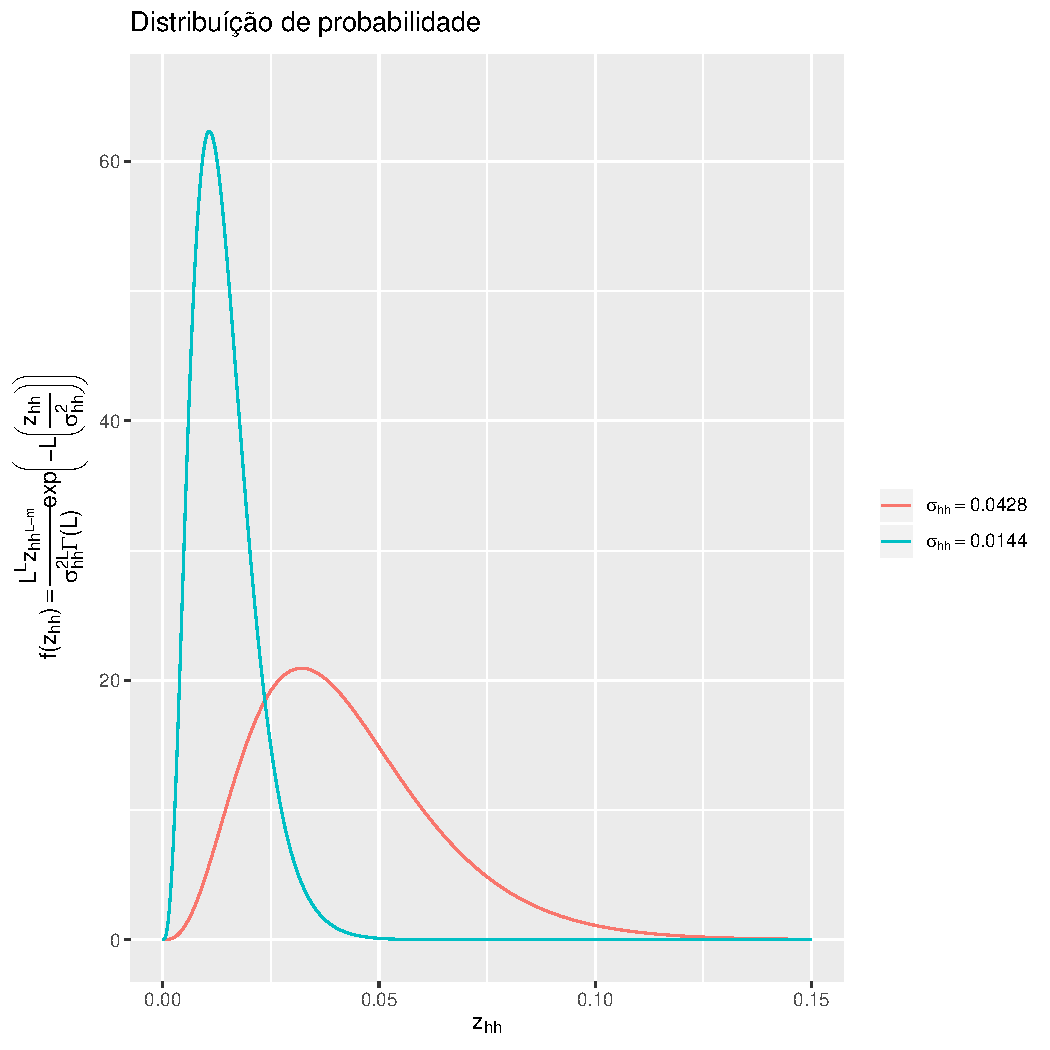
\includegraphics[scale = 1]{grafico_pdf_gamf_2017_sigma_hh.pdf}
  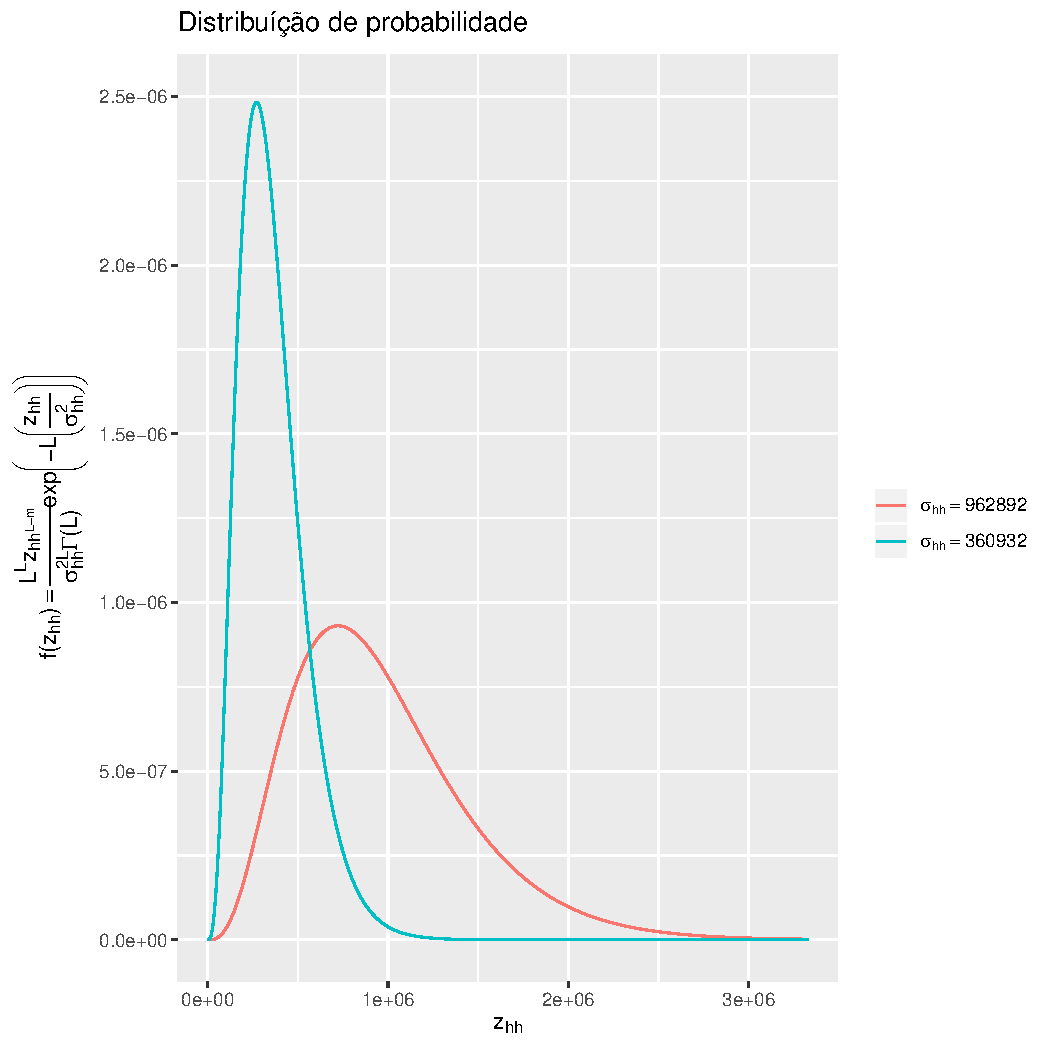
\includegraphics[scale = 0.7]{grafico_pdf_nhfc_2014_sigma_hh.pdf}
	\caption{Funções de densidade para dados simulados.}\label{cap_acf_fig02}
\end{figure}
%%% ACF Para fins de comparação, seria interessante ver as densidades no mesmo gráfico

A figura (\ref{cap_acf_fig01}) foi gerada com auxílio das distribuições Wishart descritas nas equações (\ref{cap_acf_13}) para $L=4$ e matrizes de covariância com $\Sigma_{u}$ e $\Sigma_{f}$ definidos em (\ref{cap_acf_24}) e (\ref{cap_acf_25}).
	
A imagem de fato é construída com $400$ linhas distribuídas em duas bandas separadas verticalmente em torno do pixel $200$, lembrando que a imagem tem dimensão $400 \times 400$. Cada linha  tem duas amostras diferentes geradas com os parâmetros $\Sigma_{u}$ e $\Sigma_{f}$ respectivamente e ainda $L=4$ para as duas amostras.  

	O valor $200$ é fixado horizontalmente para termos uma linha contendo as duas amostras, para essa linha é calculado $l(j)$ conforme equação (\ref{cap_acf_21}) que deve ser aplicada nos canais $\mathbf{I_{hh}}$, $\mathbf{I_{vh}}$ e $\mathbf{I_{vv}}$.  
\begin{figure}[hbt]
\minipage{0.5\textwidth}
  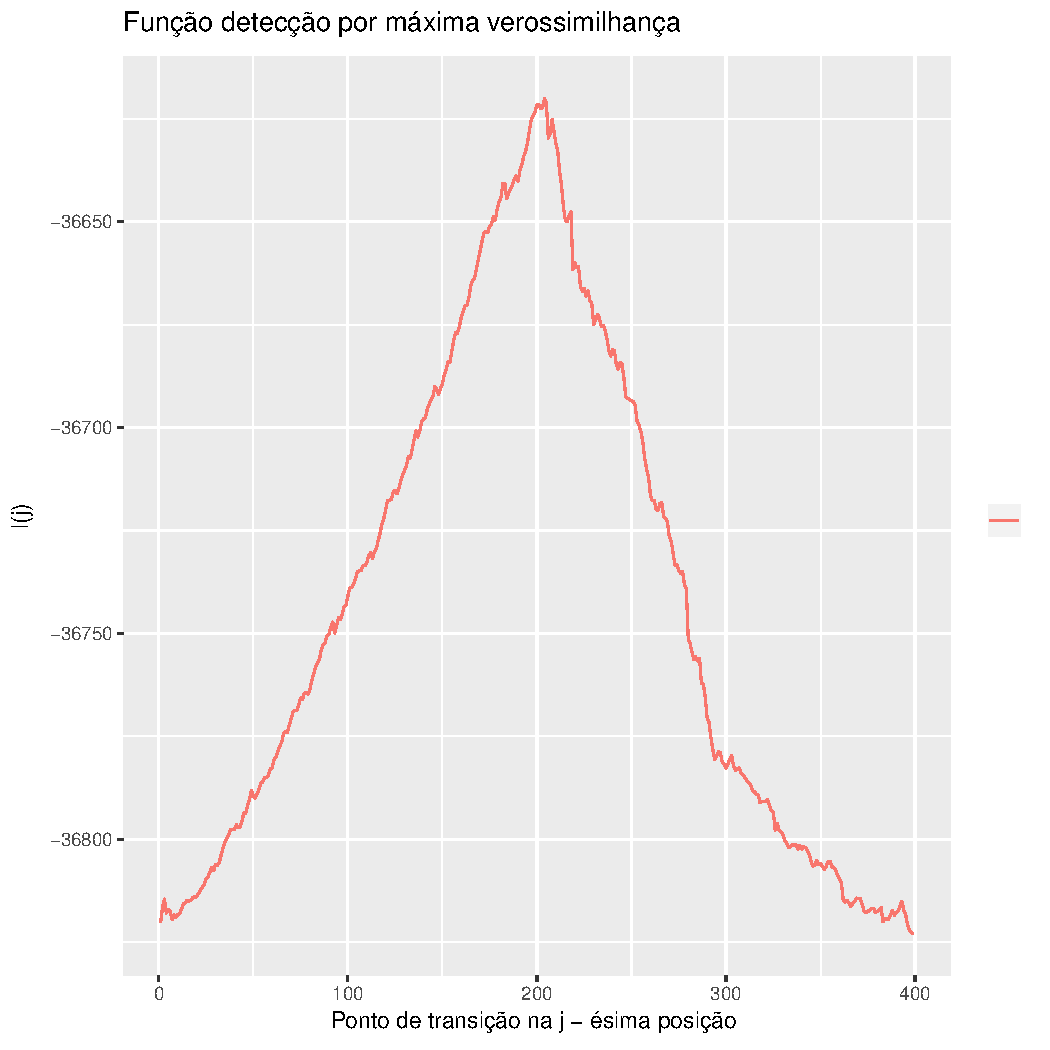
\includegraphics[width=\linewidth]{grafico_l_nhfc_2014_sigmahh.pdf}
	\caption{Função $l(j)$ para o canal $I_{HH}$}\label{cap_acf_fig04}
\endminipage\hfill
\minipage{0.5\textwidth}
  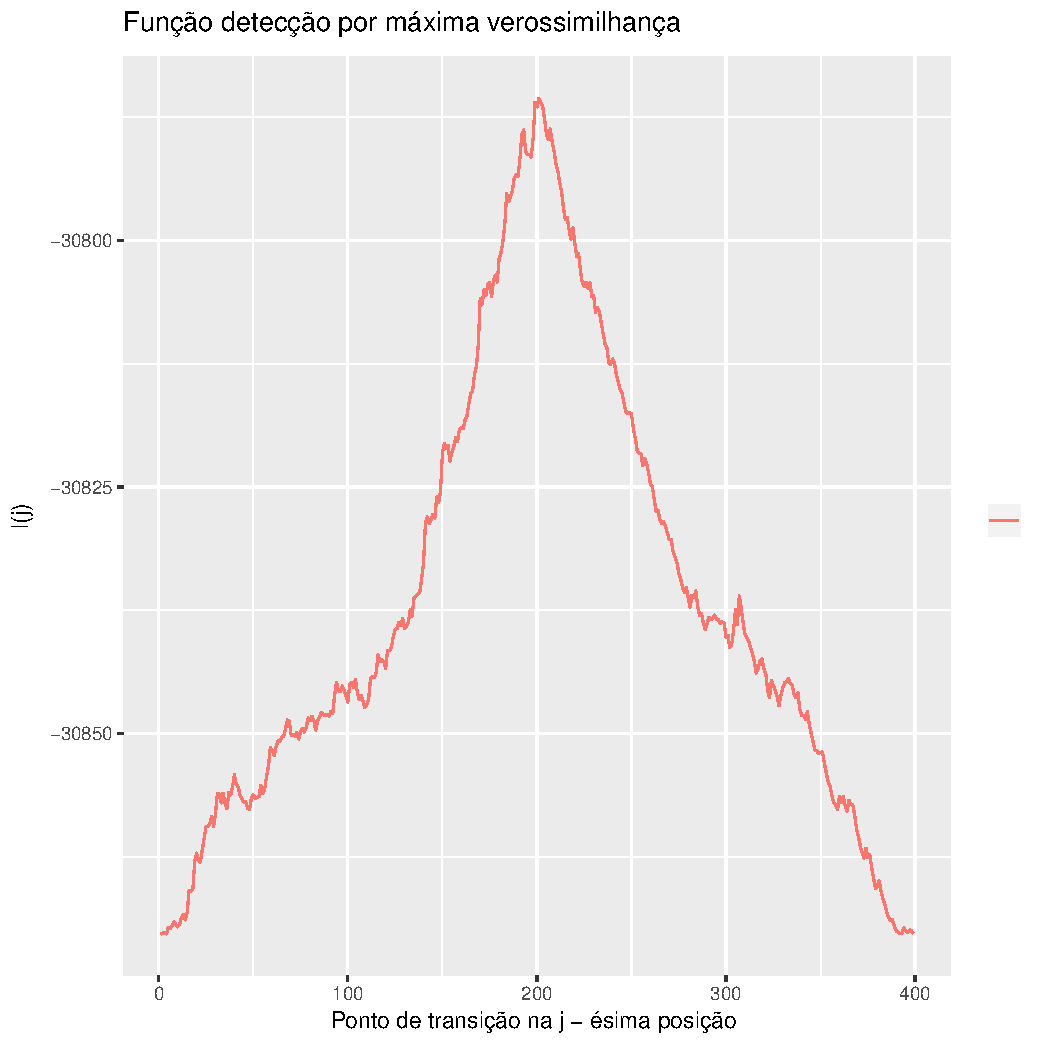
\includegraphics[width=\linewidth]{grafico_l_nhfc_2014_sigmahv.pdf}
	\caption{Função $l(j)$ para o canal $I_{HV}$}\label{cap_acf_fig05}
\endminipage\hfill
\centering
\minipage{0.5\textwidth}
  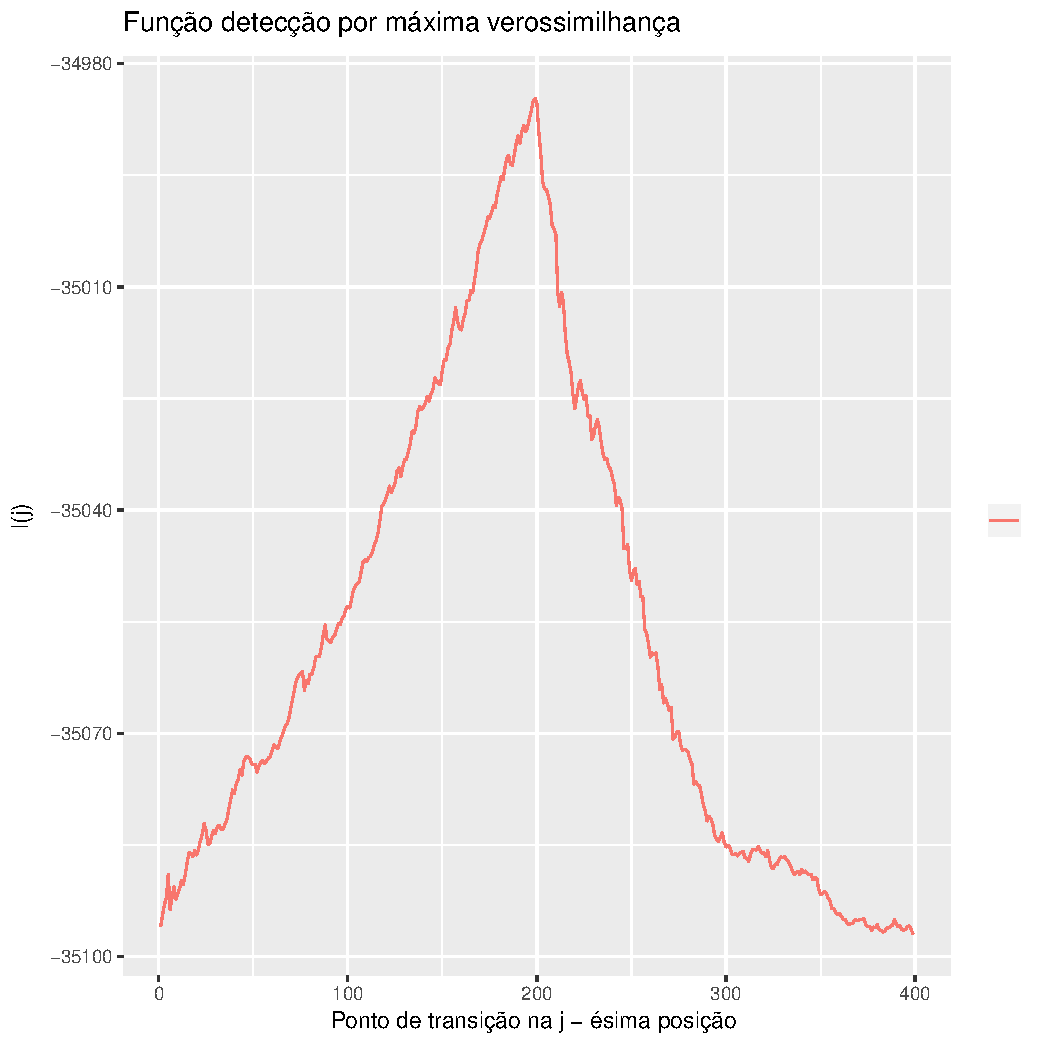
\includegraphics[width=\linewidth]{grafico_l_nhfc_2014_sigmavv.pdf}
	\caption{Função $l(j)$ para o canal $I_{VV}$}\label{cap_acf_fig06}
\endminipage\hfill
\end{figure}

	Podemos notar que as funções não são deriváveis em muitos pontos, então os métodos de otimização que necessitam do cálculo da derivada, terão funcionamento comprometido, resolvemos esse problema usando o método Simulated Anneling Generalizado (GenSA) que podemos encontrar na referência \citep{xgsh}.
	
	O método GenSA mostrou-se competitivo com os métodos empregados no artigo \citet{nhfc}, para testar a acurácia do GenSA e fazer a comparação com os métodos aplicados no artigo, vamos usar a métrica encontrada no artigo \citep{nhfc} e proposta na referência \citep{fbgm}.
        
	O erro foi calculado gerando $400$ replicações da distribuição Wishart com duas amostras como acima, gerando uma função $l(j)$ para cada replicação. Aplicando o GenSA para cada umas das $l(j)$ temos as evidências de bordas ou pontos de transição. O ponto de borda é $200$ por construção para todas as replicações, então o erro para cada replicação é o valor absoluto da diferença entre o ponto de borda e o valor estimado pelo método GenSA, portanto  
\begin{equation}\label{cap_acf_26}
\begin{array}{llll}
	E(r) &=& |200 - \hat{\jmath}(r)|, & 1\leq r \leq 400,  \\
\end{array}
\end{equation}
onde, $\hat{\jmath}(r)$ é o resultado da maximização de $l(j)$ pelo método GenSA na replicação $r$.

Usaremos frequências relativas para estimar a probabilidade de ter um erro menor que um número de pixeis. Denotando por $H(k)$ o número de replicações para qual o erro é menor que $k$ pixeis, então calculamos uma estimativa desta probabilidade por $f(k)=\frac{H(k)}{400}$. Nos testes realizados nesta seção variamos $k$ entre $1$ e $10$. O algoritmo está descrito em detalhes na referência \citep{fbgm}. 
\begin{figure}[hbt]
\minipage{0.475\textwidth}
\fbox{  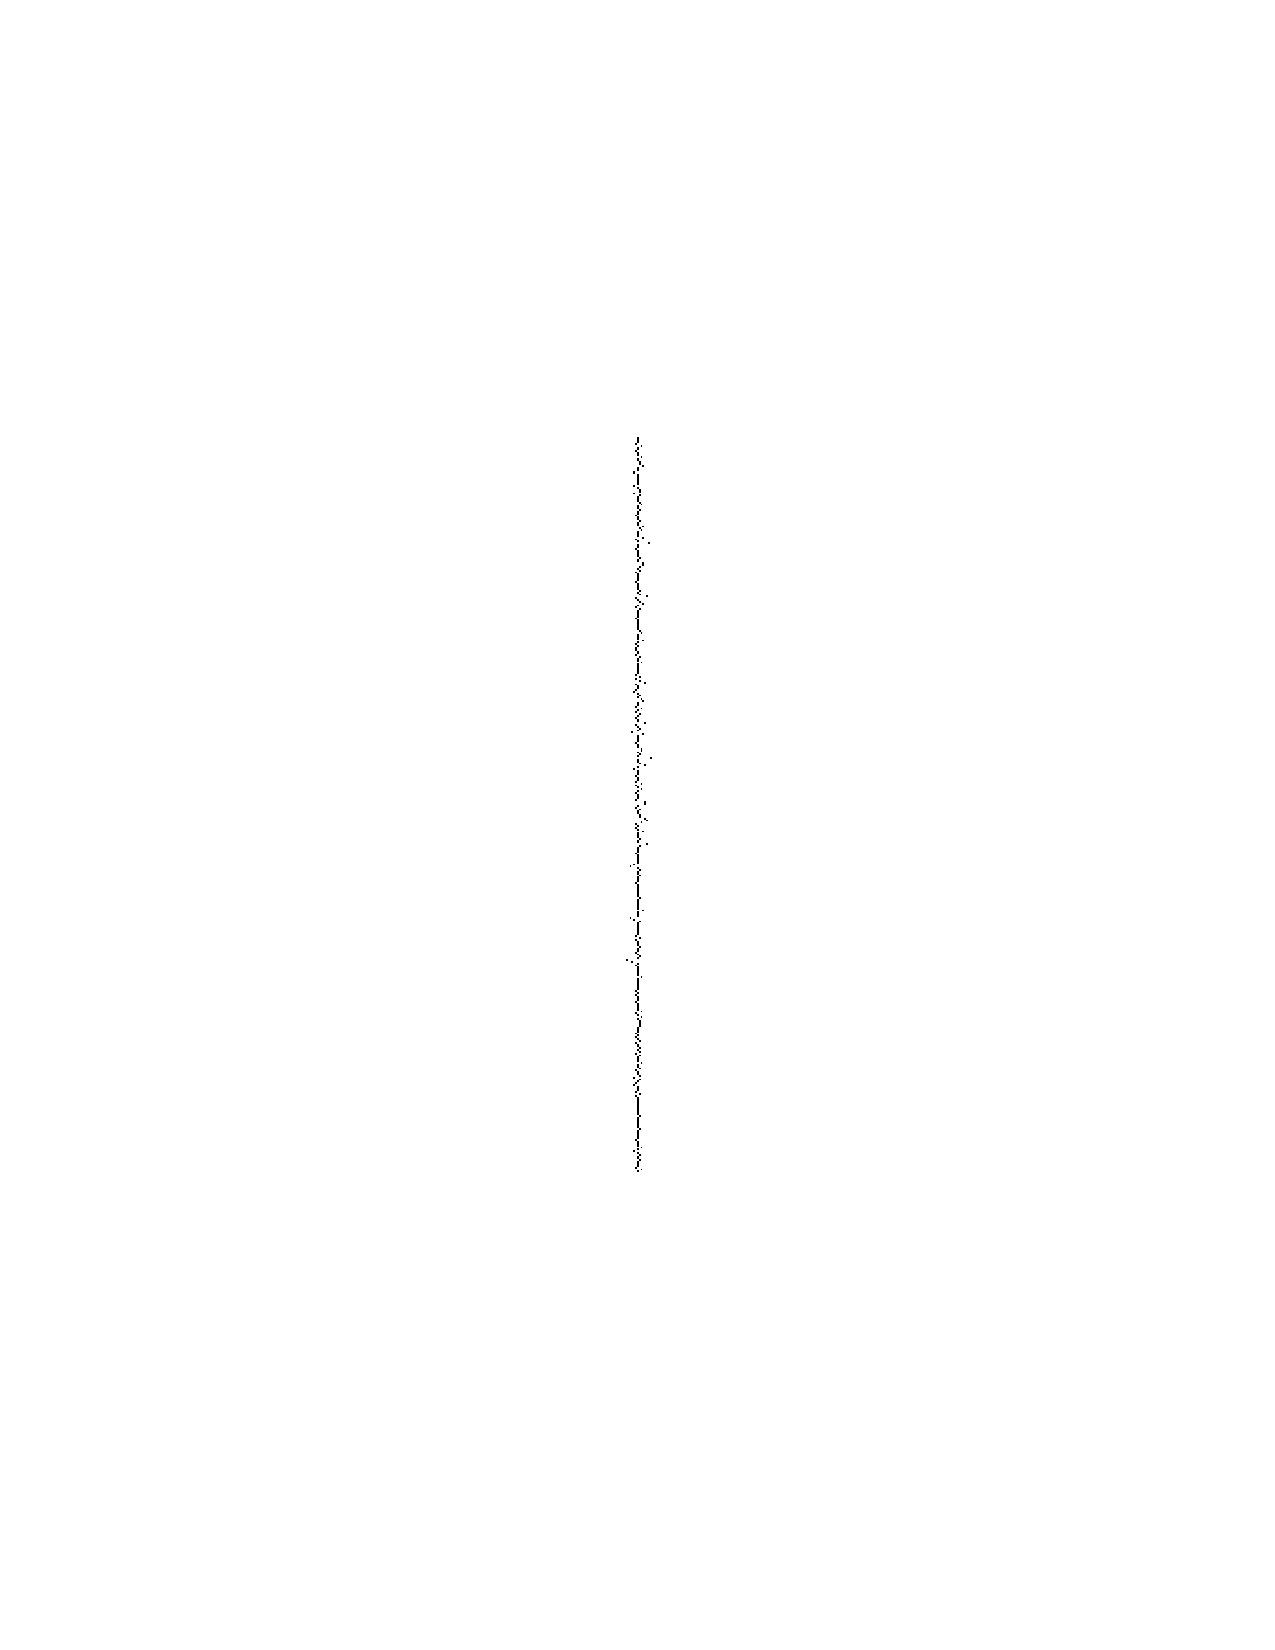
\includegraphics[width=\linewidth]{ev_hh_nhfc_2014.pdf}}
\caption{Evidências de bordas para o canal $I_{HH}$}\label{cap_acf_fig07}
\endminipage\hfill
\minipage{0.475\textwidth}
\fbox{ 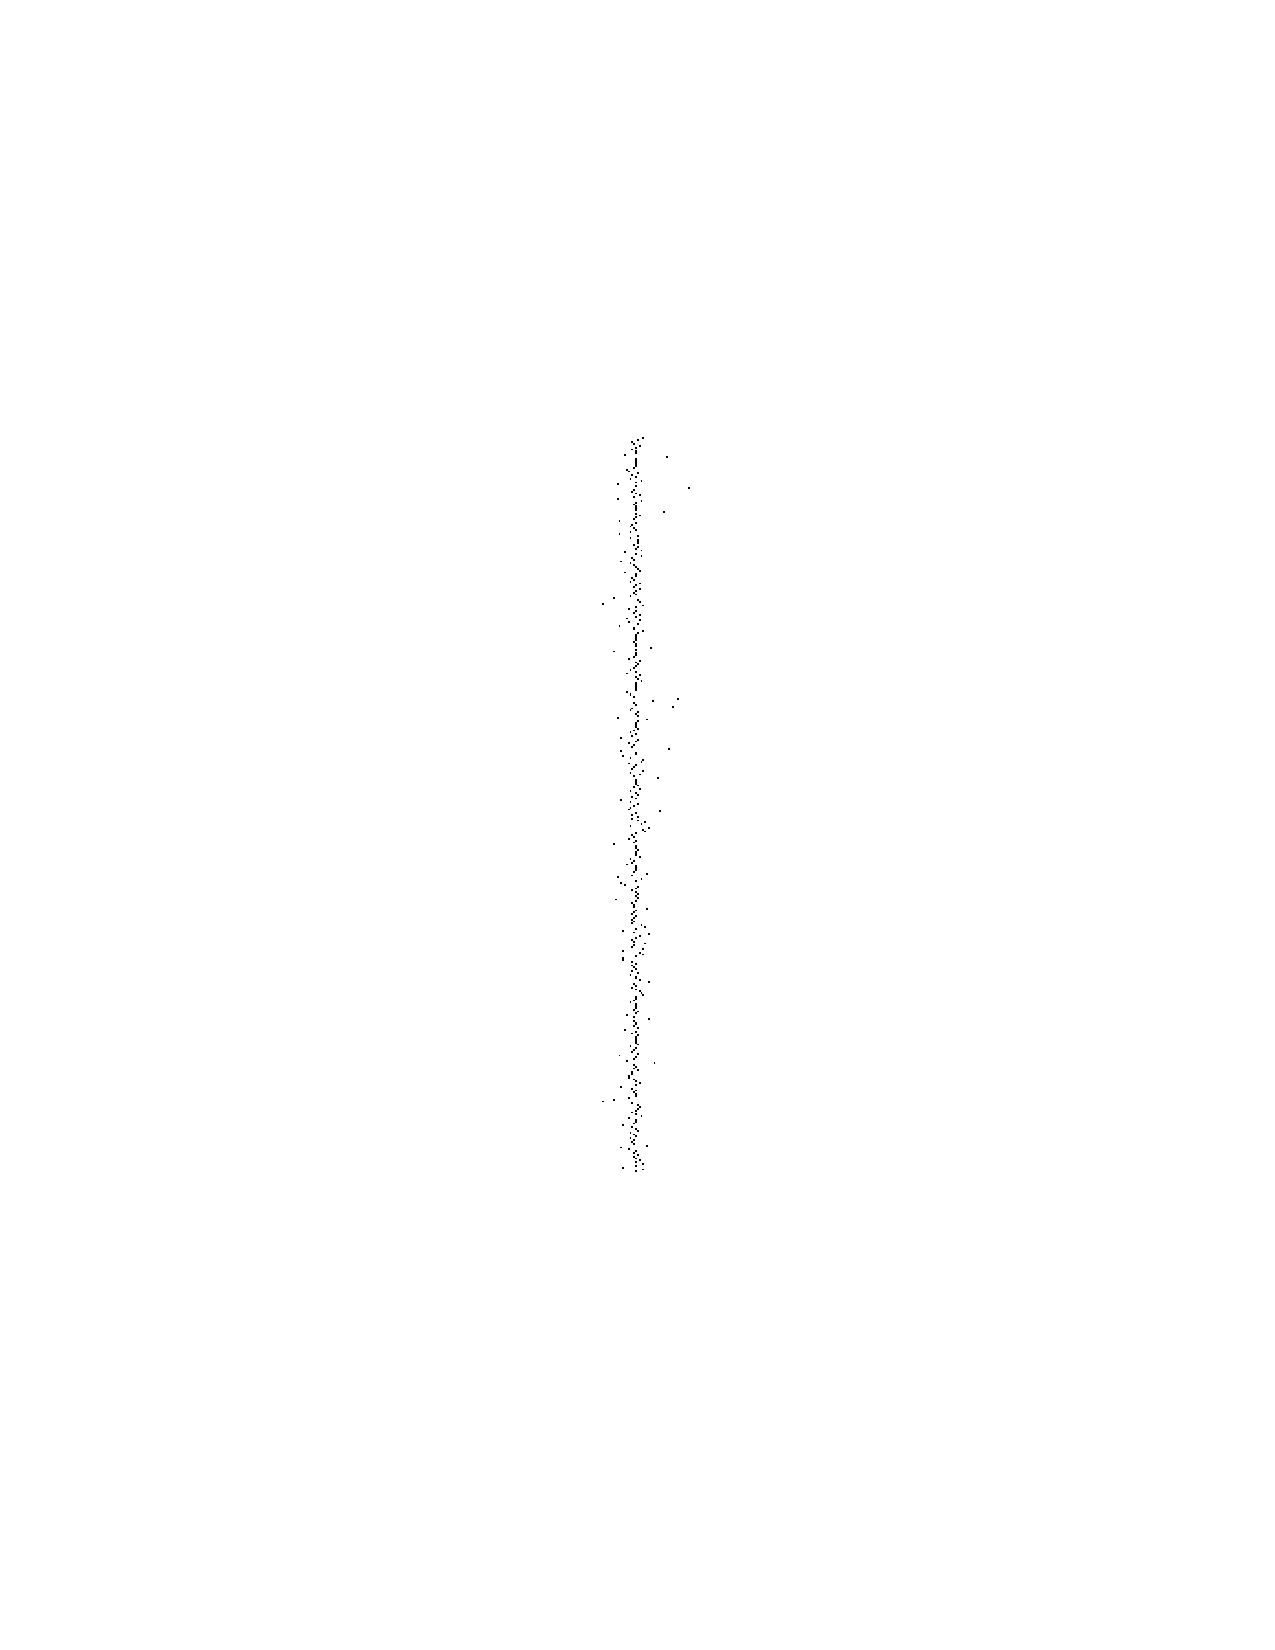
\includegraphics[width=\linewidth]{ev_hv_nhfc_2014.pdf}}
\caption{Evidências de bordas para o canal $I_{HV}$}\label{cap_acf_fig08}
\endminipage\hfill
\centering
\minipage{0.475\textwidth}
\fbox{ 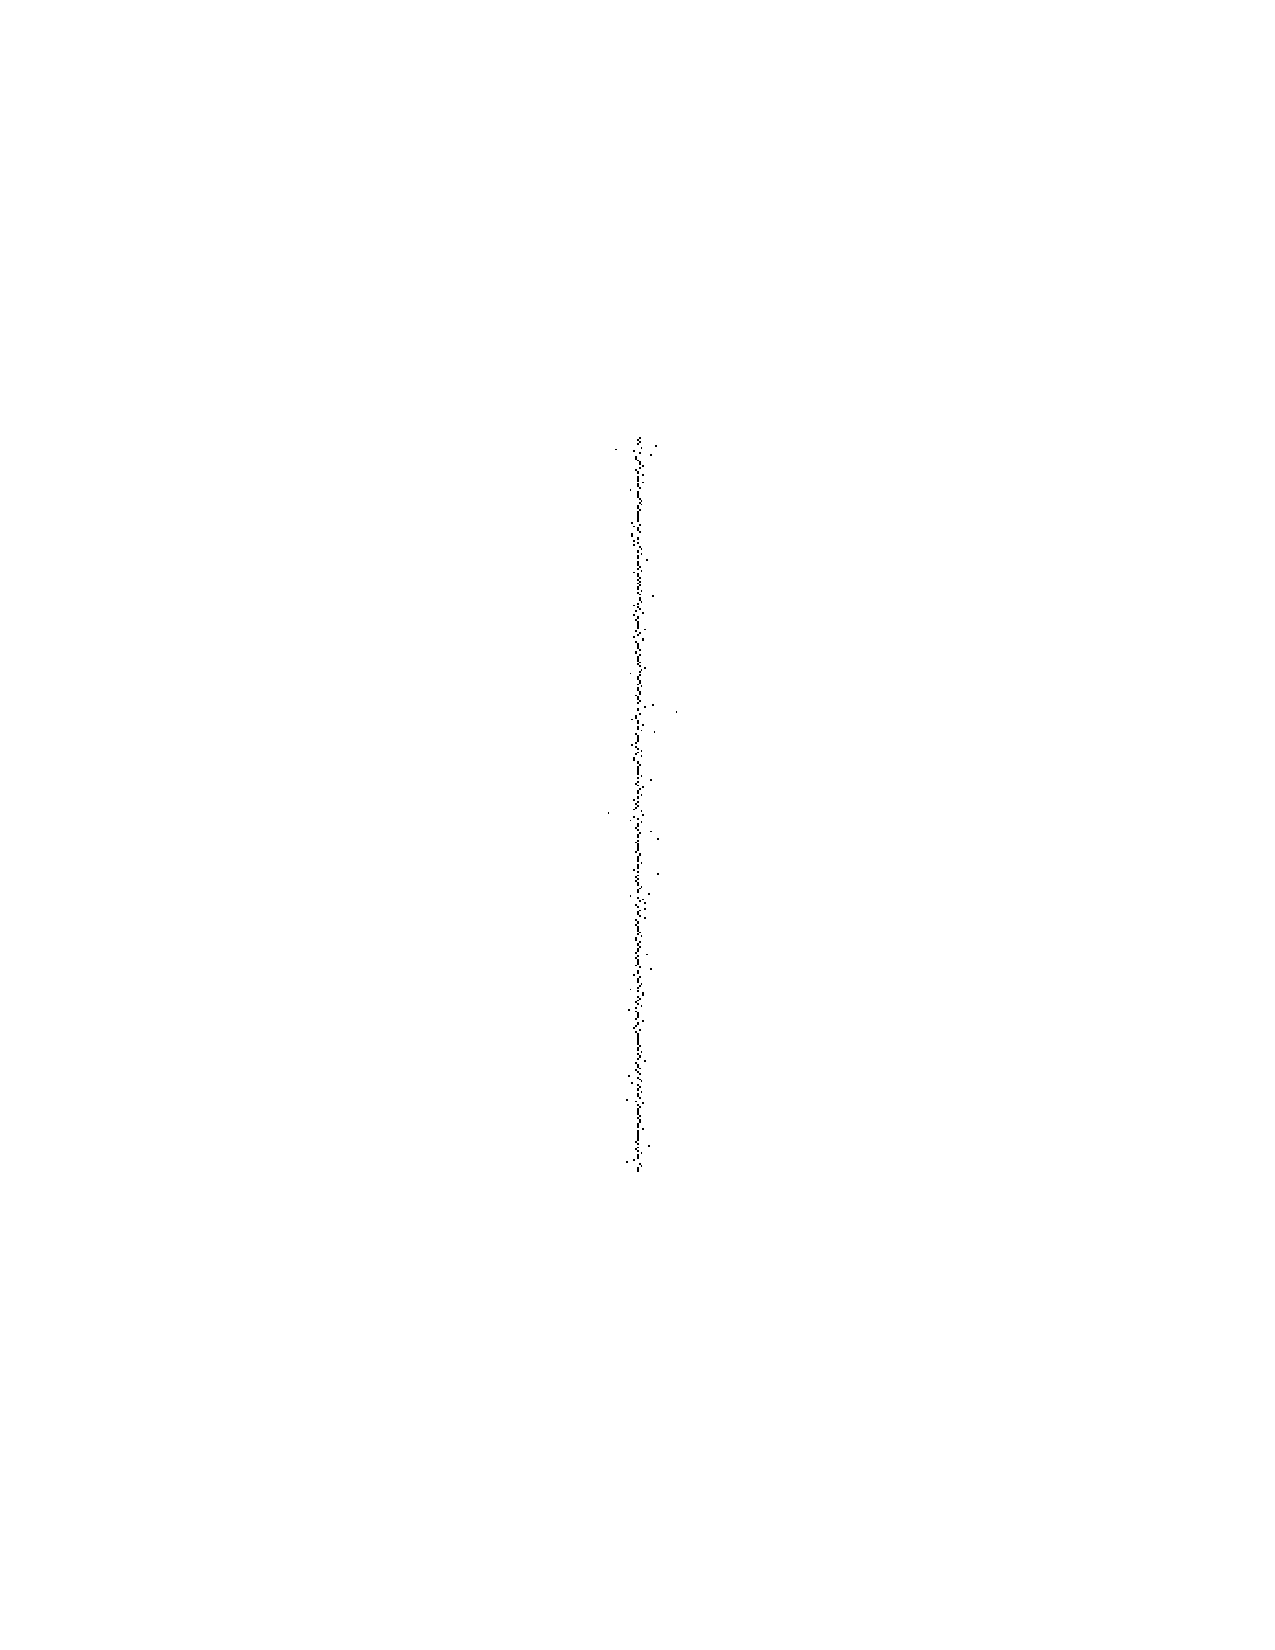
\includegraphics[width=\linewidth]{ev_vv_nhfc_2014.pdf}}
\caption{Evidências de bordas para o canal $I_{VV}$}\label{cap_acf_fig09}
\endminipage\hfill
\end{figure}

	A figura (\ref{cap_acf_fig10}) mostra as probabilidades para a detecção de bordas quando aplicado o método GenSA nos canais $I_{hh}$, $I_{vh}$ e $I_{vv}$ da imagem mostrada na figura (\ref{cap_acf_fig01}). As 400 replicações para cada canal e sua respectiva evidência de borda estão nas figuras (\ref{cap_acf_fig07}),(\ref{cap_acf_fig08}) e (\ref{cap_acf_fig09}).  
\begin{figure}[hbt]
\centering
	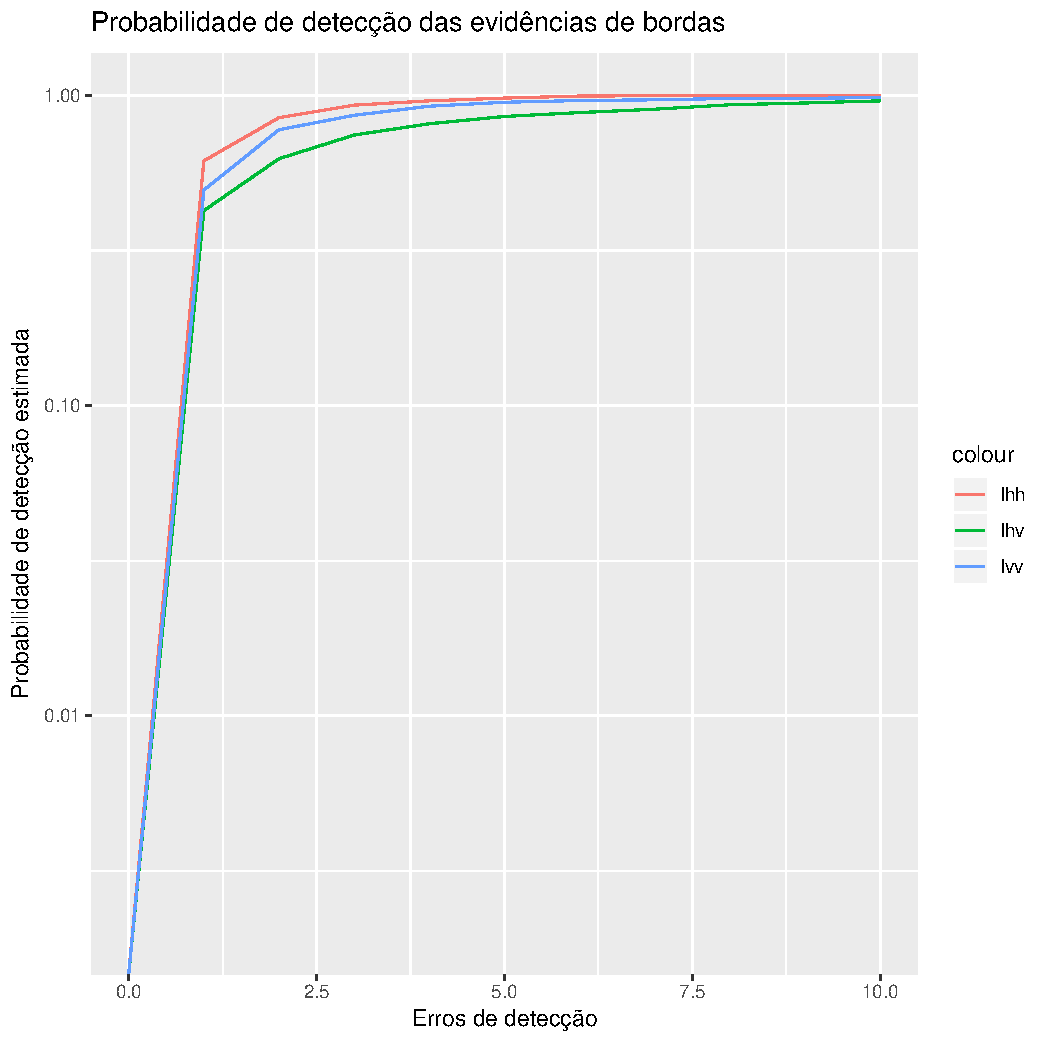
\includegraphics[width=5.0in]{metricas_ihh_ivh_ivv_nhfc.pdf}
	\caption{Probabilidade de detecção de borda estimada usando GenSA.}
\label{cap_acf_fig10}
\end{figure}

\section{Fusão de evidências de bordas}

	Nesta seção será descrito como realizamos a fusão de evidências de bordas, a referência adotada foi \citet{mit} que mostra várias técnicas de fusão de imagens. 

	Sejam $I_k(m,n)$, com $k=1,2,\cdots,K$ imagens provenientes da detecção de bordas após a aplicação do método GenSA com dimensões $m \times n$, podemos definir a estratégia de fusão de evidências da seguinte forma, seja o índice $k$ variando como $k=\{hh,vh,vv\}$, para cada linha das imagens e para os respectivos canais $I_k$ temos um valor de evidências de bordas.  Os mesmos serão armazenados em um vetor denotado $ev_k$ com índices variando como $k=\{hh,vh,vv\}$ e dimensão $m$, assim a fusão de evidências $F_{m}^{ev}$ é definida como,
\begin{equation}\label{cap_acf_27}
\begin{array}{lll}
	F_{m}^{ev} &=&\frac{1}{K}\sum_{k=1}^{K}ev_k  \\
\end{array}
\end{equation}
 O resultado da técnica de fusão de evidências é mostrado na figura (\ref{cap_acf_fig11}).

Com o intuito de melhorar a detecção de borda propomos aplicar o método de quadrados mínimos (\textbf{MMQ}) nos dados da fusão de evidências, realizando essa aplicação temos o resultado do método dos quadrados mínimos junto com os pontos de fusão de evidências, mostrados na figura (\ref{cap_acf_fig12}).
\begin{figure}[hbt]
\minipage{0.475\textwidth}
	\fbox{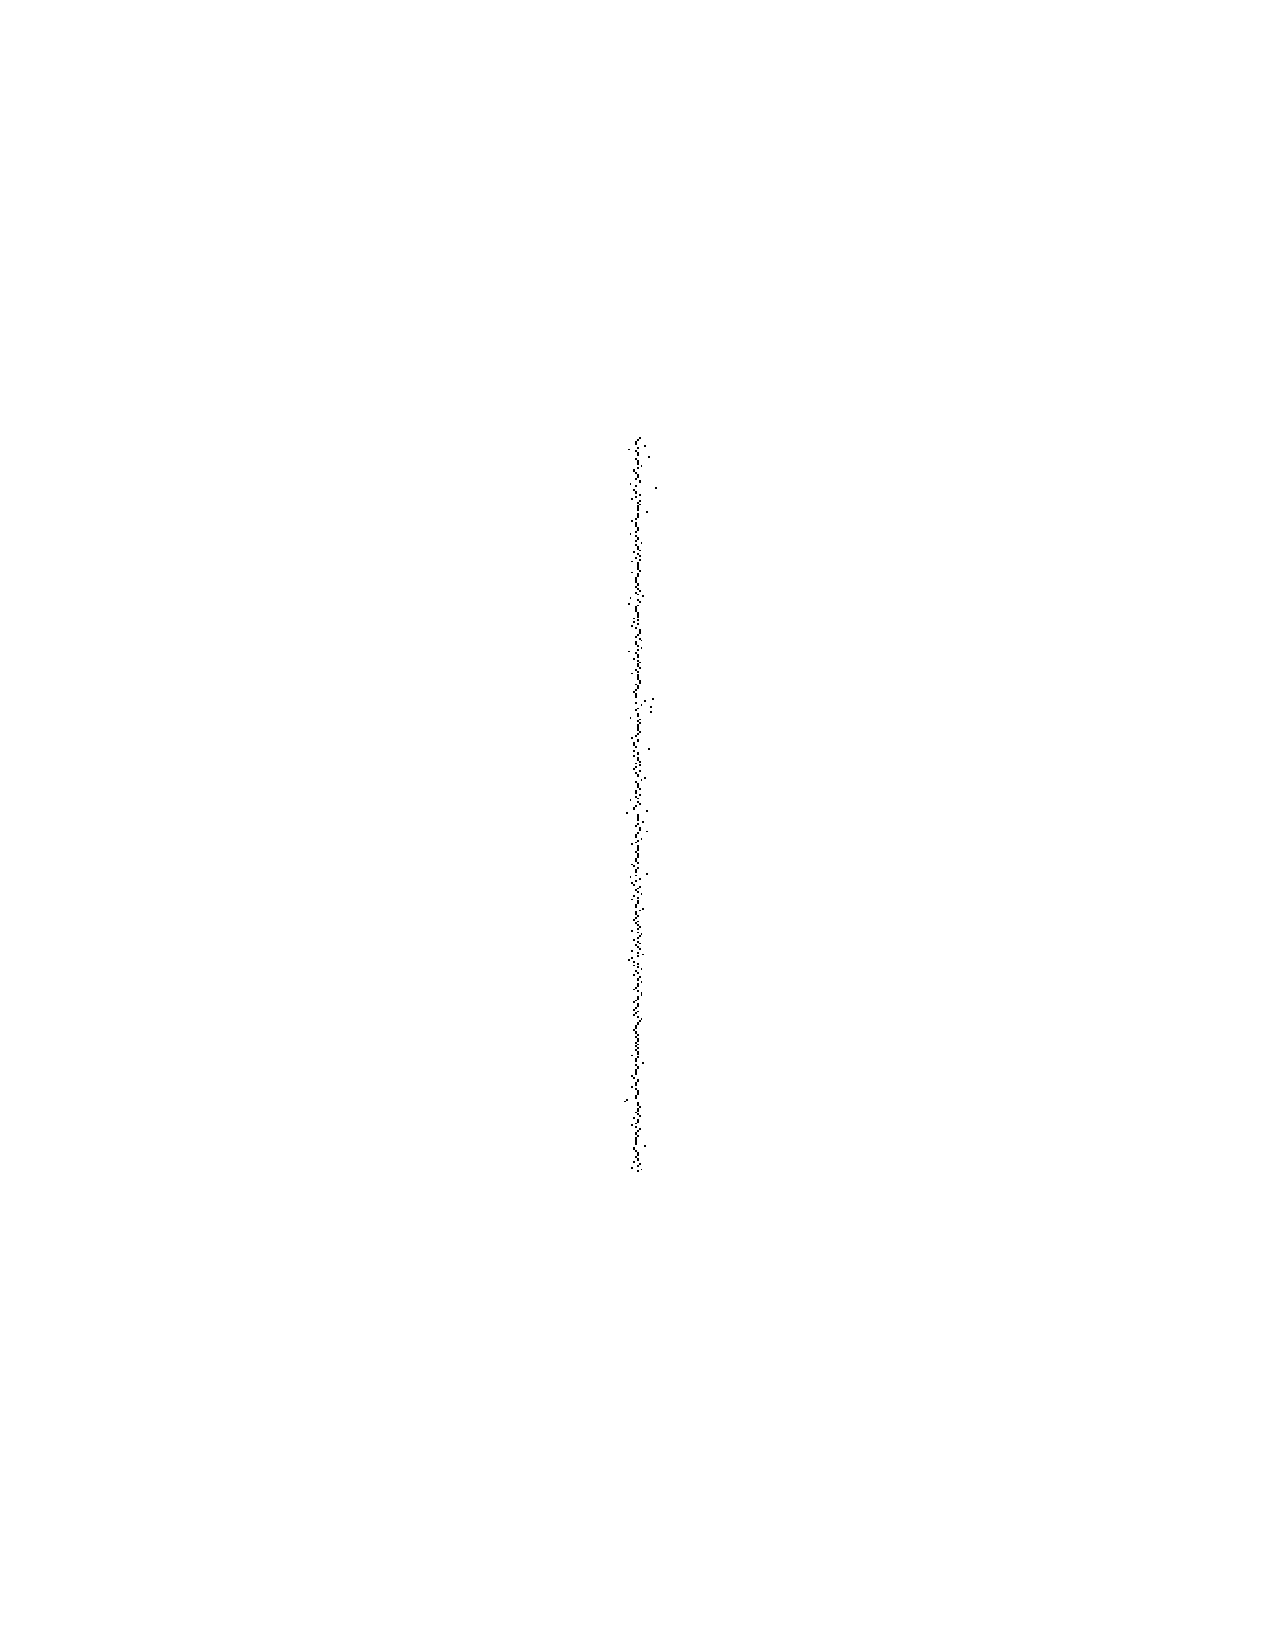
\includegraphics[width=\linewidth]{fusao_soma_ev_hh_hv_vv_nhfc.pdf}}
	\caption{Fusão de evidências para os canais $\left(I_{hh}, I_{hv}, I_{vv}\right)$.}
\label{cap_acf_fig11}
\endminipage\hfill
\minipage{0.475\textwidth}
\fbox{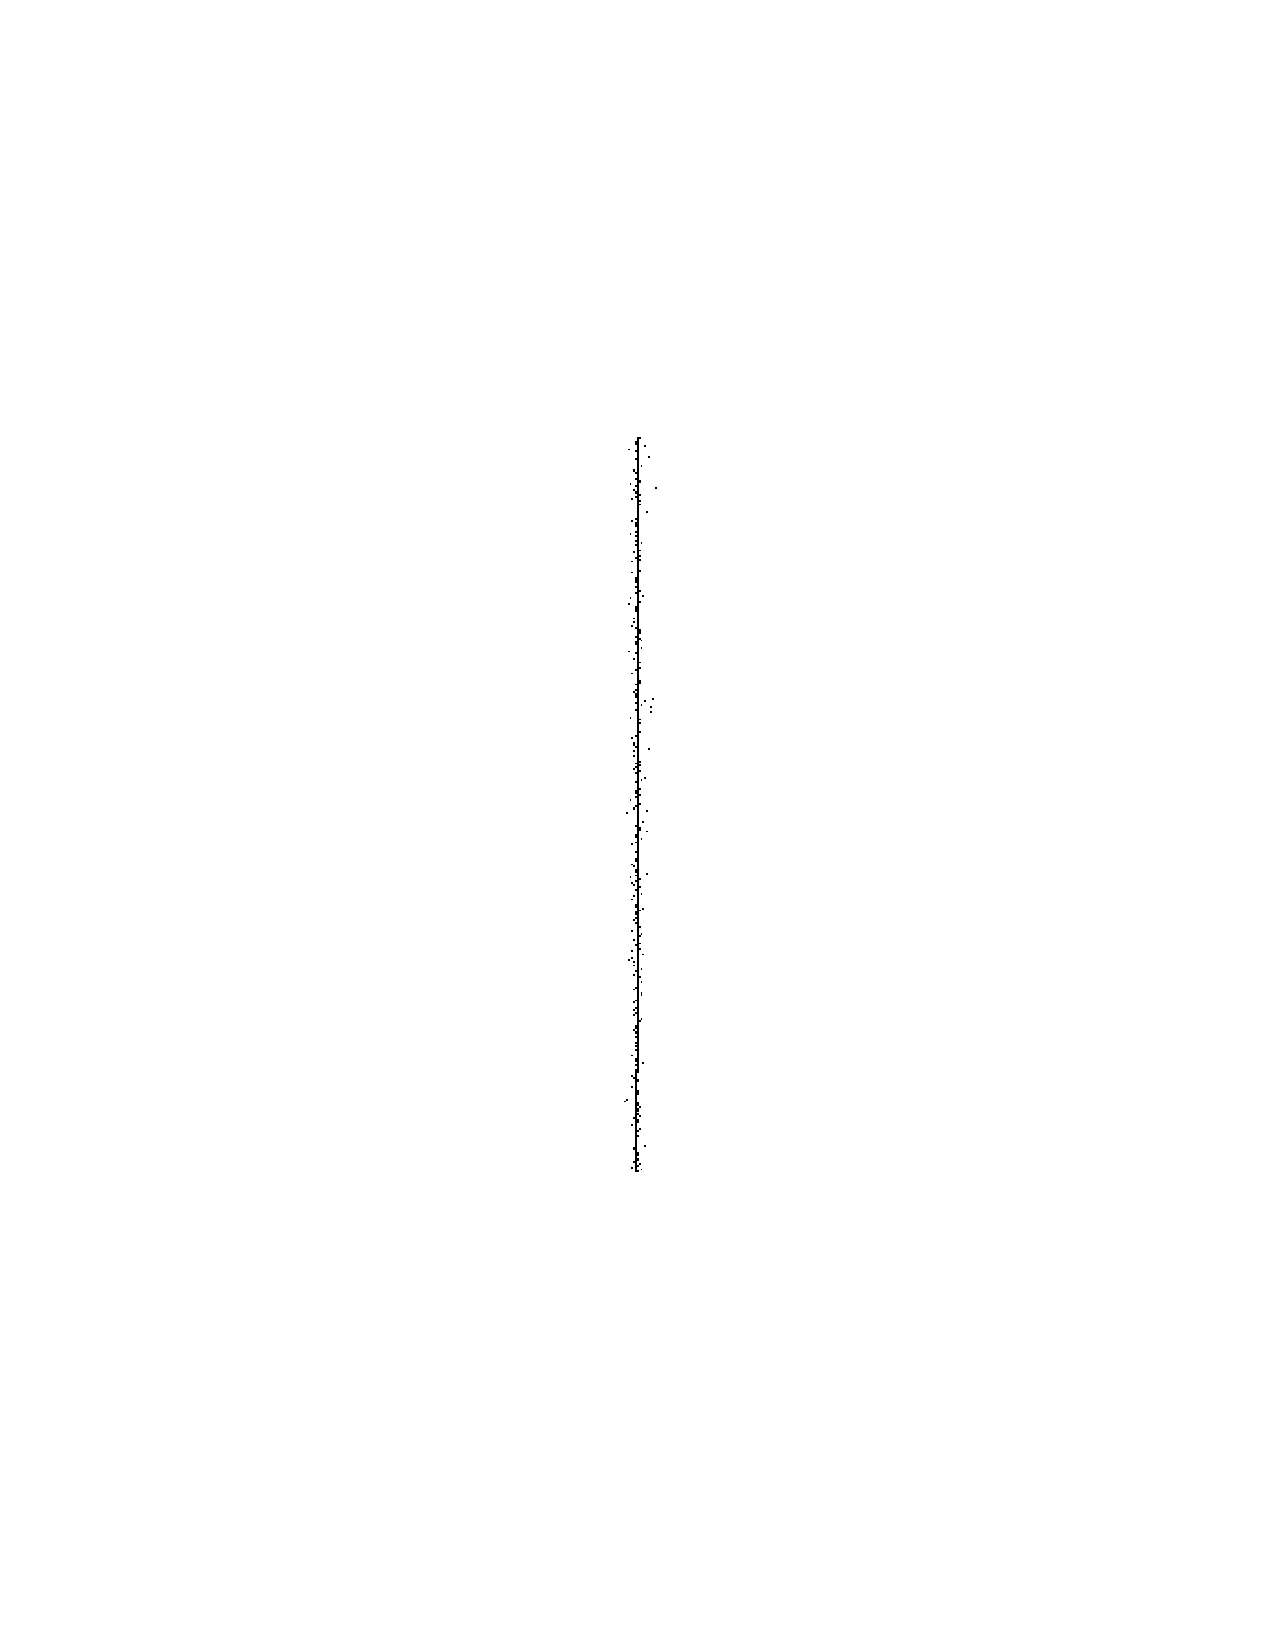
\includegraphics[width=\linewidth]{fusao_ls_nhfc.pdf}}	
\caption{Método dos quadrados mínimos aplicado a fusão de imagens.}
\label{cap_acf_fig12}
\endminipage\hfill
\end{figure}
Observando a figura podemos notar um bom desempenho da aplicação do método dos quadrados mínimos nos dados provenientes da fusão de evidências. Para confirmar a observação vamos calcular a frequência relativa desse método, a qual mostra a probabilidade de detecção de borda estimada como na figura (\ref{cap_acf_fig10}).
\begin{figure}[hbt]
\minipage{0.475\textwidth}
	\fbox{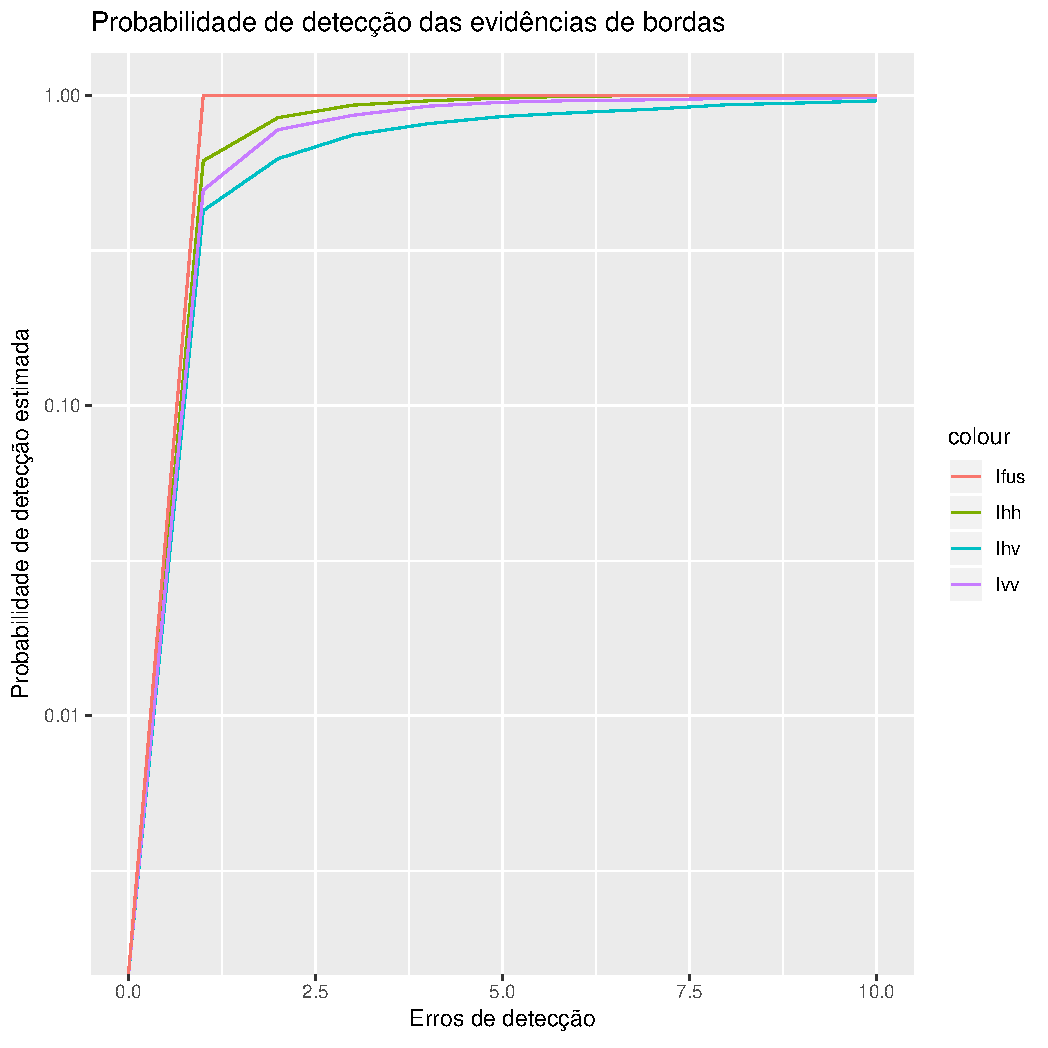
\includegraphics[width=\linewidth]{metricas_ihh_ivh_ivv_ils_nhfc.pdf}}
	\caption{Probabilidade de detecção de borda com fusão de evidências.}
\label{cap_acf_fig13}
\endminipage\hfill
\minipage{0.475\textwidth}
\fbox{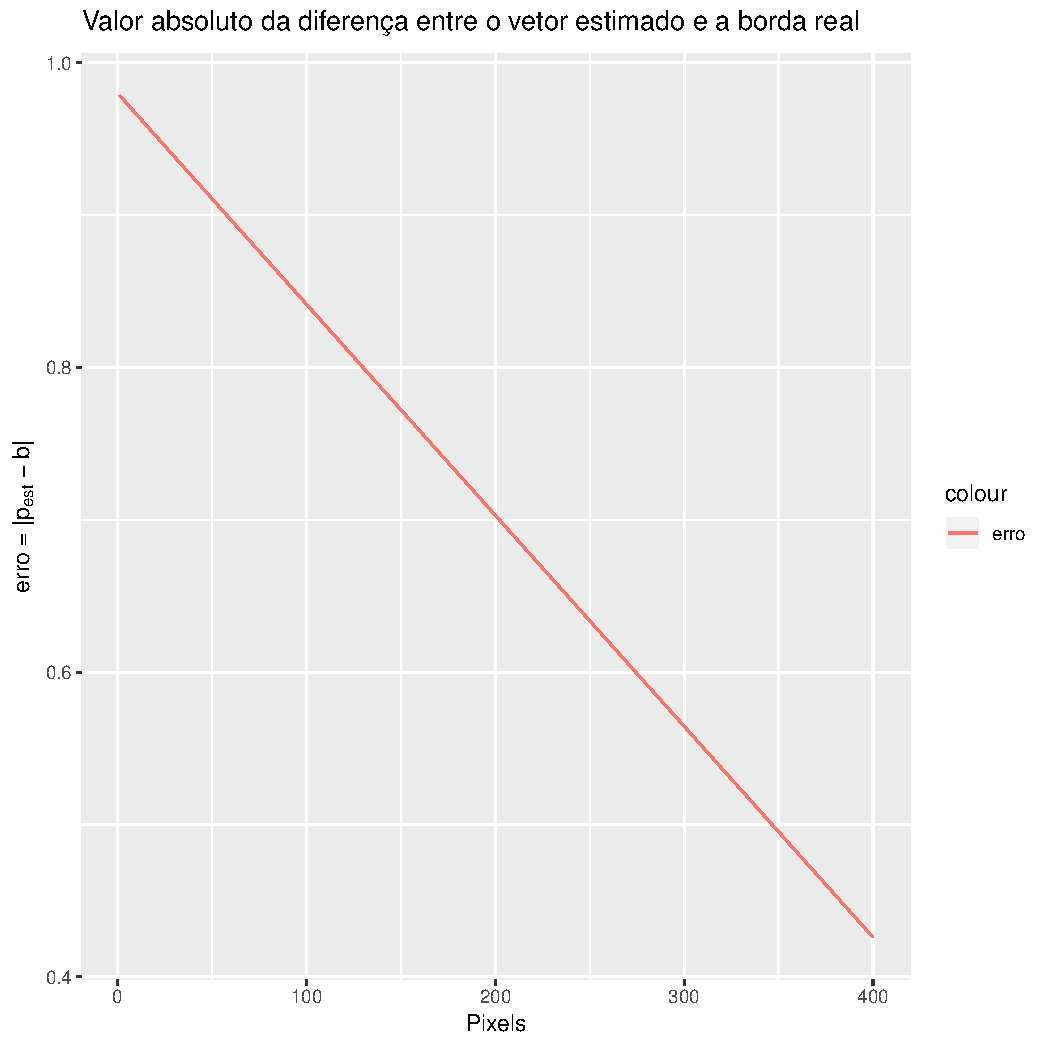
\includegraphics[width=\linewidth]{fusao_ls_erro_nhfc.pdf}}	
	\caption{Valor absoluto da diferença entre o vetor estimado da fusão de evidências e a borda real.}
\label{cap_acf_fig14}
\endminipage\hfill
\end{figure}

A figura (\ref{cap_acf_fig13}) mostra a frequência relativa para a fusão de evidências, juntamente com a frequência relativa de detecção de bordas, nos respectivos canais. O gráfico foi construído para notarmos o bom desempenho do método de fusão e posterior aplicação do método dos quadrados mínimos. Desta forma podemos ver que a probabilidade de detecção para o método proposto alcança melhores resultados em relação as detecções em cada canal. 

 Definindo o vetor $P_{est}$ como sendo o vetor de tamanho $400$, tal que, suas componentes são as bordas estimadas pelo método proposto. O vetor $b$ é definido com o valor de borda igual a $200$ para todas as componentes. O gráfico da figura (\ref{cap_acf_fig14}) mostra o $erro=|P_{est}-b|$ para cada pixel que o método foi aplicado, e o máximo atingido do erro foi $erro=0.8162$, isto é, a acurácia do método é menor que um pixel, confirmando o resultado mostrado na figura (\ref{cap_acf_13}).

A ideia proposta de aplicar o método GenSA para estimar as evidências de bordas juntamente com os métodos de fusão de evidências e quadrados  mínimos (\textbf{MMQ}) teve um desempenho superior na detecção de bordas em relação a detecção nos respectivos canais, como mostra a figura (\ref{cap_acf_fig13}) e (\ref{cap_acf_fig14}). Podemos concluir que para a imagem simulada o método possui uma acurácia satisfatória para a detecção de bordas.
\chapter{Objetivos}
Com o propósito de buscar por outros e melhores resultados foram traçados os seguintes objetivos: 
\begin{itemize}
    \item[1-] propor e analisar outras técnicas de fusão de evidências (dezembro   2018); 
	\item[2-] Aplicar o método em uma imagem real para analisar o seu desempenho e acurácia da borda encontrada (março 2019);
	\item[3-] Propor e analisar outras técnicas de regressão ou classificação como por exemplo Support Vector Machine $(SVM)$, ou Randon Forest $(RF)$ para  comparar com o método de quadrados mínimos usado neste texto (março 2019);
	\item[4-] Aplicar um filtro tipo borrador na função $l(j)$ com intuito de melhorar sua suavidade facilitando o cálculo do gradiente e consequentemente comparar métodos clássicos de otimização com a aplicação do método GenSA proposto neste trabalho (dezembro 2018). 
\end{itemize}

Propostas para \textit{workshops}, congressos e publicações:
\begin{itemize}
\item participar do \textit{workshop} semestral promovido pelo programa de pós-graduação em engenharia elétrica e computação (dezembro 2018);
\item finalizar um artigo para publicar em congresso de relevância internacional (dezembro 2018);
\item finalizar um artigo para publicar em revista internacional avaliada de acordo com a área de atuação (março 2019);
\end{itemize}
\chapter{Testes numéricos}
\section{Sigmas do artigo }
\begin{figure}[hbt]
\centering
	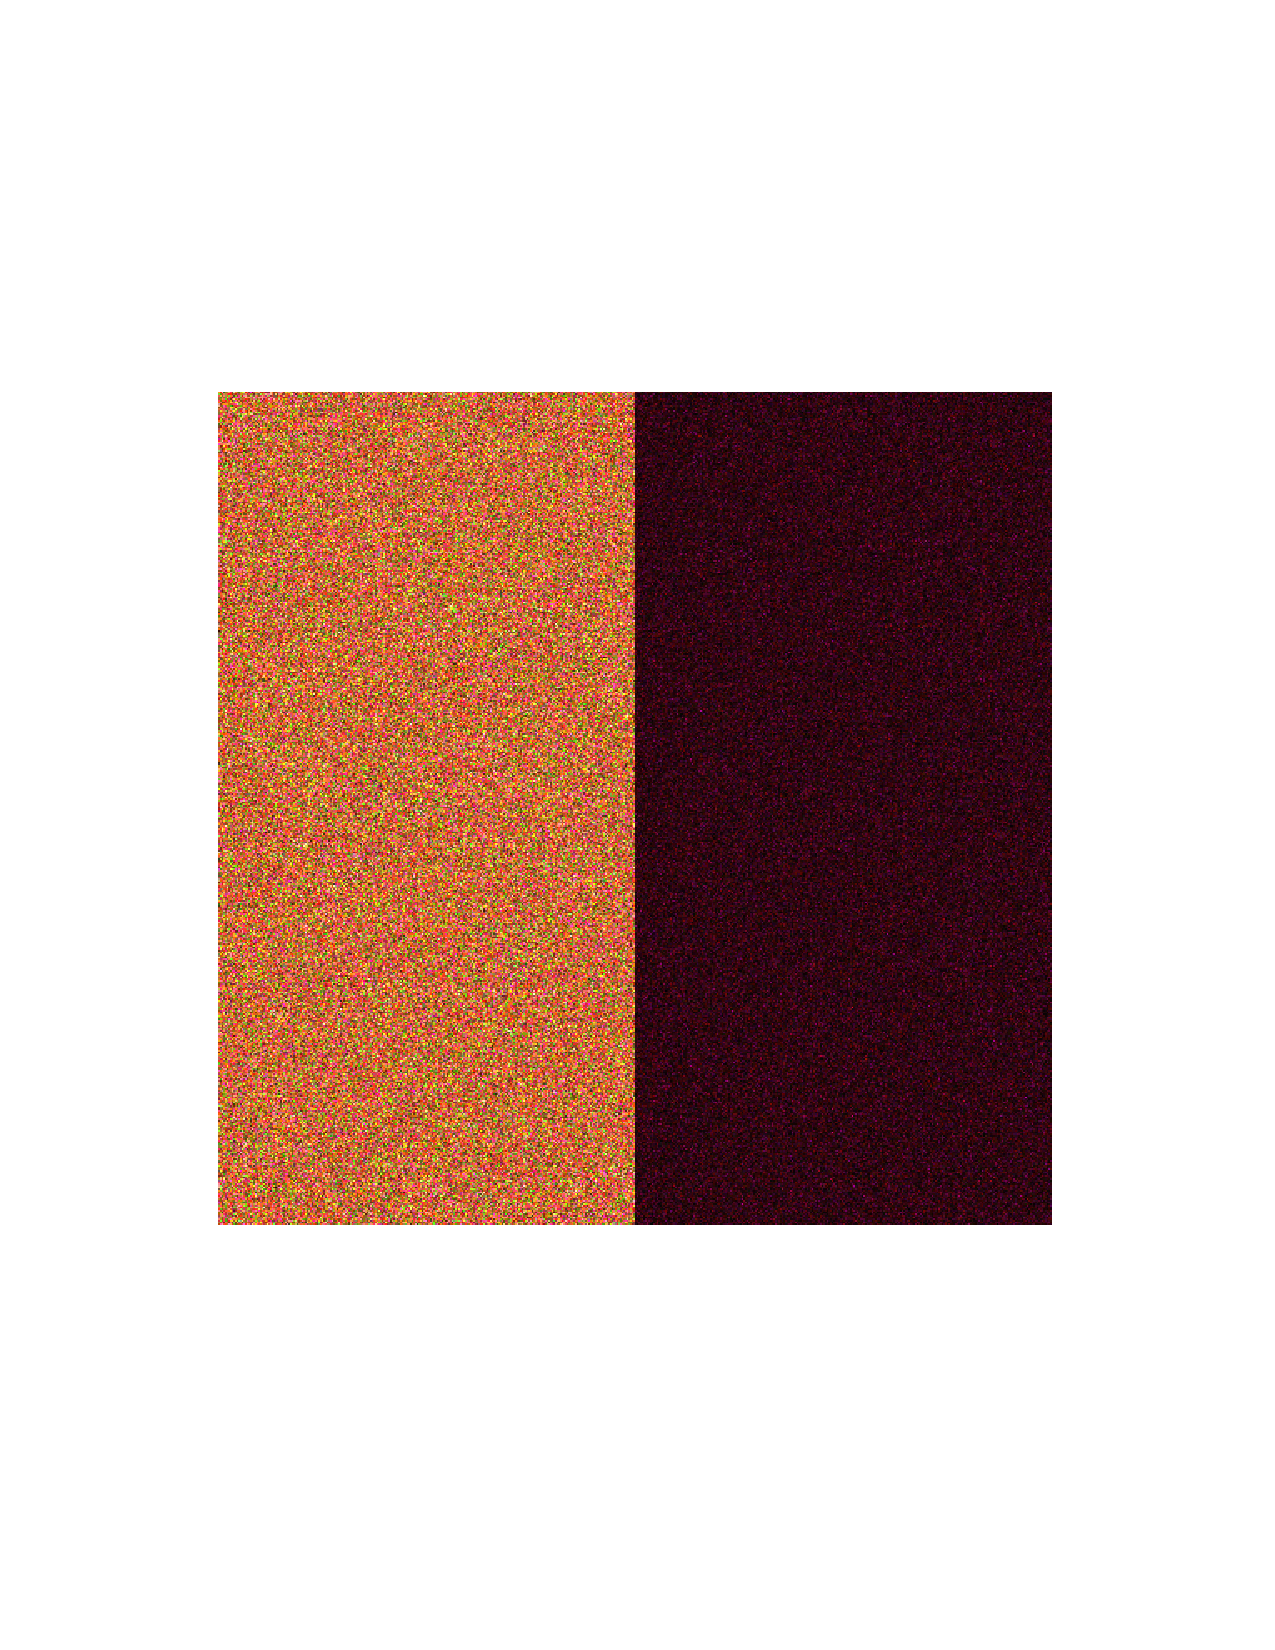
\includegraphics[width=5.0in]{phanton_gamf_dec_pauli.pdf}
	\caption{Decomposição de Pauli uma das phantons com valores de $\Sigma$ propostos no artigo \citep{gamf}.}\label{cap_acf_fig01}
\end{figure}
\begin{figure}[hbt]
	\centering
	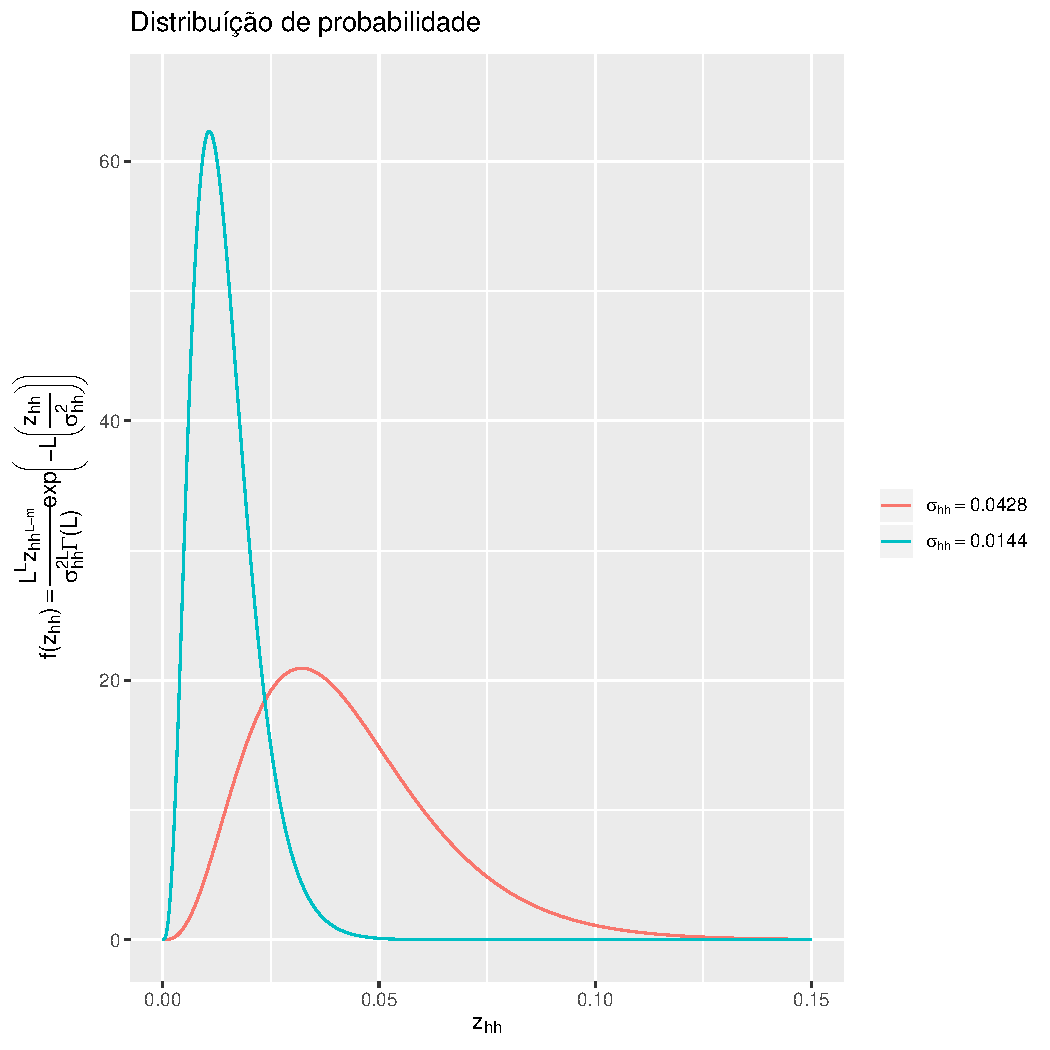
\includegraphics[scale = 0.7]{grafico_pdf_gamf_2017_sigma_hh.pdf}
	\caption{Funções de densidade para dados simulados.}\label{cap_acf_fig02}
\end{figure}

\begin{figure}[hbt]
\minipage{0.5\textwidth}
  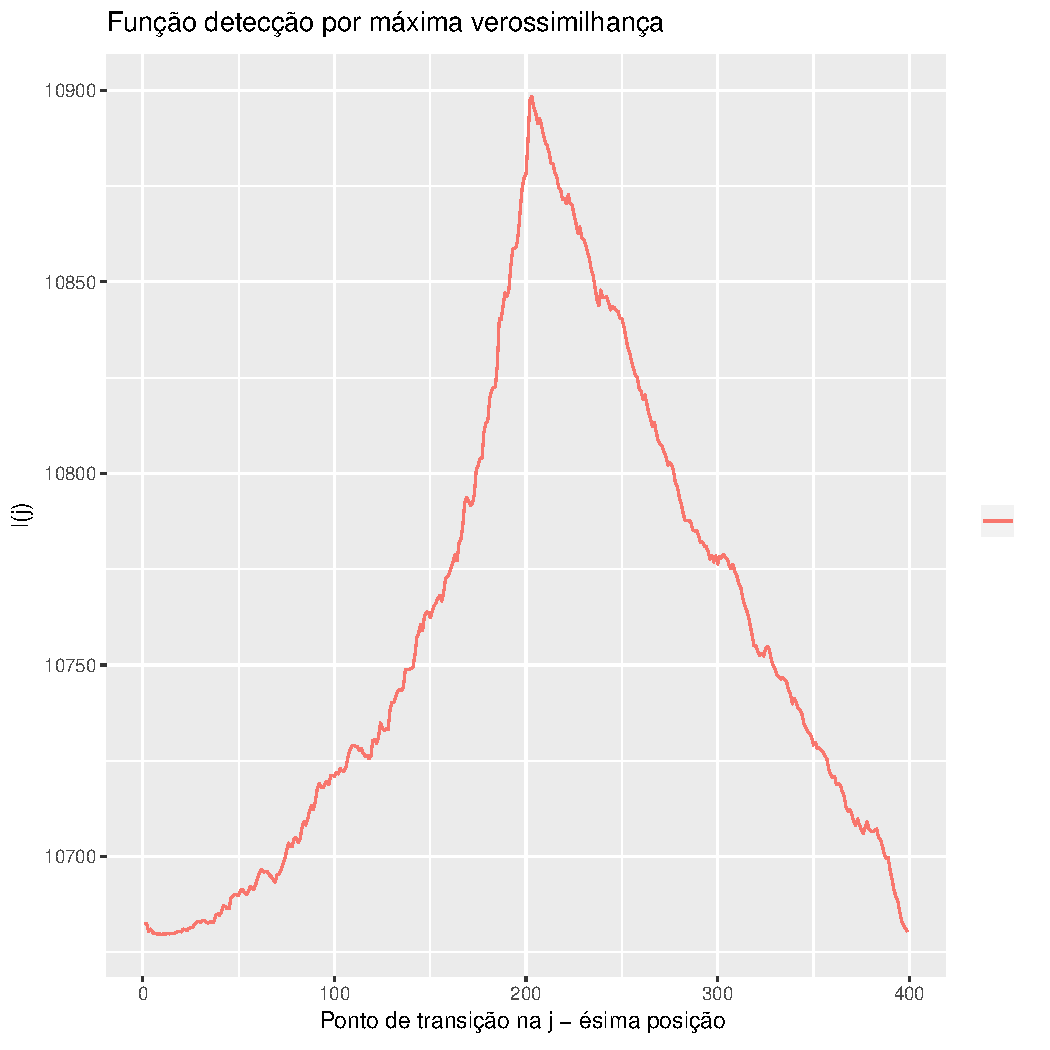
\includegraphics[width=\linewidth]{grafico_l_gamf_2017_sigmahh.pdf}
	\caption{Função $l(j)$ para o canal $I_{HH}$}\label{cap_acf_fig04}
\endminipage\hfill
\minipage{0.5\textwidth}
  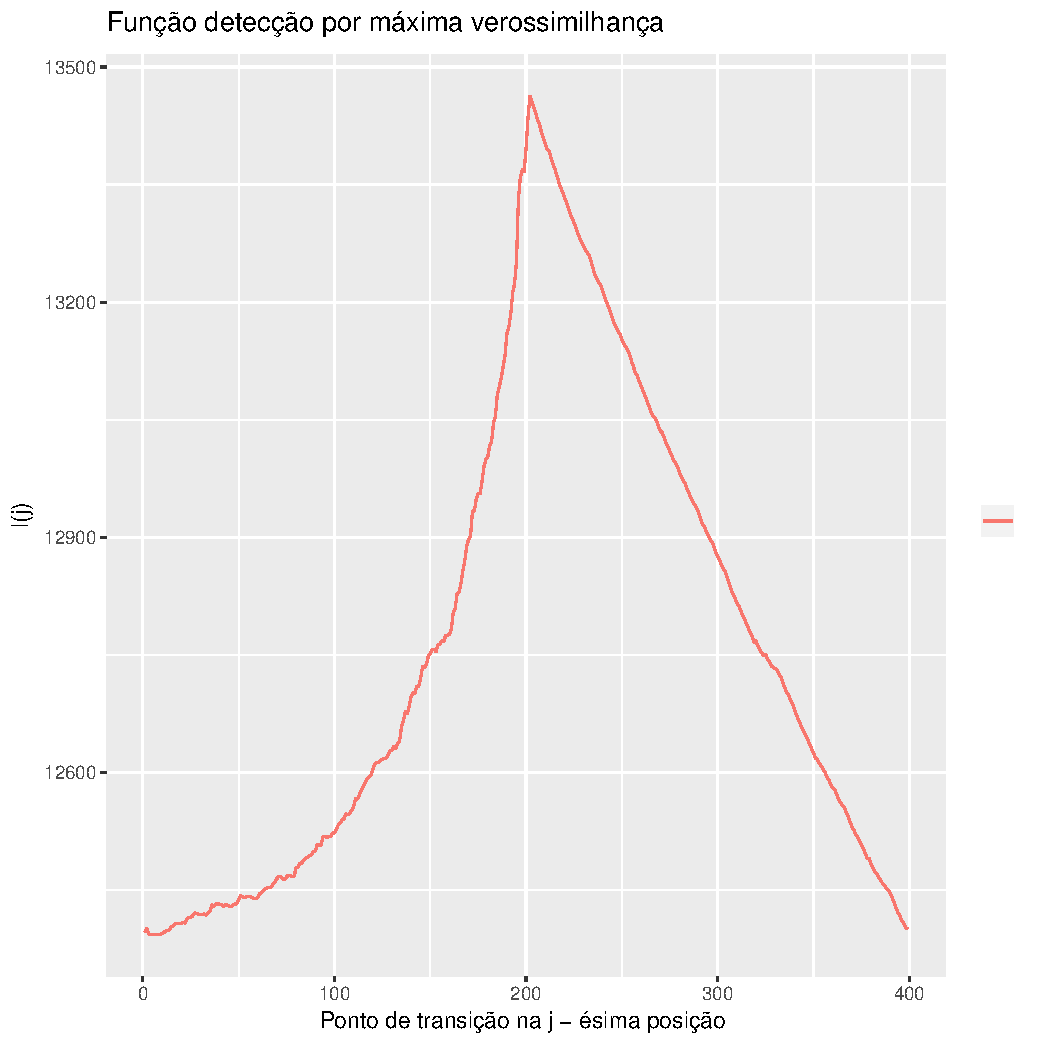
\includegraphics[width=\linewidth]{grafico_l_gamf_2017_sigmahv.pdf}
	\caption{Função $l(j)$ para o canal $I_{HV}$}\label{cap_acf_fig05}
\endminipage\hfill
\centering
\minipage{0.5\textwidth}
  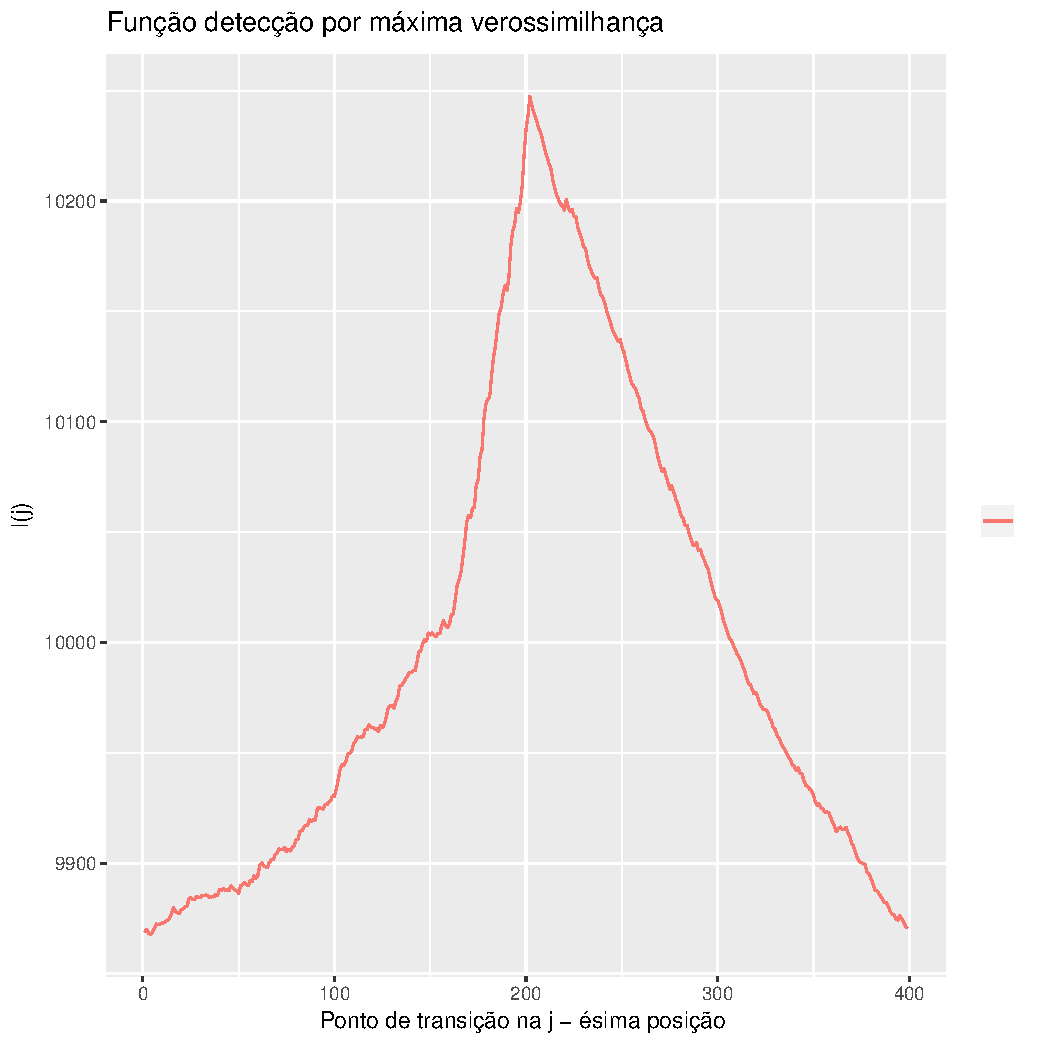
\includegraphics[width=\linewidth]{grafico_l_gamf_2017_sigmavv.pdf}
	\caption{Função $l(j)$ para o canal $I_{VV}$}\label{cap_acf_fig06}
\endminipage\hfill
\end{figure}
\begin{figure}[hbt]
\minipage{0.475\textwidth}
\fbox{  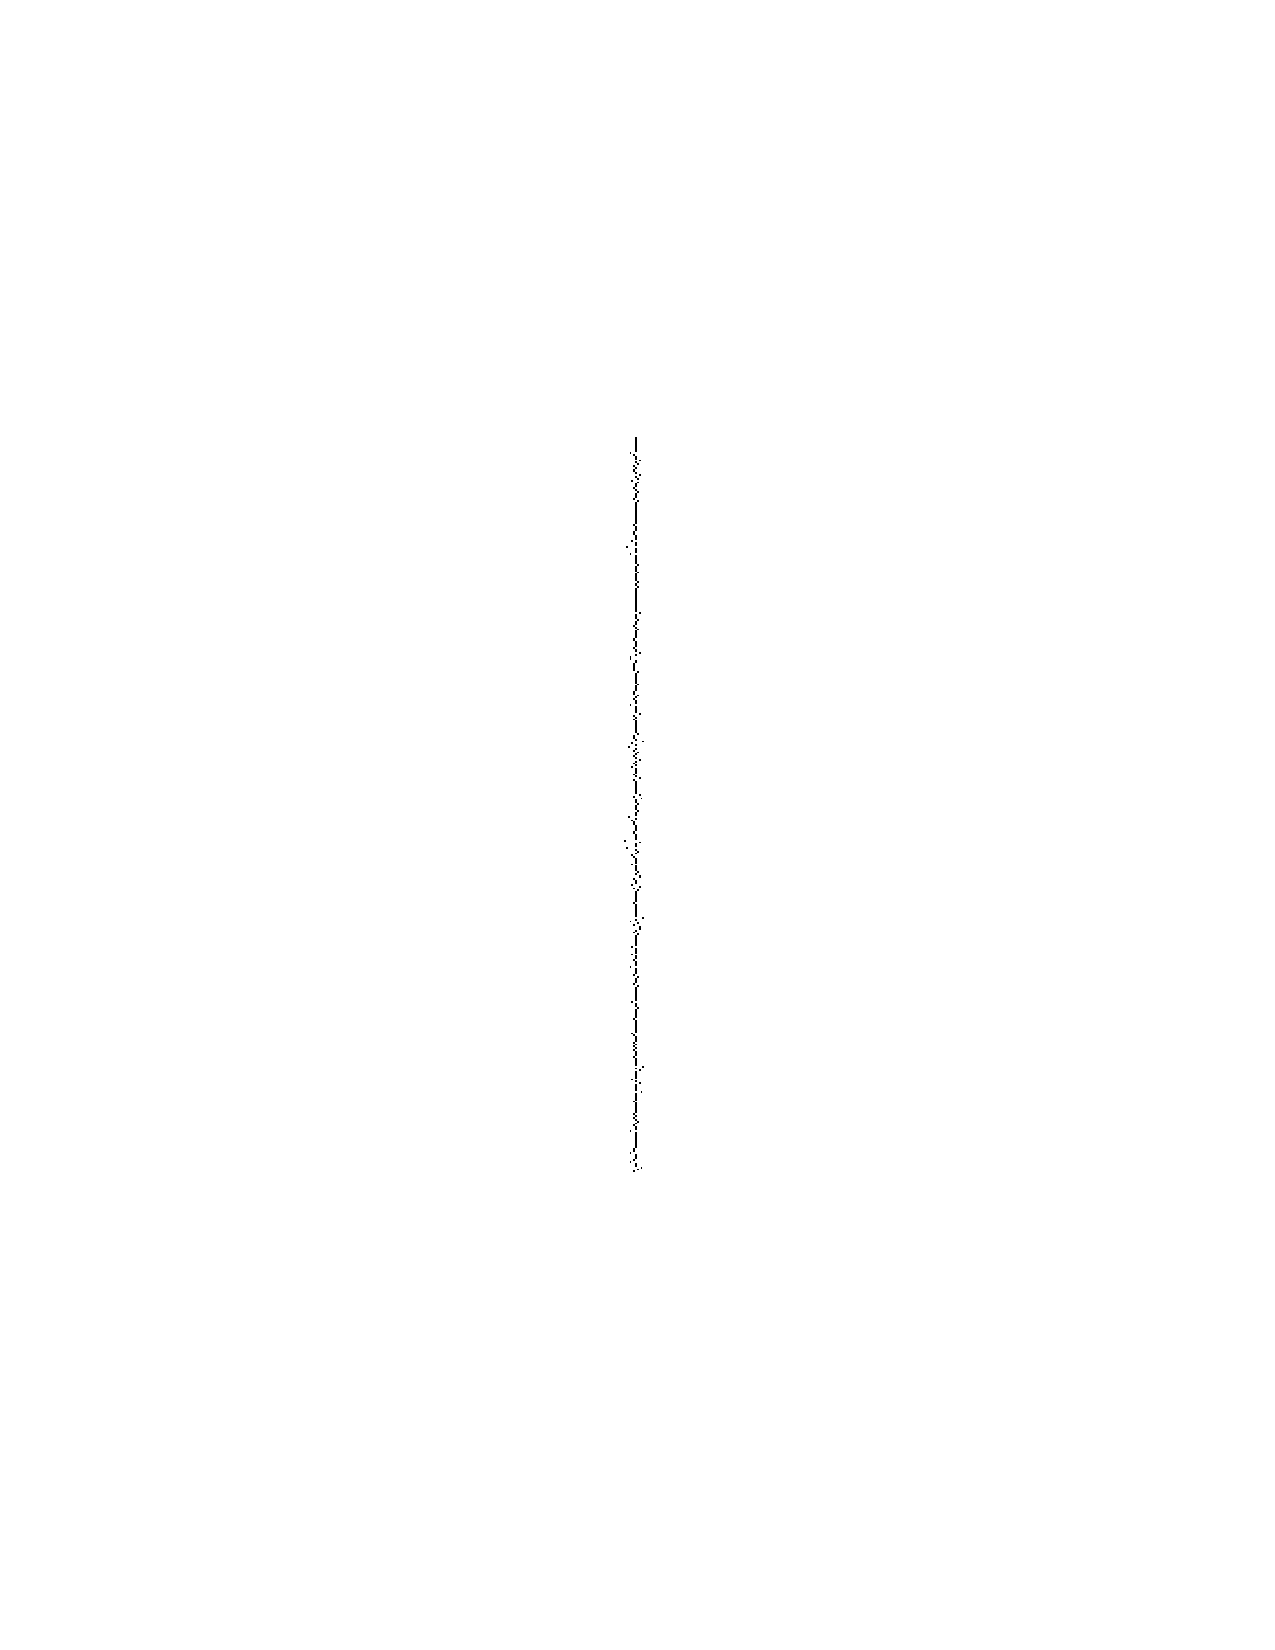
\includegraphics[width=\linewidth]{ev_hh_gamf_2017.pdf}}
\caption{Evidências de bordas para o canal $I_{HH}$}\label{cap_acf_fig07}
\endminipage\hfill
\minipage{0.475\textwidth}
\fbox{ 
\includegraphics[width=\linewidth]{ev_hv_gamf_2017.pdf}}
\caption{Evidências de bordas para o canal $I_{HV}$}\label{cap_acf_fig08}
\endminipage\hfill
\centering
\minipage{0.475\textwidth}
\fbox{ 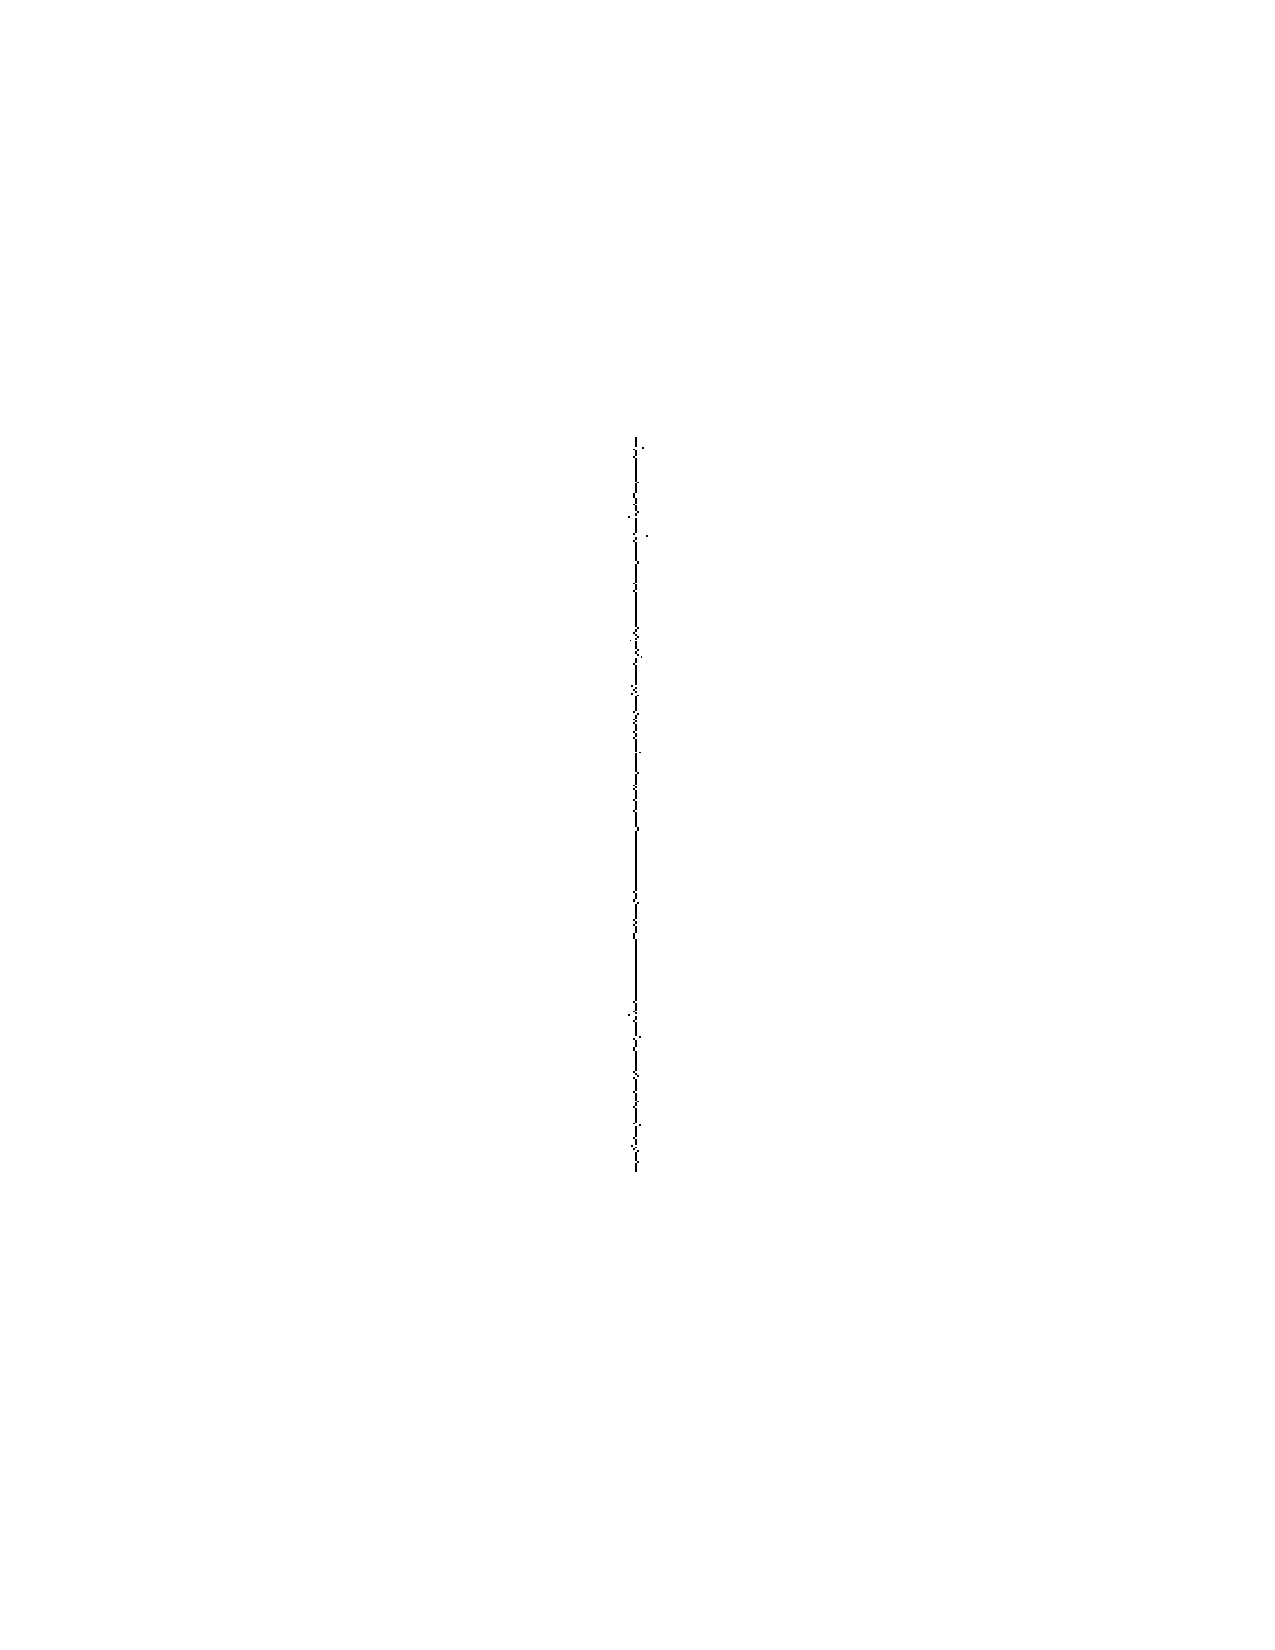
\includegraphics[width=\linewidth]{ev_vv_gamf_2017.pdf}}
\caption{Evidências de bordas para o canal $I_{VV}$}\label{cap_acf_fig09}
\endminipage\hfill
\end{figure}
%
\begin{figure}[hbt]
\centering
	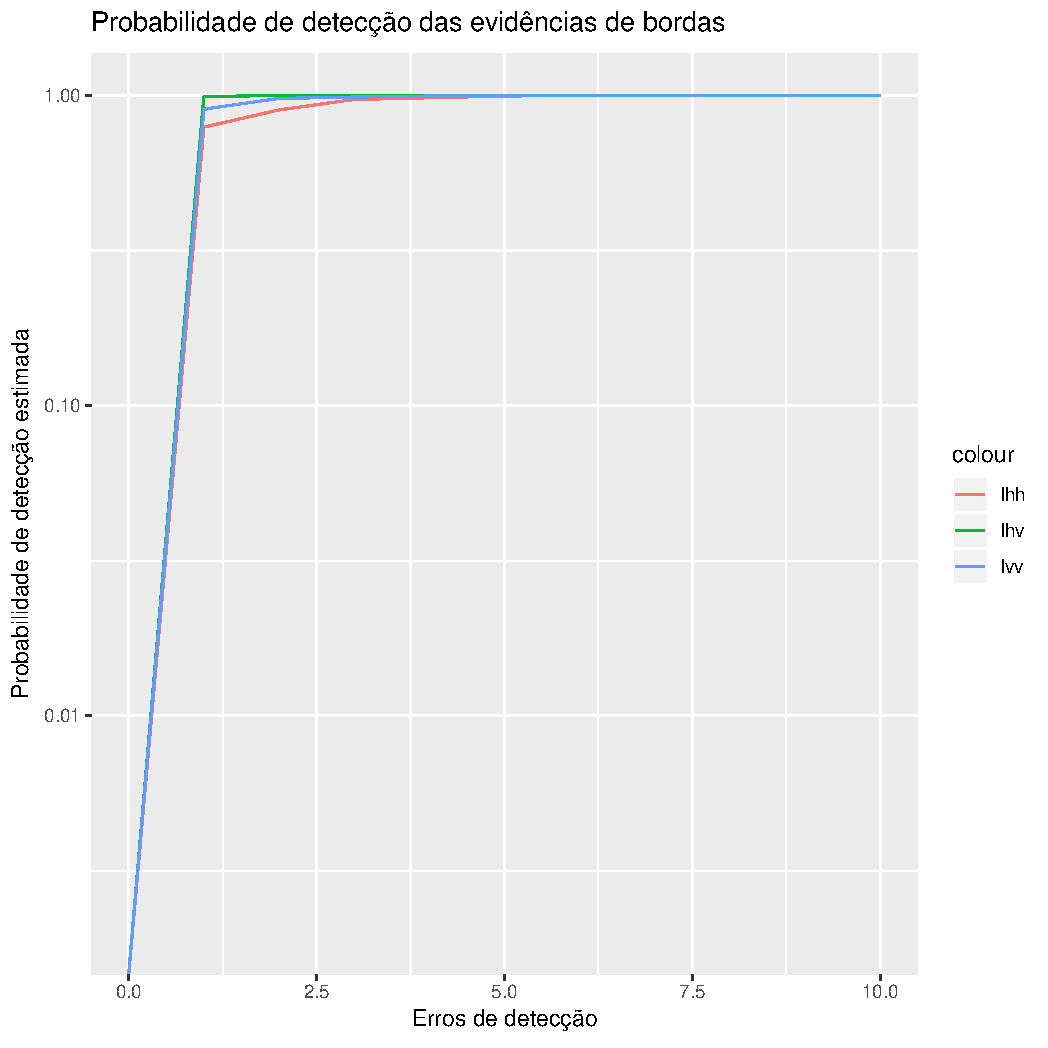
\includegraphics[width=5.0in]{metricas_ihh_ivh_ivv_gamf.pdf}
	\caption{Probabilidade de detecção de borda estimada usando GenSA.}
\label{cap_acf_fig10}
\end{figure}
%
\begin{figure}[hbt]
\minipage{0.475\textwidth}
	\fbox{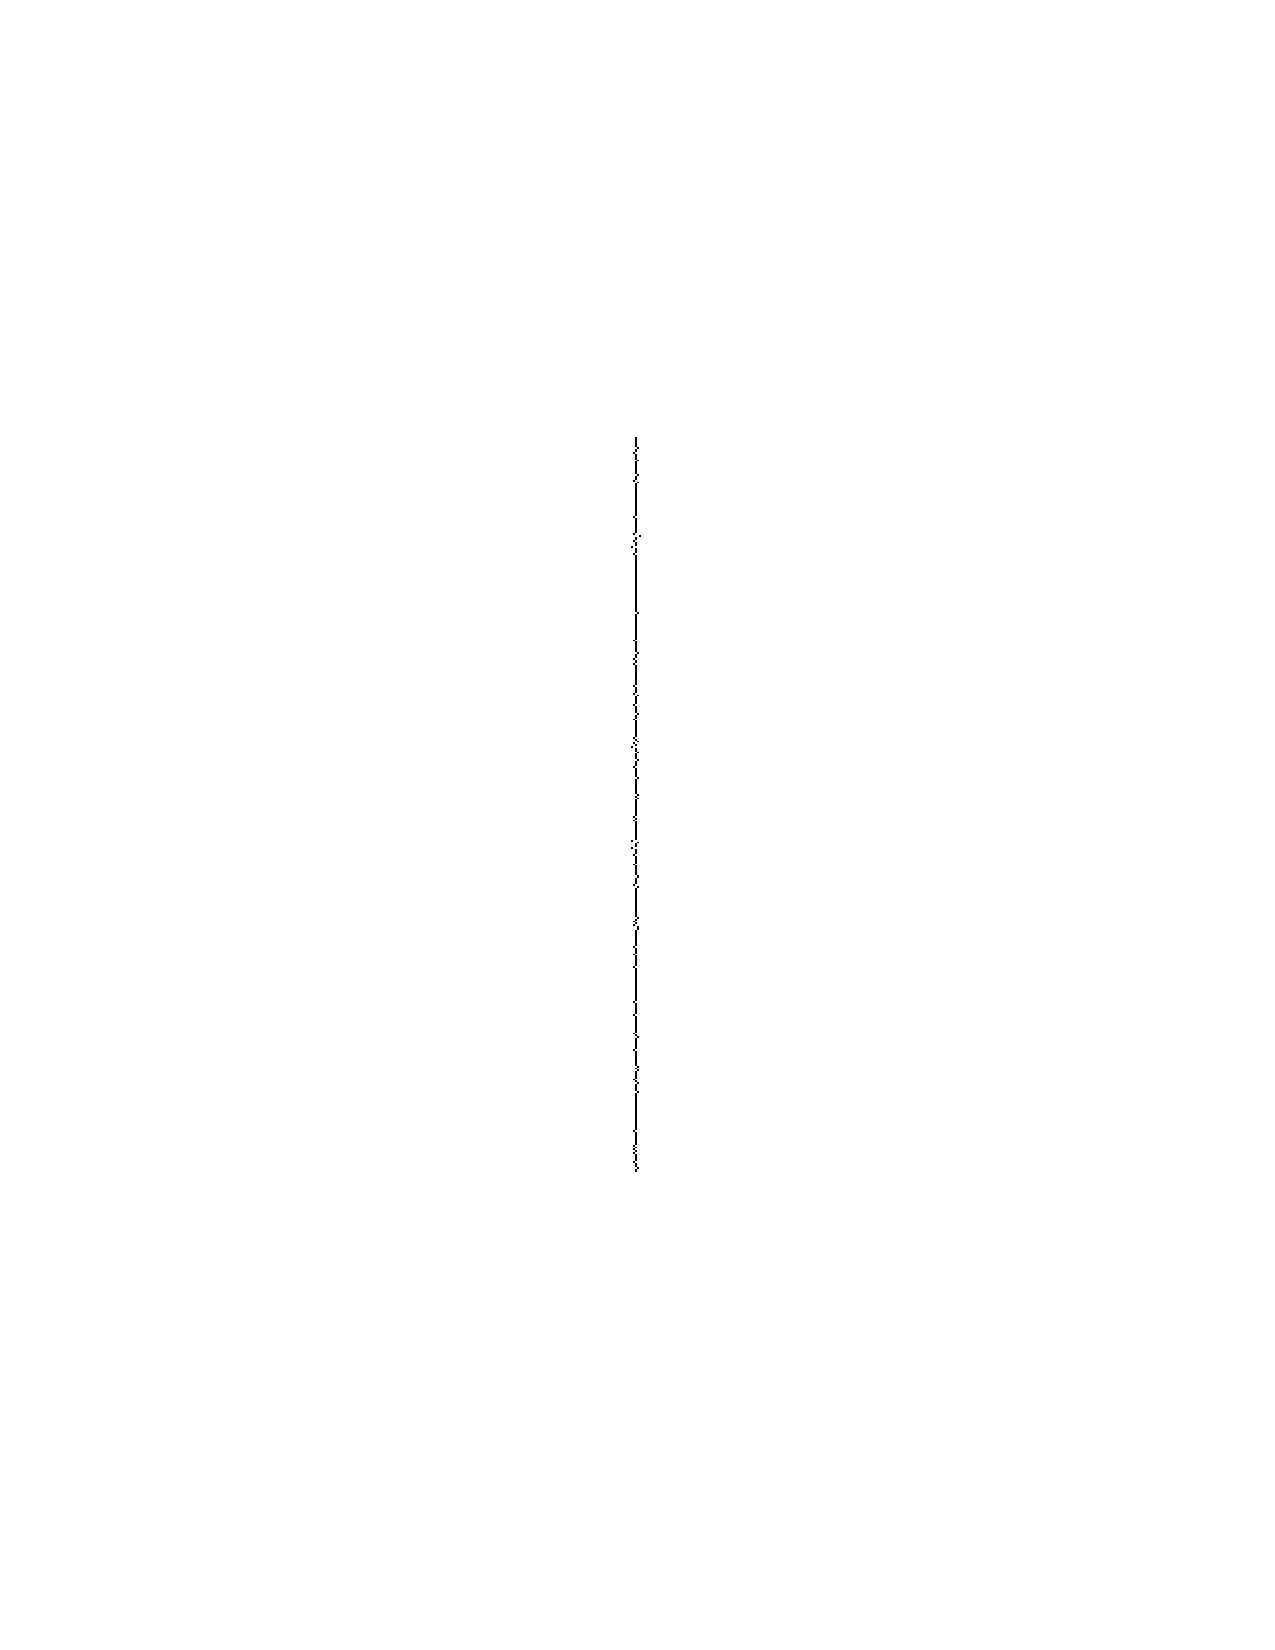
\includegraphics[width=\linewidth]{fusao_soma_ev_hh_hv_vv_gamf.pdf}}
	\caption{Fusão de evidências para os canais $\left(I_{hh}, I_{hv}, I_{vv}\right)$.}
\label{cap_acf_fig11}
\endminipage\hfill
\minipage{0.475\textwidth}
\fbox{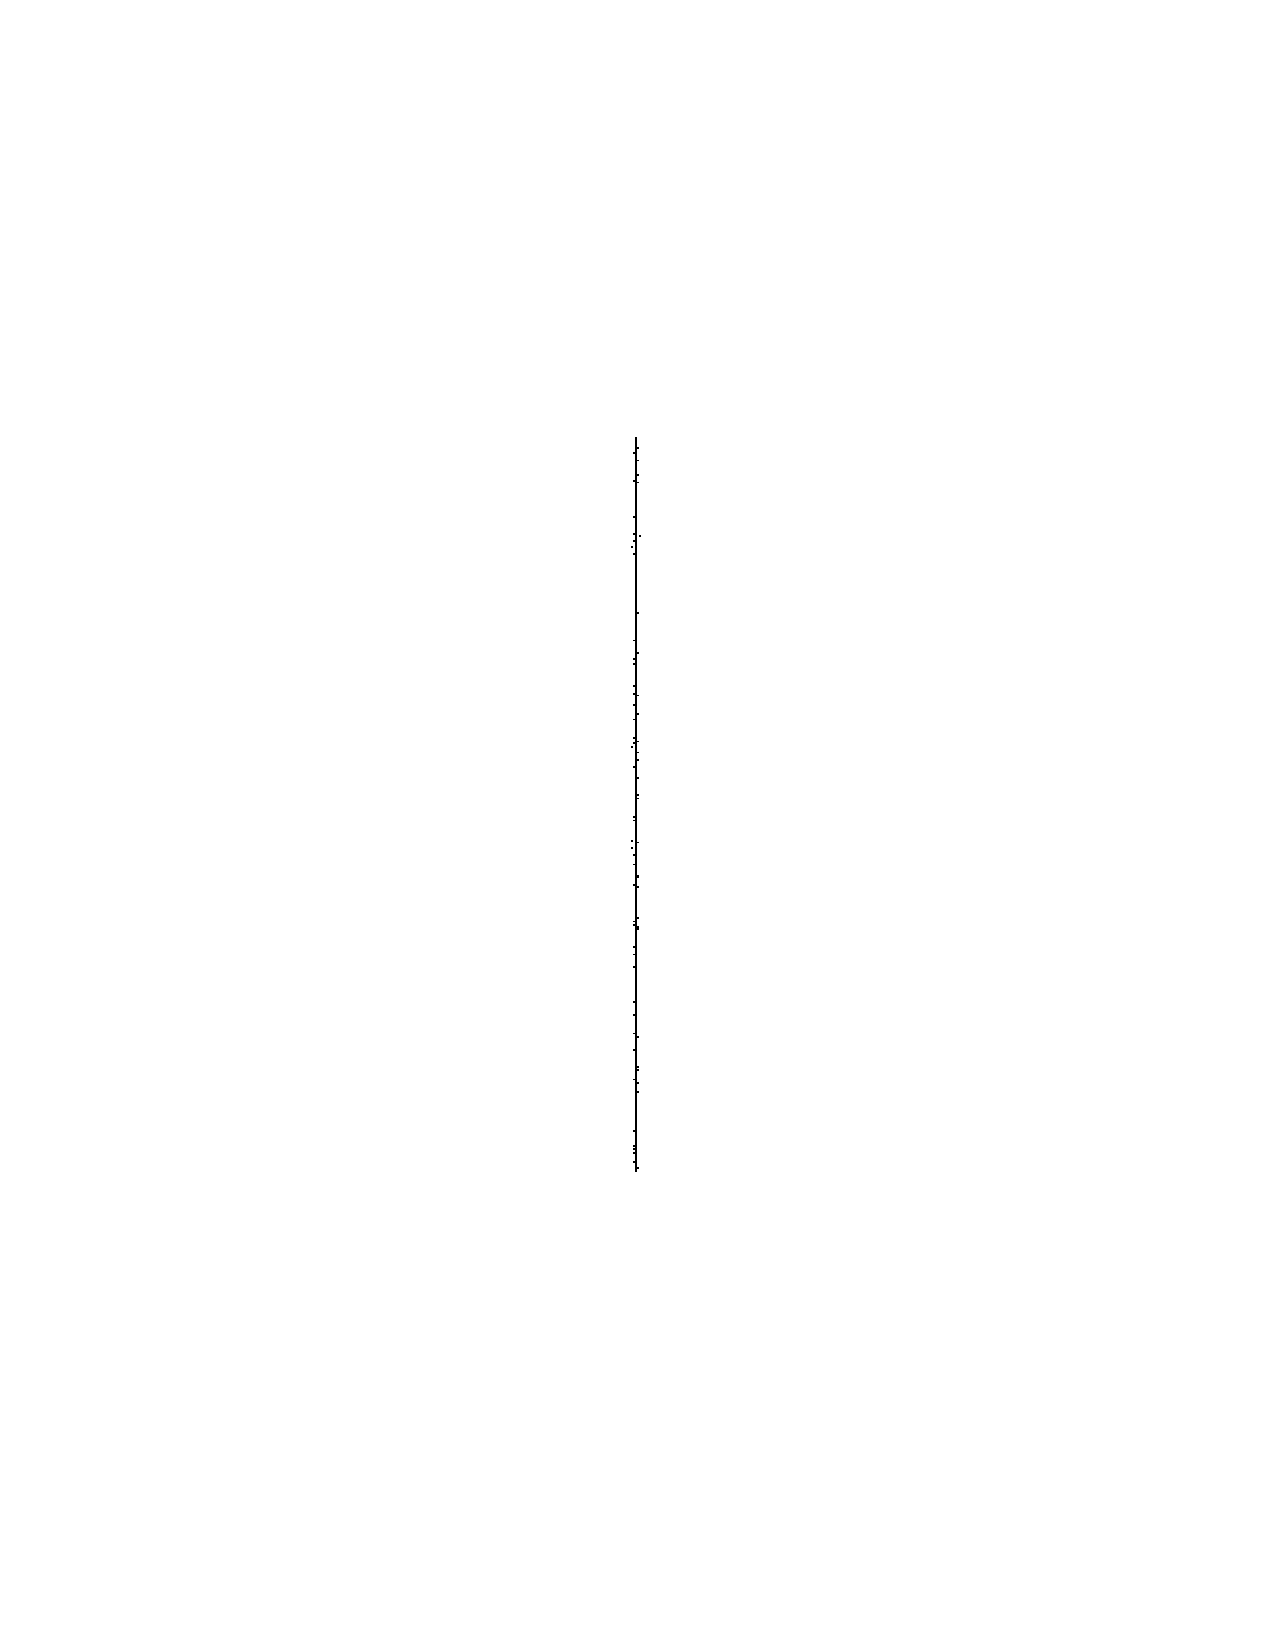
\includegraphics[width=\linewidth]{fusao_ls_gamf.pdf}}	
\caption{Método dos quadrados mínimos aplicado a fusão de imagens.}
\label{cap_acf_fig12}
\endminipage\hfill
\end{figure}
\begin{figure}[hbt]
\minipage{0.475\textwidth}
	\fbox{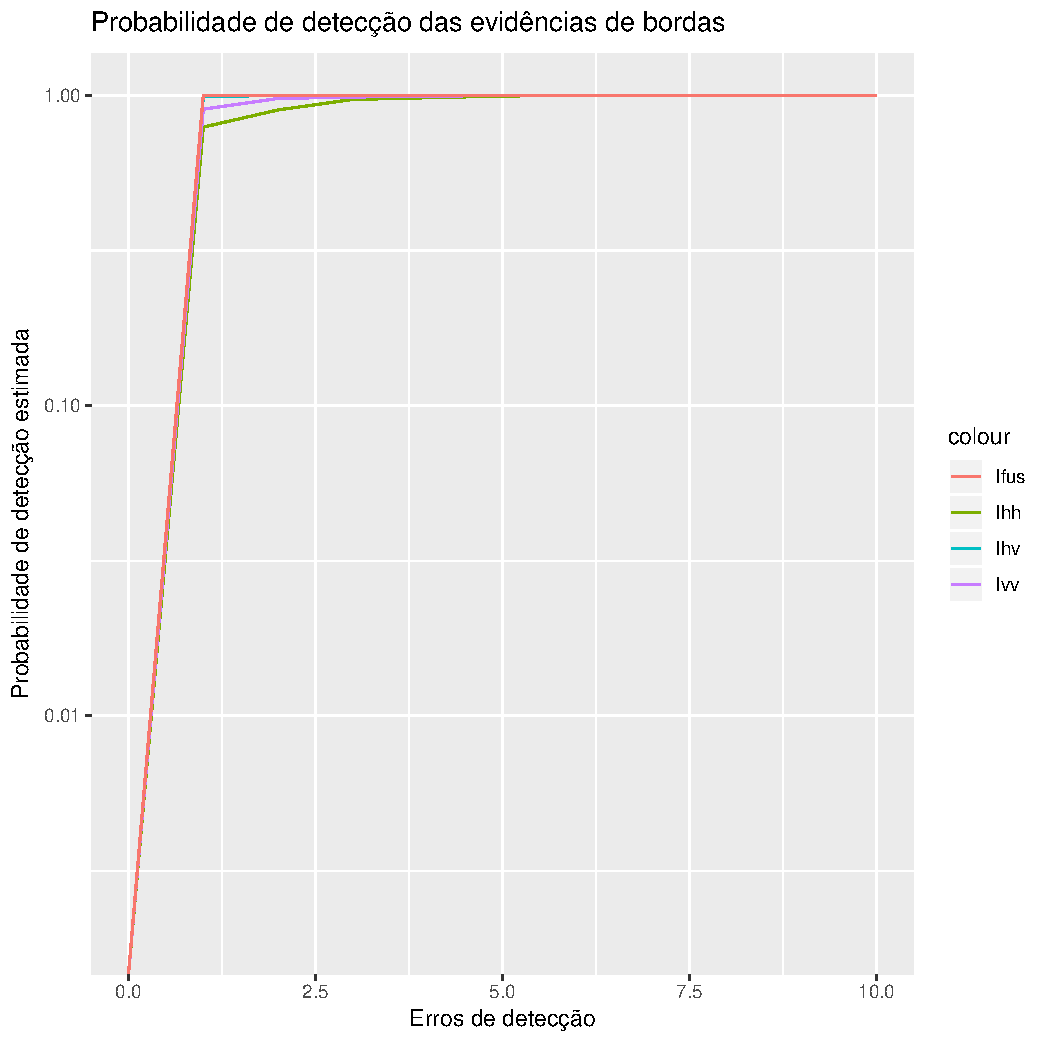
\includegraphics[width=\linewidth]{metricas_ihh_ivh_ivv_ils_gamf.pdf}}
	\caption{Probabilidade de detecção de borda com fusão de evidências.}
\label{cap_acf_fig13}
\endminipage\hfill
\minipage{0.475\textwidth}
\fbox{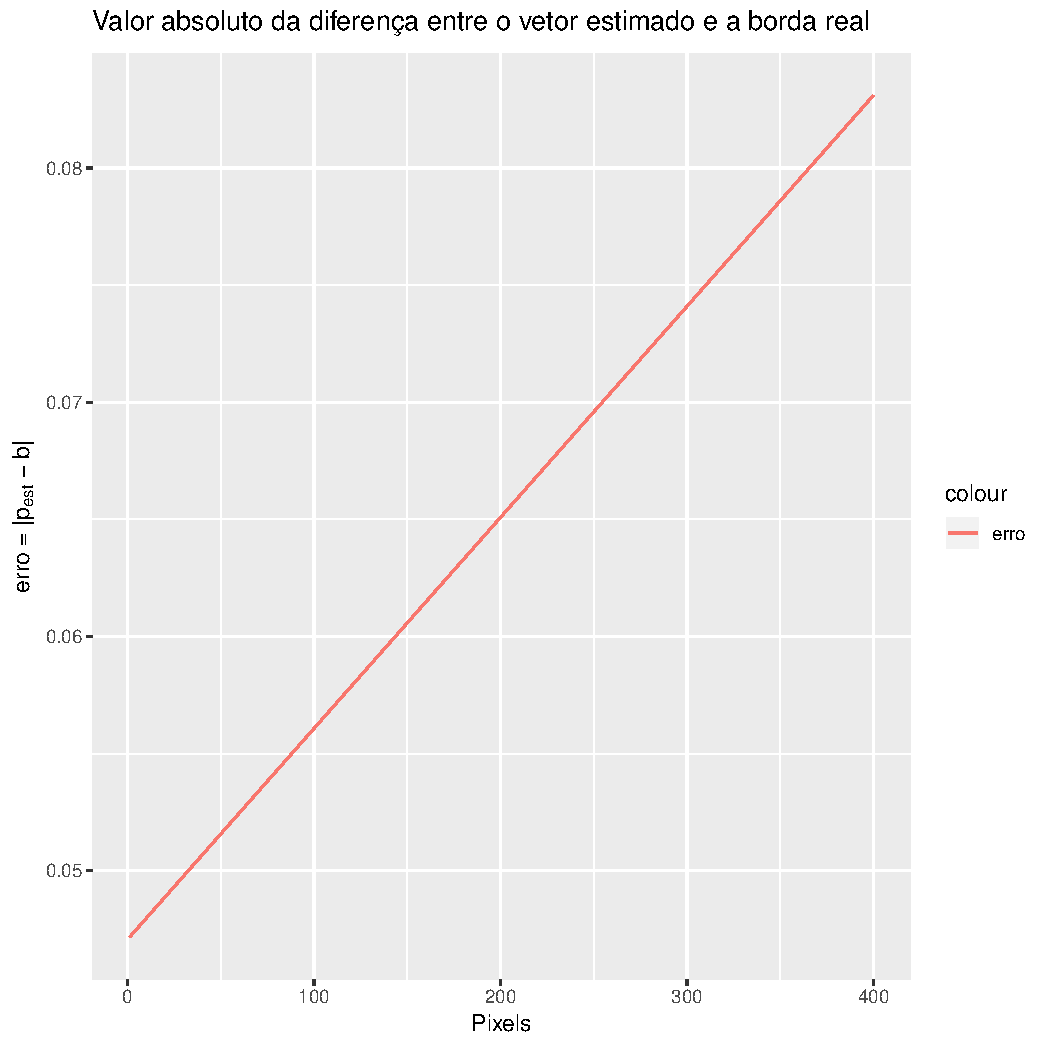
\includegraphics[width=\linewidth]{fusao_ls_erro_gamf.pdf}}	
	\caption{Valor absoluto da diferença entre o vetor estimado da fusão de evidências e a borda real.}
\label{cap_acf_fig14}
\endminipage\hfill
\end{figure}
\section{Sigmas do artigo}
\begin{figure}[hbt]
\centering
	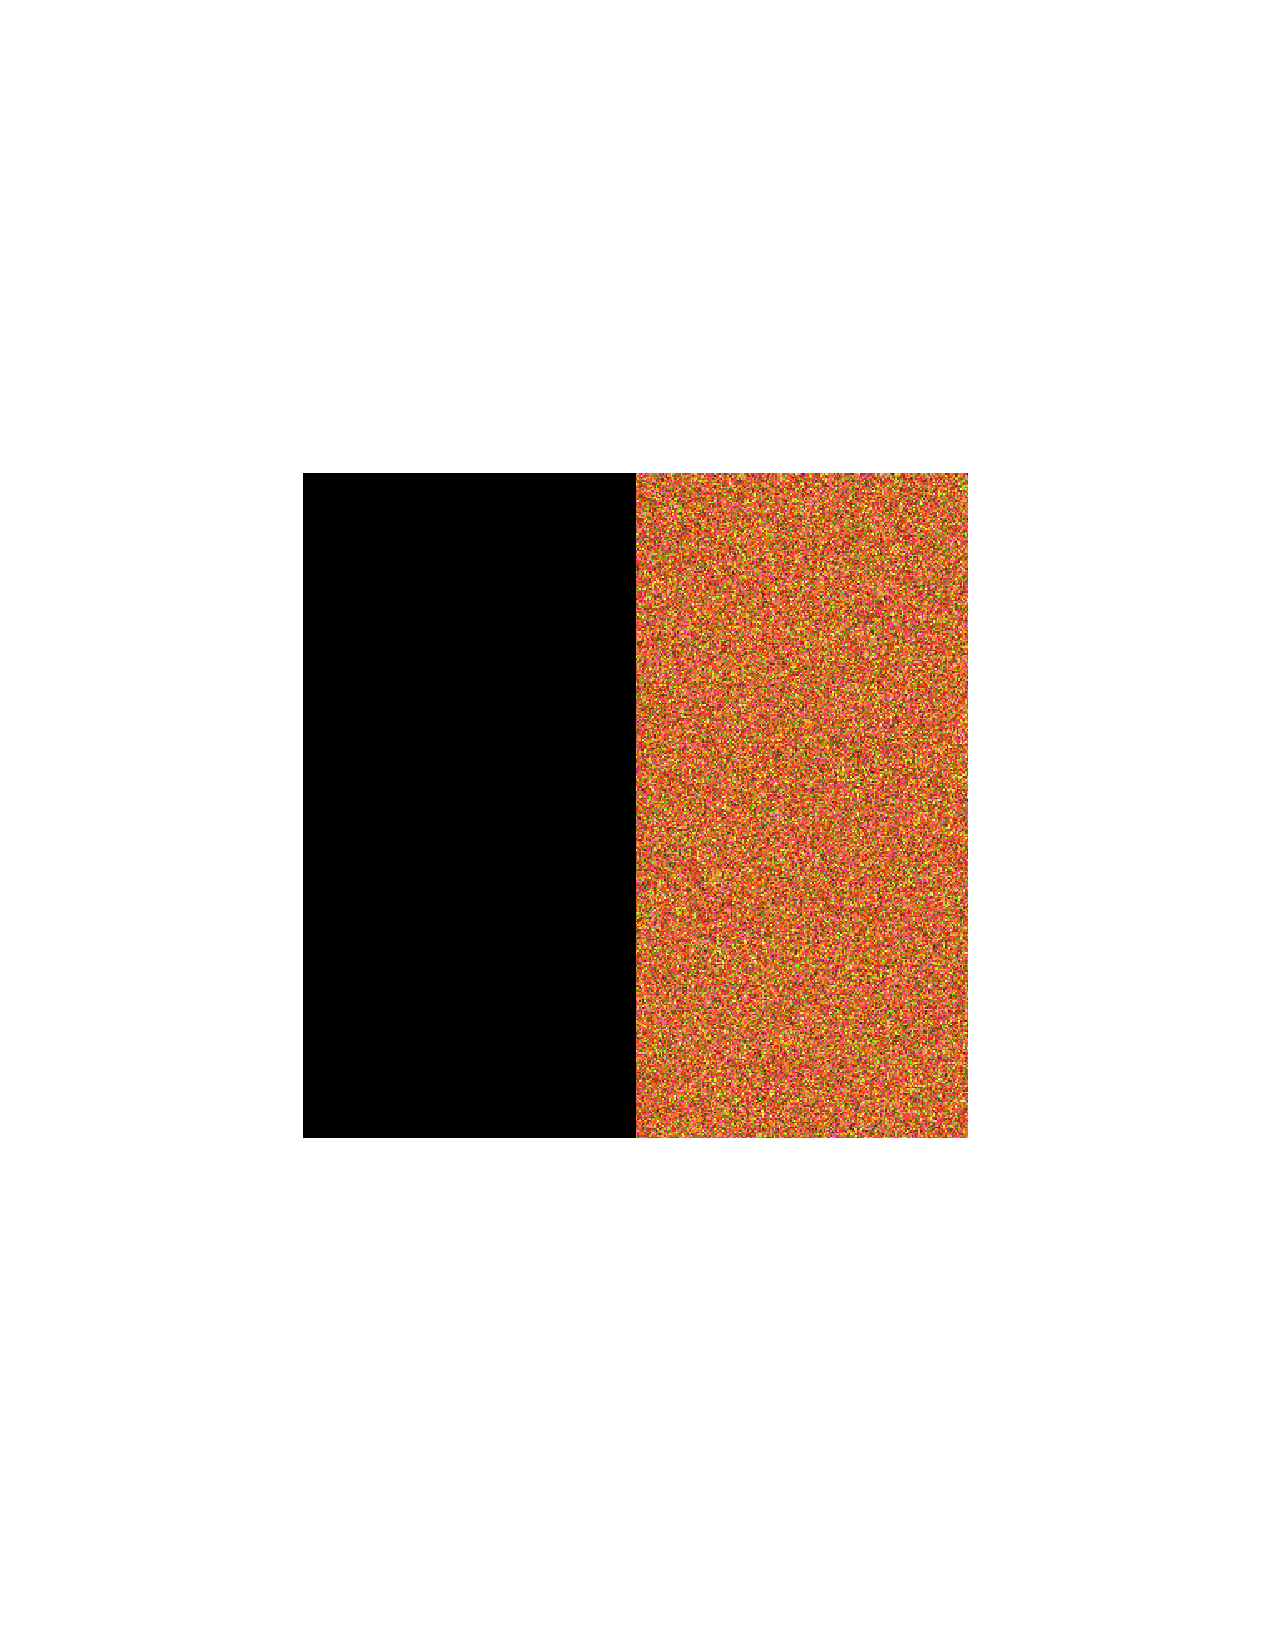
\includegraphics[width=5.0in]{phanton_vert_dec_pauli.pdf}
	\caption{Decomposição de Pauli uma das phantons com valores de $\Sigma$ propostos no artigo \citep{gamf}.}\label{cap_acf_fig01}
\end{figure}
\begin{figure}[hbt]
\minipage{0.5\textwidth}
  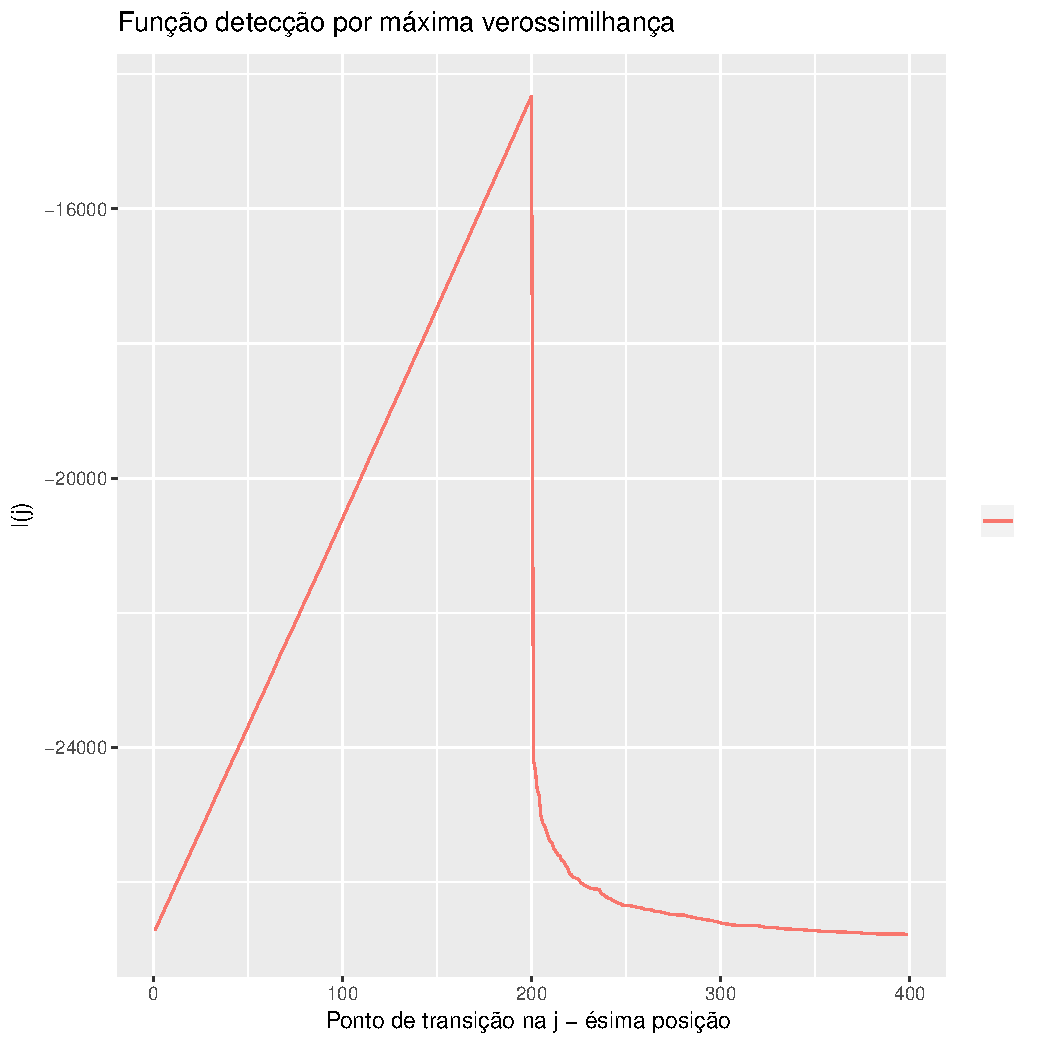
\includegraphics[width=\linewidth]{grafico_l_vert_sigmahh.pdf}
	\caption{Função $l(j)$ para o canal $I_{HH}$}\label{cap_acf_fig04}
\endminipage\hfill
\minipage{0.5\textwidth}
  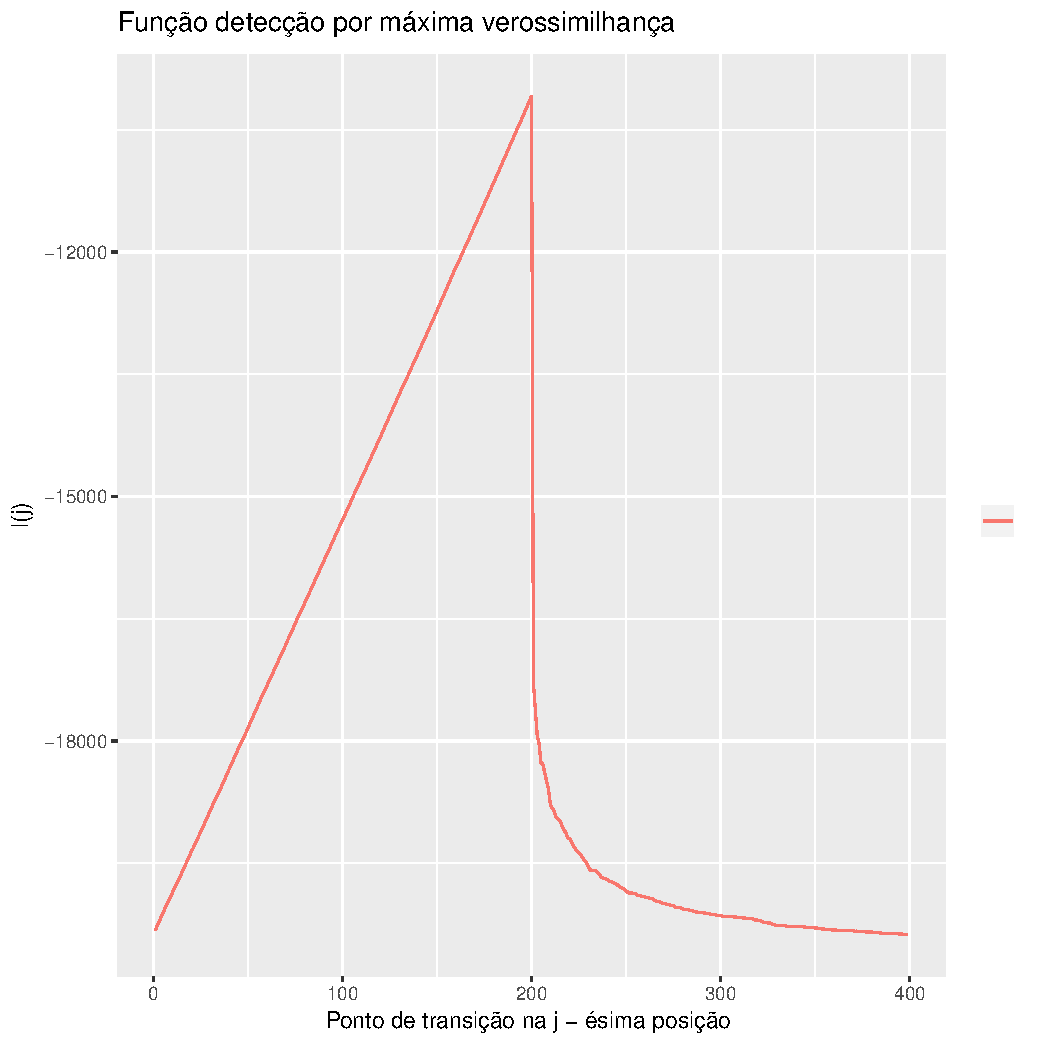
\includegraphics[width=\linewidth]{grafico_l_vert_sigmahv.pdf}
	\caption{Função $l(j)$ para o canal $I_{HV}$}\label{cap_acf_fig05}
\endminipage\hfill
\centering
\minipage{0.5\textwidth}
  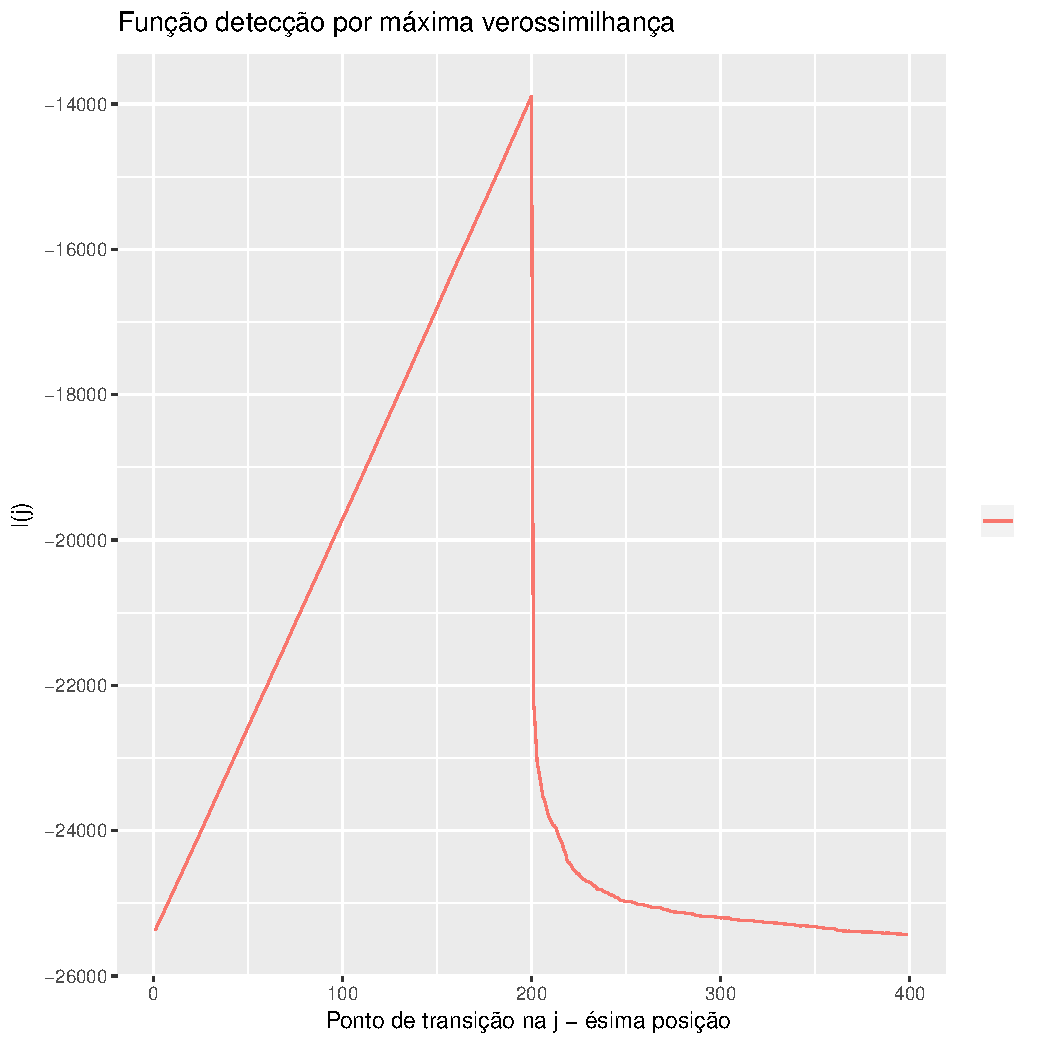
\includegraphics[width=\linewidth]{grafico_l_vert_sigmavv.pdf}
	\caption{Função $l(j)$ para o canal $I_{VV}$}\label{cap_acf_fig06}
\endminipage\hfill
\end{figure}
\begin{figure}[hbt]
\minipage{0.475\textwidth}
\fbox{  
\includegraphics[width=\linewidth]{ev_hh_vert.pdf}}
\caption{Evidências de bordas para o canal $I_{HH}$}\label{cap_acf_fig07}
\endminipage\hfill
\minipage{0.475\textwidth}
\fbox{ 
\includegraphics[width=\linewidth]{ev_hv_vert.pdf}}
\caption{Evidências de bordas para o canal $I_{HV}$}\label{cap_acf_fig08}
\endminipage\hfill
\centering
\minipage{0.475\textwidth}
\fbox{ 
\includegraphics[width=\linewidth]{ev_vv_vert.pdf}}
\caption{Evidências de bordas para o canal $I_{VV}$}\label{cap_acf_fig09}
\endminipage\hfill
\end{figure}
\begin{figure}[hbt]
\centering
	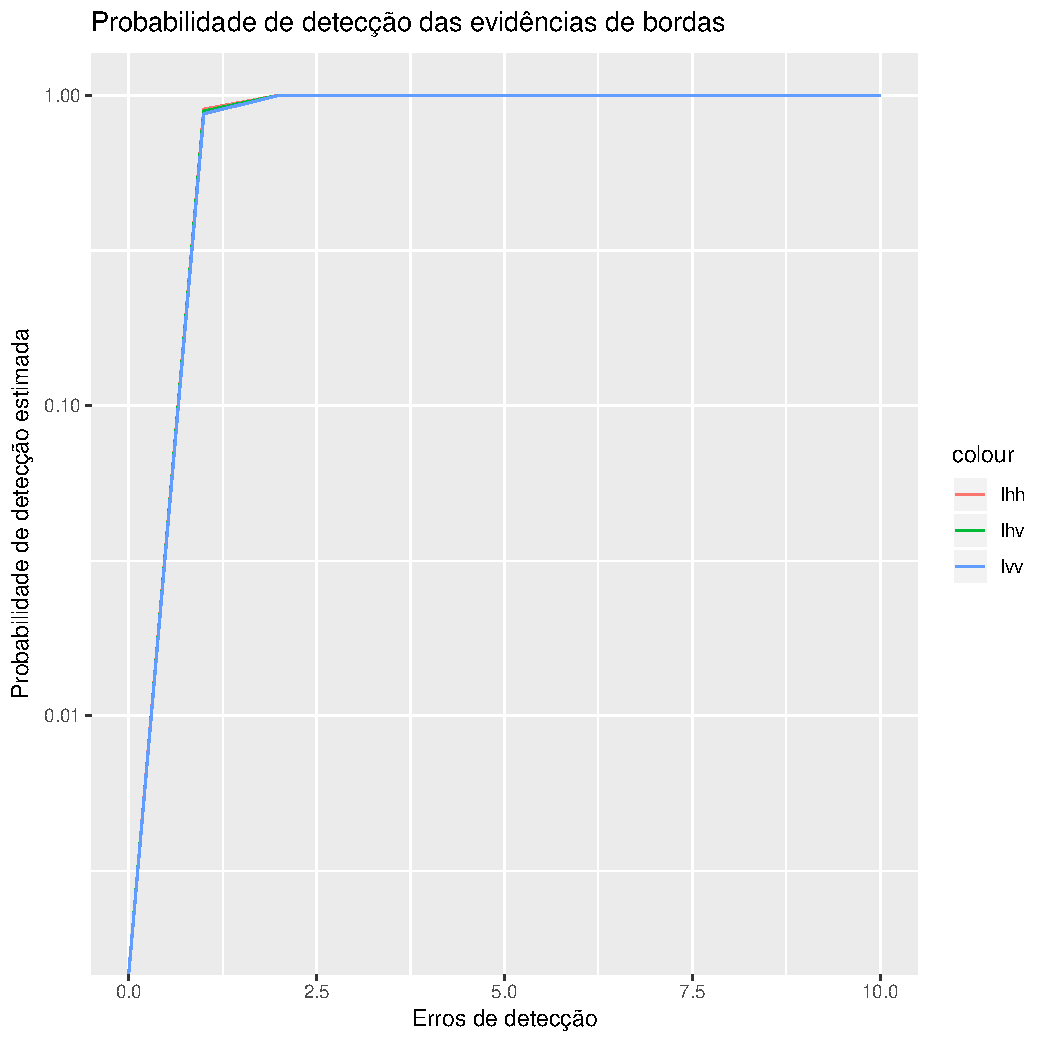
\includegraphics[width=5.0in]{metricas_ihh_ivh_ivv_vert.pdf}
	\caption{Probabilidade de detecção de borda estimada usando GenSA.}
\label{cap_acf_fig10}
\end{figure}
%
\begin{figure}[hbt]
\minipage{0.475\textwidth}
	\fbox{
\includegraphics[width=\linewidth]{fusao_soma_ev_hh_hv_vv_vert.pdf}}
	\caption{Fusão de evidências para os canais $\left(I_{hh}, I_{hv}, I_{vv}\right)$.}
\label{cap_acf_fig11}
\endminipage\hfill
\minipage{0.475\textwidth}
\fbox{
\includegraphics[width=\linewidth]{fusao_ls_vert.pdf}}	
\caption{Método dos quadrados mínimos aplicado a fusão de imagens.}
\label{cap_acf_fig12}
\endminipage\hfill
\end{figure}
\begin{figure}[hbt]
\minipage{0.475\textwidth}
	\fbox{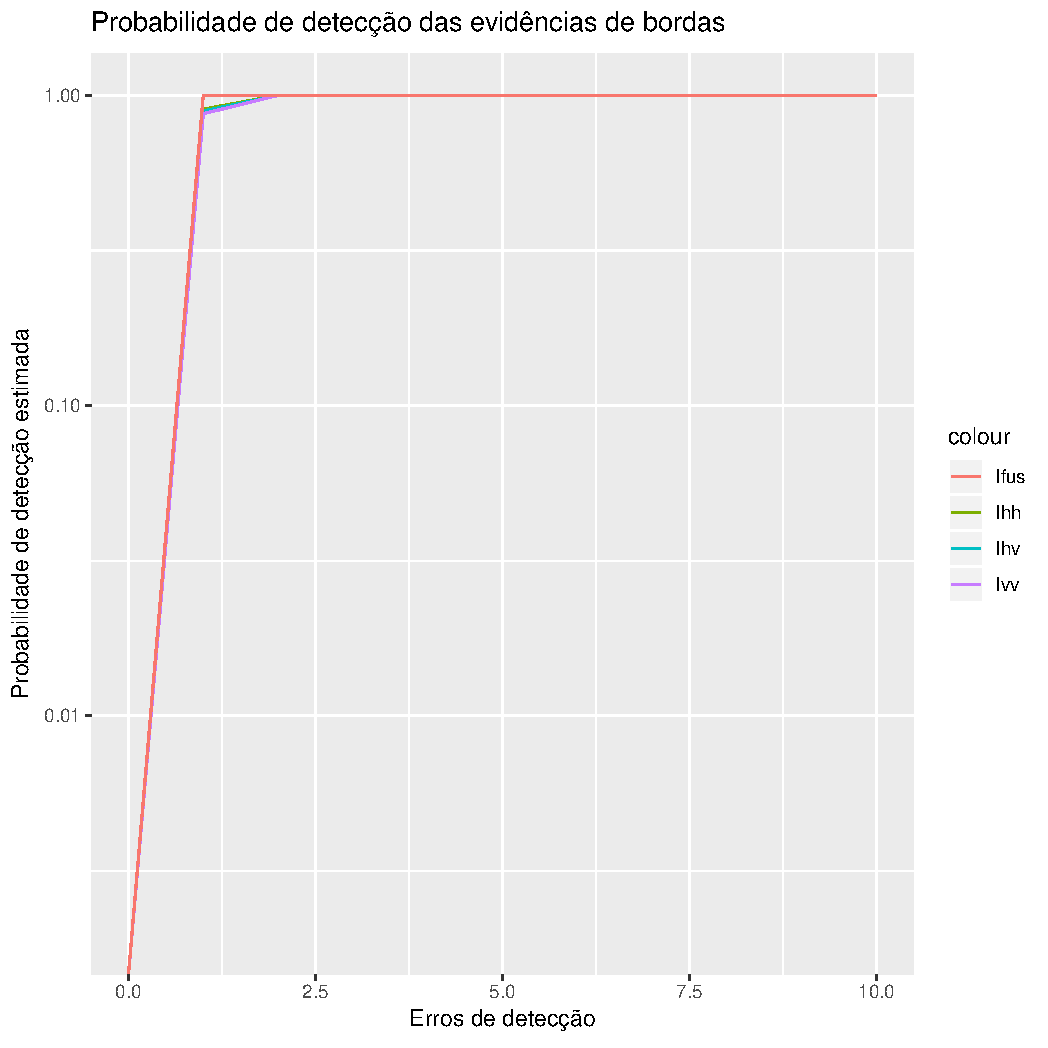
\includegraphics[width=\linewidth]{metricas_ihh_ivh_ivv_ils_vert.pdf}}
	\caption{Probabilidade de detecção de borda com fusão de evidências.}
\label{cap_acf_fig13}
\endminipage\hfill
\minipage{0.475\textwidth}
\fbox{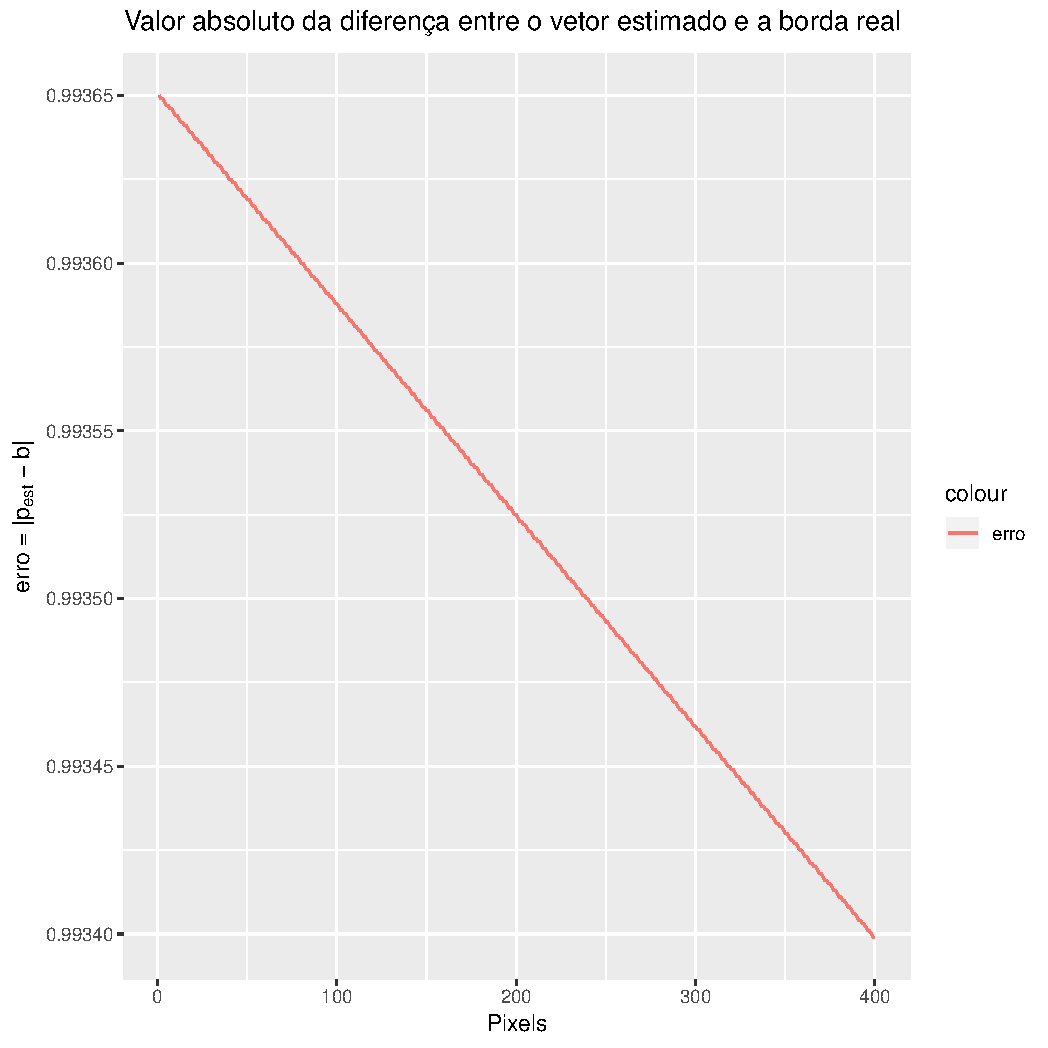
\includegraphics[width=\linewidth]{fusao_ls_erro_vert.pdf}}	
	\caption{Valor absoluto da diferença entre o vetor estimado da fusão de evidências e a borda real.}
\label{cap_acf_fig14}
\endminipage\hfill
\end{figure}
Sigmas da referência \citet{nhfc}.
\begin{figure}[hbt]
\minipage{0.475\textwidth}
	\fbox{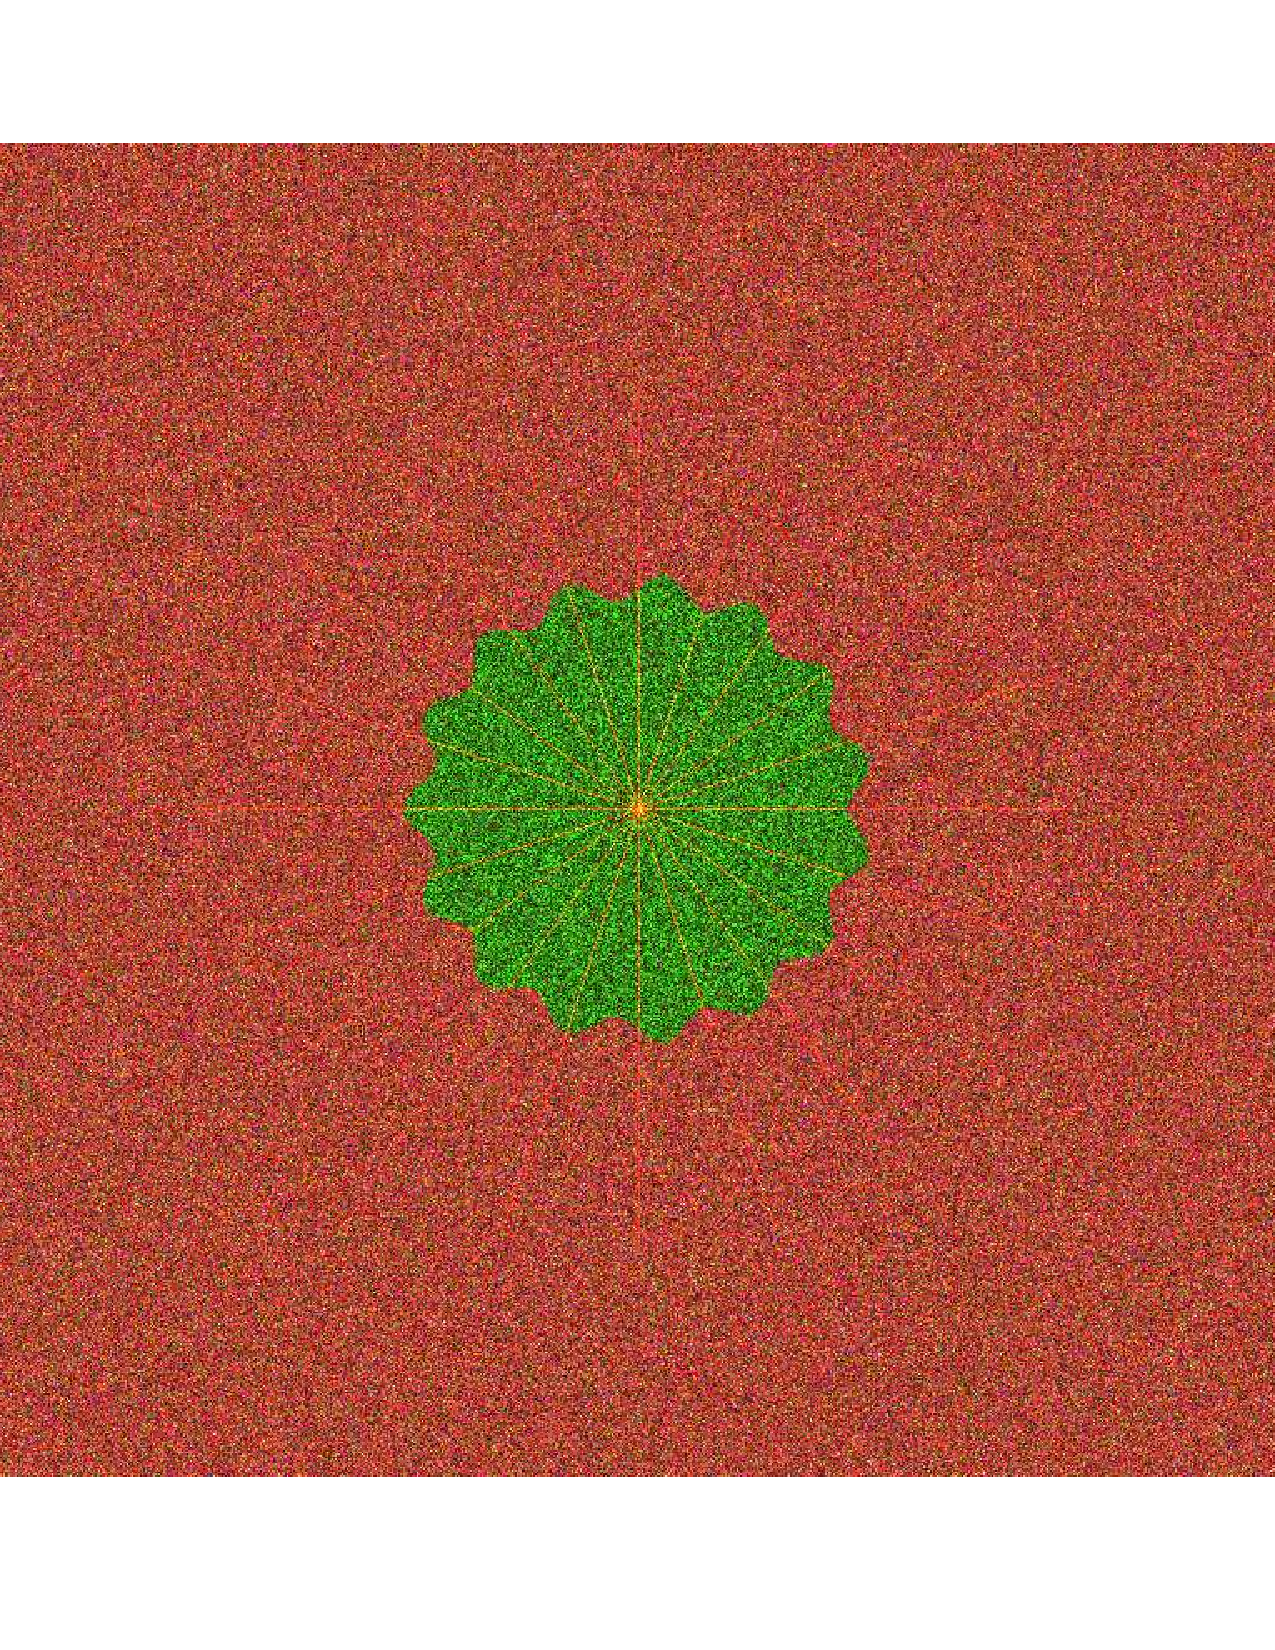
\includegraphics[width=\linewidth]{flor_15_133_8_pauli.pdf}}
	\caption{Imagem flor simulada com $\beta = 15$, $\delta = 133$ e $\nu = 8$ .}
\label{cap_acf_fig15}
\endminipage\hfill
\minipage{0.475\textwidth}
\fbox{
\includegraphics[width=\linewidth]{flor_15_133_8_bin.pdf}}	
	\caption{Imagem flor simulada binária com $\beta = 15$, $\delta = 133$ e $\nu = 8$ .}
\label{cap_acf_fig16}
\endminipage\hfill
\end{figure}
\begin{figure}[hbt]
\minipage{0.475\textwidth}
\fbox{  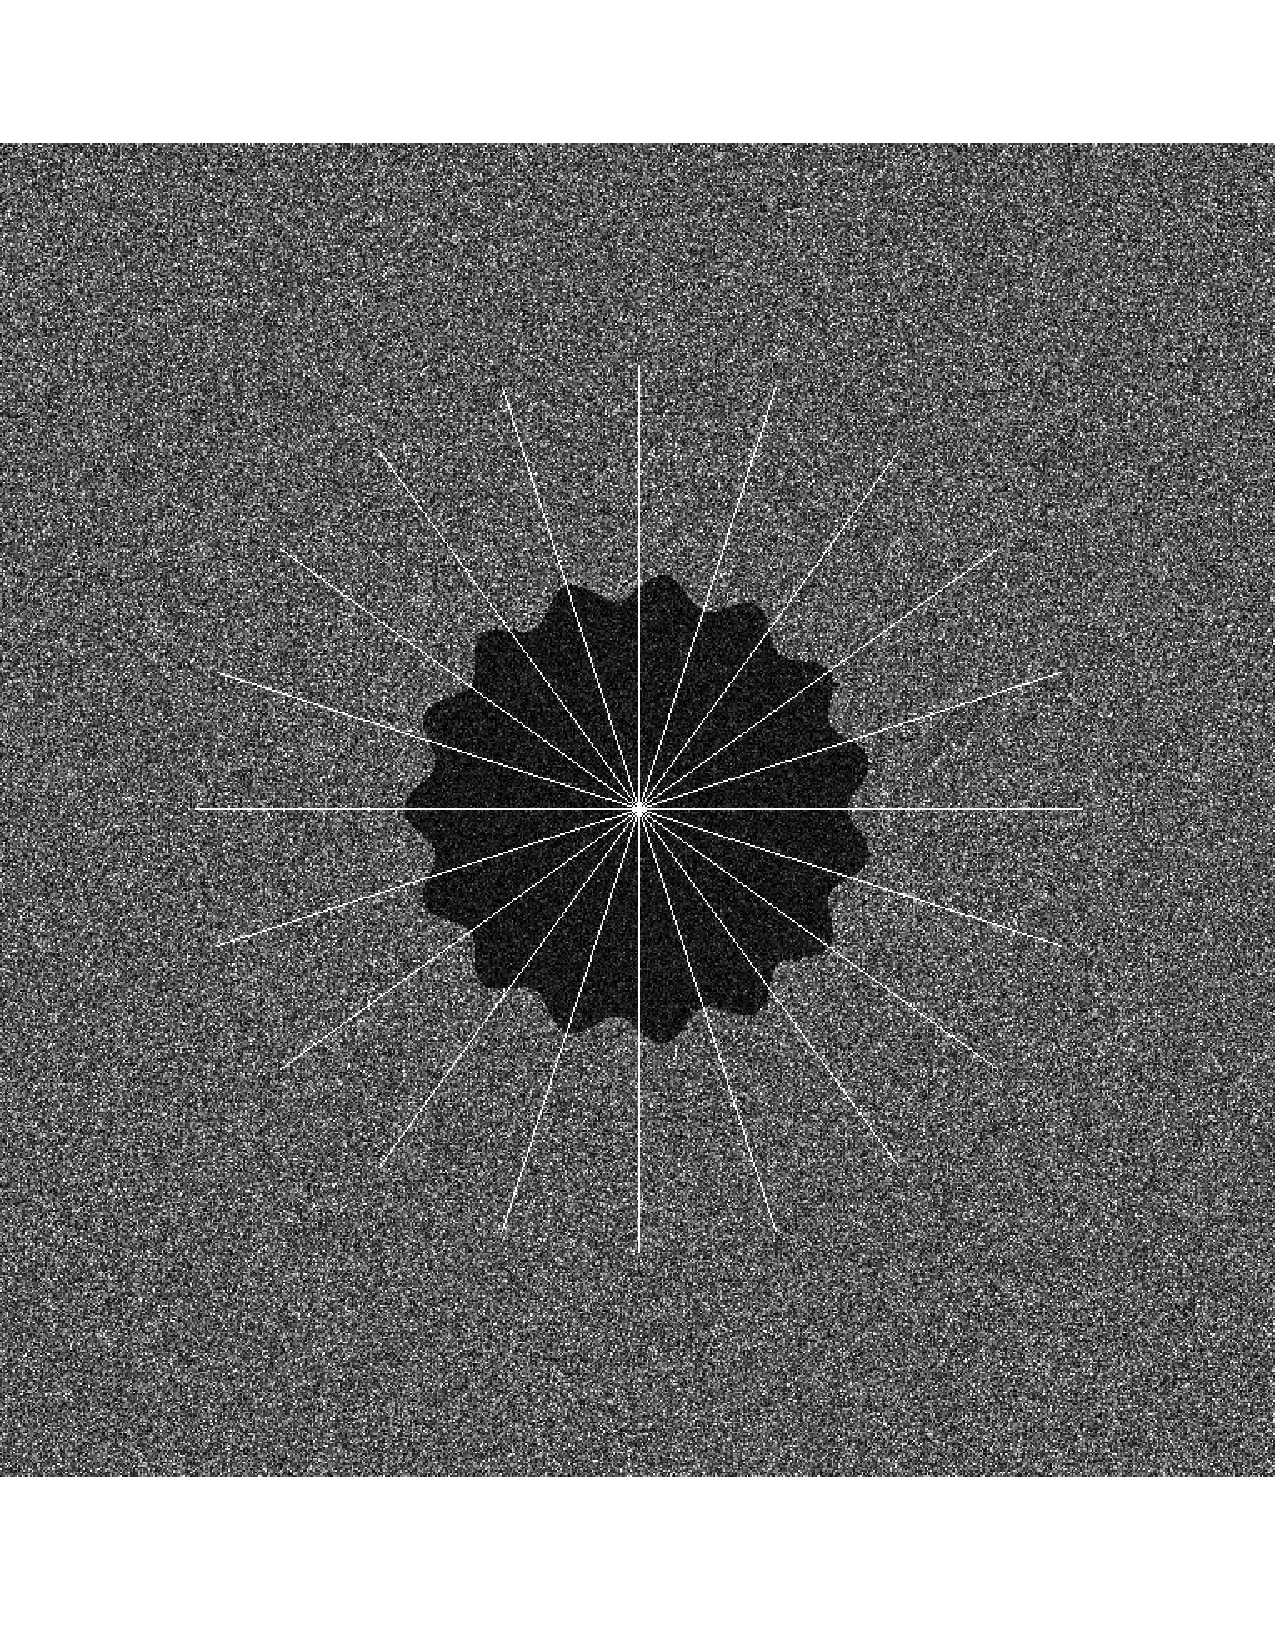
\includegraphics[width=\linewidth]{flor_15_133_8_hh.pdf}}
	\caption{Imagem flor simulada canal $I_{hh}$ com $\beta = 15$, $\delta = 133$ e $\nu = 8$ .}
\endminipage\hfill
\minipage{0.475\textwidth}
\fbox{ 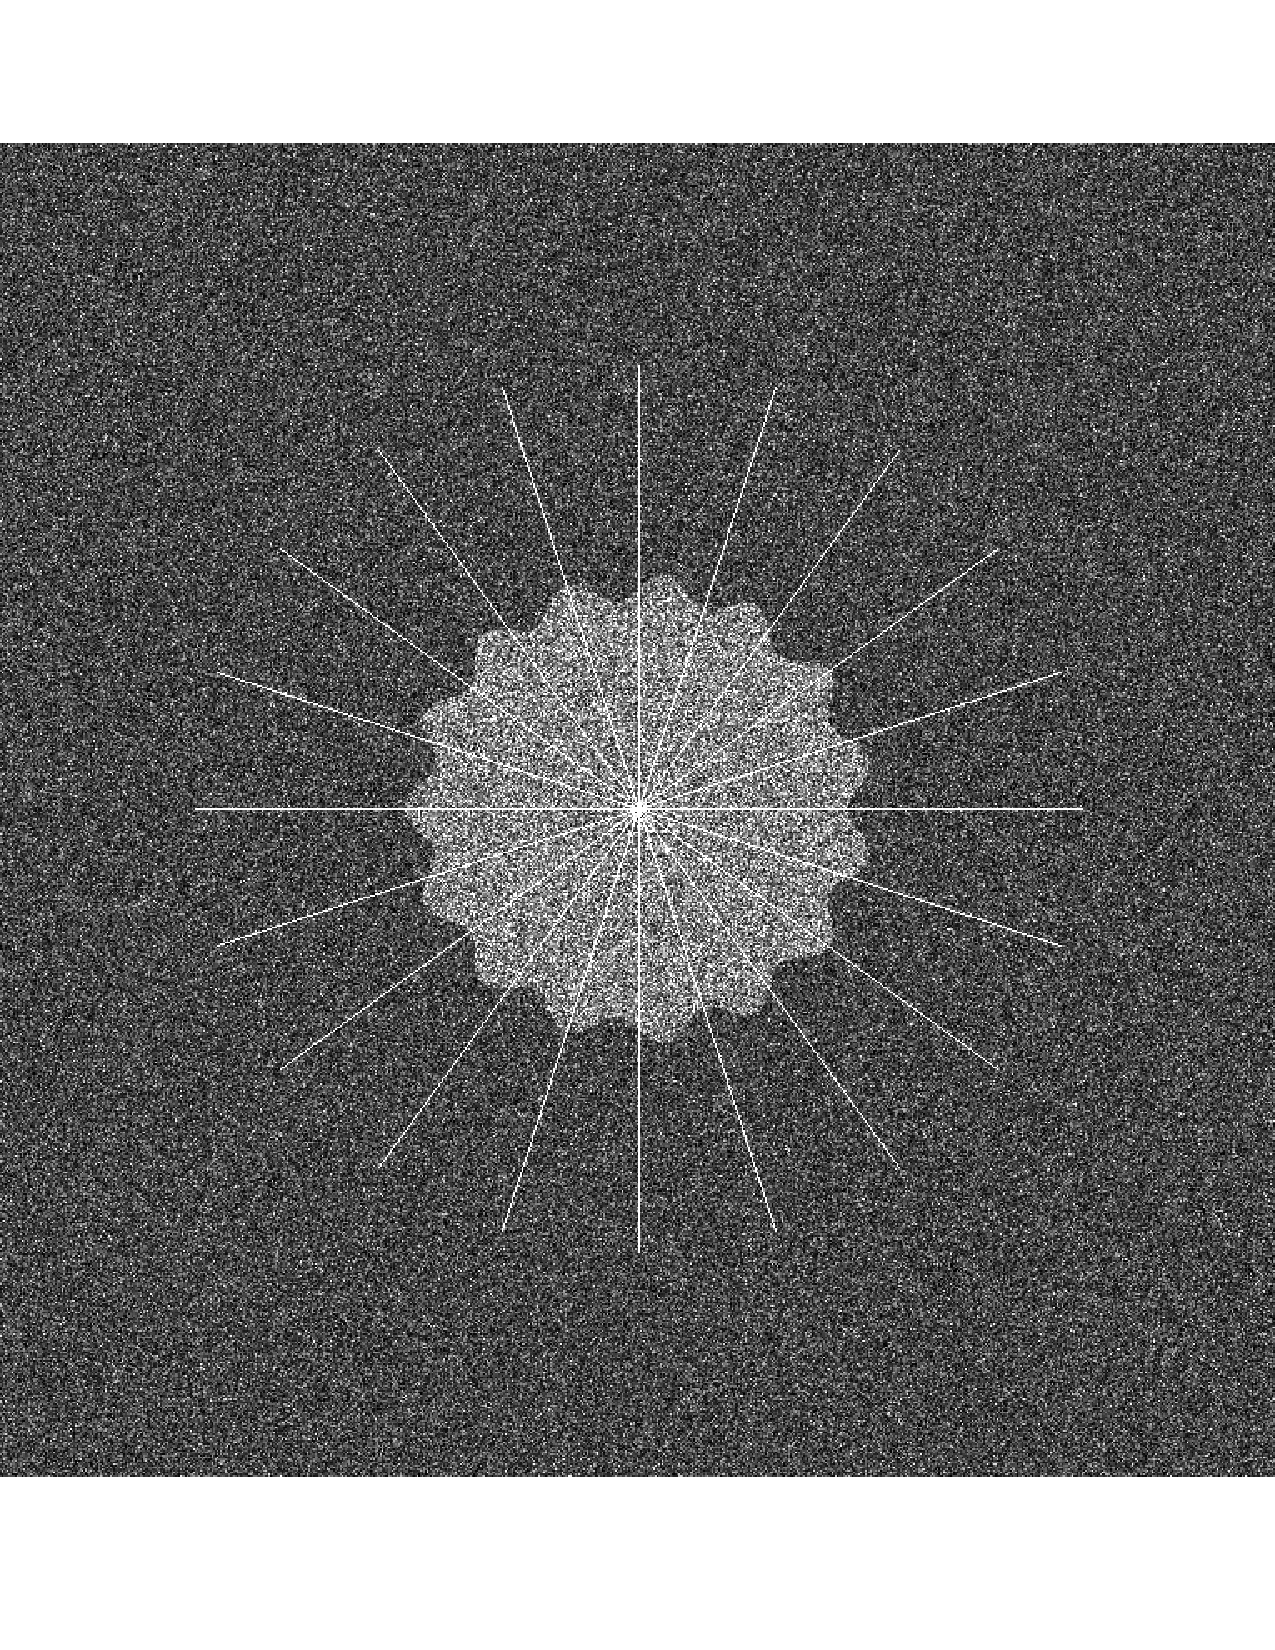
\includegraphics[width=\linewidth]{flor_15_133_8_hv.pdf}}
	\caption{Imagem flor simulada canal $I_{hv}$ com $\beta = 15$, $\delta = 133$ e $\nu = 8$ .}
\endminipage\hfill
\centering
\minipage{0.475\textwidth}
\fbox{ \includegraphics[width=\linewidth]{flor_15_133_8_vv.pdf}}
	\caption{Imagem flor simulada canal $I_{vv}$ com $\beta = 15$, $\delta = 133$ e $\nu = 8$ .}
\endminipage\hfill
\end{figure}
\begin{figure}[hbt]
	\fbox{\includegraphics[width=\linewidth]{flor_8_103_3_pauli.pdf}}
	\caption{Imagem flor simulada com $\beta = 8$, $\delta = 103$ e $\nu = 3$ .}
\label{cap_acf_fig15}
\end{figure}
\begin{figure}[hbt]
\minipage{0.475\textwidth}
	\fbox{\includegraphics[width=\linewidth]{flor_8_103_3_hh.pdf}}
	\caption{Imagem flor simulada canal $hh$ com $\beta = 8$, $\delta = 103$ e $\nu = 3$ .}
\label{cap_acf_fig15}
\endminipage\hfill
\minipage{0.475\textwidth}
	\fbox{\includegraphics[width=\linewidth]{flor_evid_8_103_3_hh.pdf}}
	\caption{Evidências de bordas canal $hh$ com $\beta = 8$, $\delta = 103$ e $\nu = 3$ .}
\label{cap_acf_fig16}
\endminipage\hfill
\end{figure}
\begin{figure}[hbt]
\minipage{0.475\textwidth}
	\fbox{\includegraphics[width=\linewidth]{flor_8_103_3_hv.pdf}}
	\caption{Imagem flor simulada canal $hv$ com $\beta = 8$, $\delta = 103$ e $\nu = 3$ .}
\label{cap_acf_fig15}
\endminipage\hfill
\minipage{0.475\textwidth}
	\fbox{\includegraphics[width=\linewidth]{flor_evid_8_103_3_hv.pdf}}
	\caption{Evidências de bordas canal $hv$ com $\beta = 8$, $\delta = 103$ e $\nu = 3$ .}
\label{cap_acf_fig16}
\endminipage\hfill
\end{figure}
\begin{figure}[hbt]
\minipage{0.475\textwidth}
	\fbox{\includegraphics[width=\linewidth]{flor_8_103_3_vv.pdf}}
	\caption{Imagem flor simulada canal $vv$ com $\beta = 8$, $\delta = 103$ e $\nu = 3$ .}
\label{cap_acf_fig15}
\endminipage\hfill
\minipage{0.475\textwidth}
	\fbox{\includegraphics[width=\linewidth]{flor_evid_8_103_3_vv.pdf}}
	\caption{Evidencias de bordas canal $vv$ com $\beta = 8$, $\delta = 103$ e $\nu = 3$ .}
\label{cap_acf_fig16}
\endminipage\hfill
\end{figure}
\begin{figure}[hbt]
	\fbox{\includegraphics[width=\linewidth]{flor_25_155_5_pauli.pdf}}
	\caption{Imagem flor simulada com $\beta = 25$, $\delta = 155$ e $\nu = 5$ .}
\label{cap_acf_fig15}
\end{figure}
\begin{figure}[hbt]
\minipage{0.475\textwidth}
	\fbox{\includegraphics[width=\linewidth]{flor_25_155_5_hh.pdf}}
	\caption{Imagem flor simulada canal $hh$ com $\beta = 25$, $\delta = 155$ e $\nu = 5$ .}
\label{cap_acf_fig15}
\endminipage\hfill
\minipage{0.475\textwidth}
	\fbox{\includegraphics[width=\linewidth]{flor_evid_25_155_5_hh.pdf}}
	\caption{Evidências de bordas canal $hh$ com $\beta = 25$, $\delta = 155$ e $\nu = 5$ .}
\label{cap_acf_fig16}
\endminipage\hfill
\end{figure}
\begin{figure}[hbt]
\minipage{0.475\textwidth}
	\fbox{\includegraphics[width=\linewidth]{flor_25_155_5_hv.pdf}}
	\caption{Imagem flor simulada canal $hv$ com $\beta = 25$, $\delta = 155$ e $\nu = 5$ .}
\label{cap_acf_fig15}
\endminipage\hfill
\minipage{0.475\textwidth}
	\fbox{\includegraphics[width=\linewidth]{flor_evid_25_155_5_hv.pdf}}
	\caption{Evidências de bordas canal $hv$ com $\beta = 25$, $\delta = 155$ e $\nu = 5$ .}
\label{cap_acf_fig16}
\endminipage\hfill
\end{figure}
\begin{figure}[hbt]
\minipage{0.475\textwidth}
	\fbox{\includegraphics[width=\linewidth]{flor_25_155_5_vv.pdf}}
	\caption{Imagem flor simulada canal $vv$ com $\beta = 25$, $\delta = 155$ e $\nu = 5$ .}
\label{cap_acf_fig15}
\endminipage\hfill
\minipage{0.475\textwidth}
	\fbox{\includegraphics[width=\linewidth]{flor_evid_25_155_5_vv.pdf}}
	\caption{Evidencias de bordas canal $vv$ com $\beta = 25$, $\delta = 155$ e $\nu = 5$ .}
\label{cap_acf_fig16}
\endminipage\hfill
\end{figure}
